% Options for packages loaded elsewhere
\PassOptionsToPackage{unicode}{hyperref}
\PassOptionsToPackage{hyphens}{url}
%
\documentclass[
]{article}
\usepackage{lmodern}
\usepackage{amssymb,amsmath}
\usepackage{ifxetex,ifluatex}
\ifnum 0\ifxetex 1\fi\ifluatex 1\fi=0 % if pdftex
  \usepackage[T1]{fontenc}
  \usepackage[utf8]{inputenc}
  \usepackage{textcomp} % provide euro and other symbols
\else % if luatex or xetex
  \usepackage{unicode-math}
  \defaultfontfeatures{Scale=MatchLowercase}
  \defaultfontfeatures[\rmfamily]{Ligatures=TeX,Scale=1}
\fi
% Use upquote if available, for straight quotes in verbatim environments
\IfFileExists{upquote.sty}{\usepackage{upquote}}{}
\IfFileExists{microtype.sty}{% use microtype if available
  \usepackage[]{microtype}
  \UseMicrotypeSet[protrusion]{basicmath} % disable protrusion for tt fonts
}{}
\makeatletter
\@ifundefined{KOMAClassName}{% if non-KOMA class
  \IfFileExists{parskip.sty}{%
    \usepackage{parskip}
  }{% else
    \setlength{\parindent}{0pt}
    \setlength{\parskip}{6pt plus 2pt minus 1pt}}
}{% if KOMA class
  \KOMAoptions{parskip=half}}
\makeatother
\usepackage{xcolor}
\IfFileExists{xurl.sty}{\usepackage{xurl}}{} % add URL line breaks if available
\IfFileExists{bookmark.sty}{\usepackage{bookmark}}{\usepackage{hyperref}}
\hypersetup{
  pdftitle={MatStat Problems},
  pdfauthor={Made by MatStatComeBack20-21},
  hidelinks,
  pdfcreator={LaTeX via pandoc}}
\urlstyle{same} % disable monospaced font for URLs
\usepackage[margin=1in]{geometry}
\usepackage{color}
\usepackage{fancyvrb}
\newcommand{\VerbBar}{|}
\newcommand{\VERB}{\Verb[commandchars=\\\{\}]}
\DefineVerbatimEnvironment{Highlighting}{Verbatim}{commandchars=\\\{\}}
% Add ',fontsize=\small' for more characters per line
\usepackage{framed}
\definecolor{shadecolor}{RGB}{248,248,248}
\newenvironment{Shaded}{\begin{snugshade}}{\end{snugshade}}
\newcommand{\AlertTok}[1]{\textcolor[rgb]{0.94,0.16,0.16}{#1}}
\newcommand{\AnnotationTok}[1]{\textcolor[rgb]{0.56,0.35,0.01}{\textbf{\textit{#1}}}}
\newcommand{\AttributeTok}[1]{\textcolor[rgb]{0.77,0.63,0.00}{#1}}
\newcommand{\BaseNTok}[1]{\textcolor[rgb]{0.00,0.00,0.81}{#1}}
\newcommand{\BuiltInTok}[1]{#1}
\newcommand{\CharTok}[1]{\textcolor[rgb]{0.31,0.60,0.02}{#1}}
\newcommand{\CommentTok}[1]{\textcolor[rgb]{0.56,0.35,0.01}{\textit{#1}}}
\newcommand{\CommentVarTok}[1]{\textcolor[rgb]{0.56,0.35,0.01}{\textbf{\textit{#1}}}}
\newcommand{\ConstantTok}[1]{\textcolor[rgb]{0.00,0.00,0.00}{#1}}
\newcommand{\ControlFlowTok}[1]{\textcolor[rgb]{0.13,0.29,0.53}{\textbf{#1}}}
\newcommand{\DataTypeTok}[1]{\textcolor[rgb]{0.13,0.29,0.53}{#1}}
\newcommand{\DecValTok}[1]{\textcolor[rgb]{0.00,0.00,0.81}{#1}}
\newcommand{\DocumentationTok}[1]{\textcolor[rgb]{0.56,0.35,0.01}{\textbf{\textit{#1}}}}
\newcommand{\ErrorTok}[1]{\textcolor[rgb]{0.64,0.00,0.00}{\textbf{#1}}}
\newcommand{\ExtensionTok}[1]{#1}
\newcommand{\FloatTok}[1]{\textcolor[rgb]{0.00,0.00,0.81}{#1}}
\newcommand{\FunctionTok}[1]{\textcolor[rgb]{0.00,0.00,0.00}{#1}}
\newcommand{\ImportTok}[1]{#1}
\newcommand{\InformationTok}[1]{\textcolor[rgb]{0.56,0.35,0.01}{\textbf{\textit{#1}}}}
\newcommand{\KeywordTok}[1]{\textcolor[rgb]{0.13,0.29,0.53}{\textbf{#1}}}
\newcommand{\NormalTok}[1]{#1}
\newcommand{\OperatorTok}[1]{\textcolor[rgb]{0.81,0.36,0.00}{\textbf{#1}}}
\newcommand{\OtherTok}[1]{\textcolor[rgb]{0.56,0.35,0.01}{#1}}
\newcommand{\PreprocessorTok}[1]{\textcolor[rgb]{0.56,0.35,0.01}{\textit{#1}}}
\newcommand{\RegionMarkerTok}[1]{#1}
\newcommand{\SpecialCharTok}[1]{\textcolor[rgb]{0.00,0.00,0.00}{#1}}
\newcommand{\SpecialStringTok}[1]{\textcolor[rgb]{0.31,0.60,0.02}{#1}}
\newcommand{\StringTok}[1]{\textcolor[rgb]{0.31,0.60,0.02}{#1}}
\newcommand{\VariableTok}[1]{\textcolor[rgb]{0.00,0.00,0.00}{#1}}
\newcommand{\VerbatimStringTok}[1]{\textcolor[rgb]{0.31,0.60,0.02}{#1}}
\newcommand{\WarningTok}[1]{\textcolor[rgb]{0.56,0.35,0.01}{\textbf{\textit{#1}}}}
\usepackage{graphicx,grffile}
\makeatletter
\def\maxwidth{\ifdim\Gin@nat@width>\linewidth\linewidth\else\Gin@nat@width\fi}
\def\maxheight{\ifdim\Gin@nat@height>\textheight\textheight\else\Gin@nat@height\fi}
\makeatother
% Scale images if necessary, so that they will not overflow the page
% margins by default, and it is still possible to overwrite the defaults
% using explicit options in \includegraphics[width, height, ...]{}
\setkeys{Gin}{width=\maxwidth,height=\maxheight,keepaspectratio}
% Set default figure placement to htbp
\makeatletter
\def\fps@figure{htbp}
\makeatother
\setlength{\emergencystretch}{3em} % prevent overfull lines
\providecommand{\tightlist}{%
  \setlength{\itemsep}{0pt}\setlength{\parskip}{0pt}}
\setcounter{secnumdepth}{-\maxdimen} % remove section numbering
\usepackage[utf8]{inputenc}
\usepackage{verbatim}
\usepackage[language]{babel}
\usepackage[encoding]{inputenc}
\usepackage{hyperref}
\usepackage{amsmath}
\usepackage{mathtools}
\usepackage{amssymb}
\usepackage{mathtools}
\usepackage{nicefrac}
\usepackage{fullpage}
\usepackage{stmaryrd}
\usepackage{aligned-overset}
\usepackage{pdfpages}

\title{MatStat Problems}
\author{Made by MatStatComeBack20-21}
\date{Last compiled on 09. juni, 2021}

\begin{document}
\maketitle

\begin{center}\rule{0.5\linewidth}{0.5pt}\end{center}

\newcommand{\C}{\mathbb{C}}

\newcommand{\R}{\mathbb{R}}

\newcommand{\Q}{\mathbb{Q}}

\newcommand{\Z}{\mathbb{Z}}

\newcommand{\N}{\mathbb{N}}

\newcommand{\E}{\mathbb{E}}

\newcommand{\F}{\mathbb{F}}

\newcommand{\B}{\mathbb{B}}

\newcommand{\K}{\mathbb{K}}

\newcommand{\RB}{\overline{\R}}

\newcommand{\ms}[1]{\mathscr{#1}}
\newcommand{\mc}[1]{\mathcal{#1}}
\newcommand{\BR}{\mathcal{B}\left(\R\right)}

\newcommand{\BRB}{\mathcal{B}\left(\RB\right))}

\newcommand{\mf}[1]{\mathfrak{#1}} 
\newcommand{\mcG}[2]{\mathcal{#1}^1(#2)} 
\newcommand{\mcGG}[4]{\mathcal{#1}_{#3}^{#2}(#4)}
\newcommand{\GMR}{\left(X,\ms{A},\mu\right)}

\newcommand{\PBS}{\lrp{\Omega,\F, P}}

\newcommand{\RMR}{\left(\R,\BR, \lambda\right)}

\newcommand{\MRBPBR}{\mc{M}_{\RB}^+\left(\BR\right)}

\newcommand{\MRPBR}{\mc{M}_{\R}^+\left(\BR\right)}

\newcommand{\Lp}[1]{L_{#1}\lrp{\lrs{0,1},m}} 
\newcommand{\mclxy}{\mc{L}\lrp{X,Y}}

\newcommand{\mckxy}{\mc{K}\lrp{X,Y}}

\newcommand{\mssr}{\ms{S}(\R)}

\newcommand{\ra}{\rightarrow}

\newcommand{\nra}{\nrightarrow}

\newcommand{\la}{\leftarrow}

\newcommand{\nla}{\nleftarrow}

\newcommand{\lra}{\leftrightarrow}

\newcommand{\nlra}{\nleftrightarrow}

\newcommand{\hra}{\hookrightarrow}

\newcommand{\Ra}{\Rightarrow}

\newcommand{\Lra}{\Leftrightarrow}

\newcommand{\Uda}{\Updownarrow}

\newcommand{\Da}{\Downarrow}

\newcommand{\rhpu}{\rightharpoonup}

\newcommand{\swel}{\overset{\swarrow}{=}}

\newcommand{\sweq}{\overset{\swarrow}{\equiv}}

\newcommand{\seel}{\overset{\searrow}{=}}

\newcommand{\seeq}{\overset{\searrow}{\equiv}}

\newcommand{\inse}{\overset{\cdot}{=}}

\newcommand{\PMX}{\mc{P}\left(X\right)}

\newcommand{\comp}{\mathsf{c}}

\newcommand{\sm}{\setminus}

\newcommand{\lrp}[1]{\left({#1}\right)}

\newcommand{\lrc}[1]{\left\{{#1}\right\}}

\newcommand{\lrs}[1]{\left[{#1}\right]}

\newcommand{\lrb}[1]{\left|{#1}\right|}

\newcommand{\inner}[2]{\left\langle #1, #2 \right\rangle}

\newcommand{\norm}[1]{\left\lVert#1\right\rVert}

\newcommand{\floor}[1]{\lfloor #1 \rfloor}

\newcommand{\ceil}[1]{\lceil #1 \rceil}

\newcommand{\FFou}[1]{\mc{F}(#1)}

\newcommand{\Fou}[1]{\widehat{#1}}

\newcommand{\blue}[1]{\textcolor{blue}{{#1}}}

\newcommand{\red}[1]{\textcolor{red}{{#1}}}

\newcommand{\green}[1]{\textcolor{green}{{#1}}}

\newcommand{\purple}[1]{\textcolor{purple}{{#1}}}

\newcommand{\cyan}[1]{\textcolor{cyan}{{#1}}}

\newcommand{\orange}[1]{\textcolor{orange}{{#1}}}

\newcommand{\boldhat}[1]{\mathbf{\hat{\text{$#1$}}}}
\newcommand{\boldbar}[1]{\mathbf{\bar{\text{$#1$}}}}
\newcommand{\boldtilde}[1]{\mathbf{\tilde{\text{$#1$}}}}
\newcommand{\boldcheck}[1]{\mathbf{\check{\text{$#1$}}}}

\newcommand{\indep}{\perp \!\!\! \perp}

\newcommand{\colvec}[1]{\begin{pmatrix}{#1}\end{pmatrix}}

\newcommand{\nd}[2]{\mc{N}\lrp{{#1},{#2}}}

\newcommand{\dnd}[2]{\sim\mc{N}\lrp{{#1},{#2}}}

\hypertarget{hs-problems}{%
\section{HS Problems}\label{hs-problems}}

\hypertarget{hs-1-in-danish}{%
\subsection{HS 1 (In danish)}\label{hs-1-in-danish}}

\hypertarget{section}{%
\paragraph{\texorpdfstring{\textbf{1.}}{1.}}\label{section}}

Vi kører de efterspurgte kommandoer

\begin{Shaded}
\begin{Highlighting}[]
\CommentTok{## library(MASS)}
\CommentTok{## cats}
\KeywordTok{head}\NormalTok{(cats)}
\end{Highlighting}
\end{Shaded}

\begin{verbatim}
##   Sex Bwt Hwt
## 1   F 2.0 7.0
## 2   F 2.0 7.4
## 3   F 2.0 9.5
## 4   F 2.1 7.2
## 5   F 2.1 7.3
## 6   F 2.1 7.6
\end{verbatim}

\begin{Shaded}
\begin{Highlighting}[]
\KeywordTok{dim}\NormalTok{(cats)}
\end{Highlighting}
\end{Shaded}

\begin{verbatim}
## [1] 144   3
\end{verbatim}

\begin{Shaded}
\begin{Highlighting}[]
\KeywordTok{summary}\NormalTok{(cats)}
\end{Highlighting}
\end{Shaded}

\begin{verbatim}
##  Sex         Bwt             Hwt       
##  F:47   Min.   :2.000   Min.   : 6.30  
##  M:97   1st Qu.:2.300   1st Qu.: 8.95  
##         Median :2.700   Median :10.10  
##         Mean   :2.724   Mean   :10.63  
##         3rd Qu.:3.025   3rd Qu.:12.12  
##         Max.   :3.900   Max.   :20.50
\end{verbatim}

Vi kan samtidigt også importere cats et datasæt i R i stedet for som en
del af \texttt{cats} pakken, idet vi erklærer;

\begin{Shaded}
\begin{Highlighting}[]
\NormalTok{cats <-}\StringTok{ }\NormalTok{cats}
\end{Highlighting}
\end{Shaded}

\hypertarget{section-1}{%
\paragraph{\texorpdfstring{\textbf{2.}}{2.}}\label{section-1}}

Bemærk at vi i \texttt{cats} datasættet har med forskellige enheder at
gøre. Specifikt er det således at \texttt{Bwt} er i kilogram, mens
\texttt{Hwt} er i gram. For at udregne forholdet mellem \texttt{Hwt} og
\texttt{Bwt}, for så da at kunne omsætte til procent, må vi altså have
dem på samme enhed. I dette tilfælde vil vi regne i kg, så vi ganger
\texttt{Hwt} med \(1=\frac{1kg}{1000g},\) for da at tage forholdet
\texttt{Hwt/Bwt} og tilsidst gange med \(100\) for at få resultatet i
procent. Den resulterende transformation, efterfulgt af et fornyet kig
på \texttt{head(cats)}

\begin{Shaded}
\begin{Highlighting}[]
\NormalTok{cats <-}\StringTok{ }\KeywordTok{transform}\NormalTok{(cats, }\DataTypeTok{pct =}\NormalTok{ (cats}\OperatorTok{$}\NormalTok{Hwt}\OperatorTok{/}\DecValTok{1000}\NormalTok{)}\OperatorTok{*}\NormalTok{(}\DecValTok{1}\OperatorTok{/}\NormalTok{cats}\OperatorTok{$}\NormalTok{Bwt)}\OperatorTok{*}\DecValTok{100}\NormalTok{)}
\KeywordTok{head}\NormalTok{(cats)}
\end{Highlighting}
\end{Shaded}

\begin{verbatim}
##   Sex Bwt Hwt       pct
## 1   F 2.0 7.0 0.3500000
## 2   F 2.0 7.4 0.3700000
## 3   F 2.0 9.5 0.4750000
## 4   F 2.1 7.2 0.3428571
## 5   F 2.1 7.3 0.3476190
## 6   F 2.1 7.6 0.3619048
\end{verbatim}

Således at vi eksempelvis i række to har at hjertevægten af kat nummer
to udgør smålige \(0,37\%\) af kropsvægten af katten - overraskende
lidt.

\hypertarget{section-2}{%
\paragraph{\texorpdfstring{\textbf{3.}}{3.}}\label{section-2}}

As requested we may subset \texttt{cats} with the \texttt{subset}
function, remembering that any gentleman always defines
\texttt{femaleData} first;

\begin{Shaded}
\begin{Highlighting}[]
\NormalTok{femaleData <-}\StringTok{ }\KeywordTok{subset}\NormalTok{(cats, cats}\OperatorTok{$}\NormalTok{Sex }\OperatorTok{==}\StringTok{ "F"}\NormalTok{)}
\NormalTok{maleData <-}\StringTok{ }\KeywordTok{subset}\NormalTok{(cats, cats}\OperatorTok{$}\NormalTok{Sex }\OperatorTok{==}\StringTok{ "M"}\NormalTok{)}
\KeywordTok{head}\NormalTok{(femaleData)}
\end{Highlighting}
\end{Shaded}

\begin{verbatim}
##   Sex Bwt Hwt       pct
## 1   F 2.0 7.0 0.3500000
## 2   F 2.0 7.4 0.3700000
## 3   F 2.0 9.5 0.4750000
## 4   F 2.1 7.2 0.3428571
## 5   F 2.1 7.3 0.3476190
## 6   F 2.1 7.6 0.3619048
\end{verbatim}

\begin{Shaded}
\begin{Highlighting}[]
\KeywordTok{head}\NormalTok{(maleData)}
\end{Highlighting}
\end{Shaded}

\begin{verbatim}
##    Sex Bwt  Hwt       pct
## 48   M 2.0  6.5 0.3250000
## 49   M 2.0  6.5 0.3250000
## 50   M 2.1 10.1 0.4809524
## 51   M 2.2  7.2 0.3272727
## 52   M 2.2  7.6 0.3454545
## 53   M 2.2  7.9 0.3590909
\end{verbatim}

\hypertarget{hs-2}{%
\subsection{HS 2}\label{hs-2}}

\hypertarget{section-3}{%
\paragraph{\texorpdfstring{\textbf{1.}}{1.}}\label{section-3}}

We will be testing a linear regression model on the data prepared in
HS1. Starting off with a \texttt{(Bwt,Hwt)} scatterplot, note once again
that \texttt{Hwt} is in units of grams, with \texttt{Bwt} being in
kilograms.

\begin{Shaded}
\begin{Highlighting}[]
\KeywordTok{plot}\NormalTok{(cats}\OperatorTok{$}\NormalTok{Bwt,cats}\OperatorTok{$}\NormalTok{Hwt, }\DataTypeTok{main =} \StringTok{"(Bwt, Hwt) scatterplot"}\NormalTok{, }\DataTypeTok{xlab =} \StringTok{"Cat bodyweight in kg"}\NormalTok{, }\DataTypeTok{ylab =} \StringTok{"Cat heartweight in g"}\NormalTok{)}
\end{Highlighting}
\end{Shaded}

\begin{center}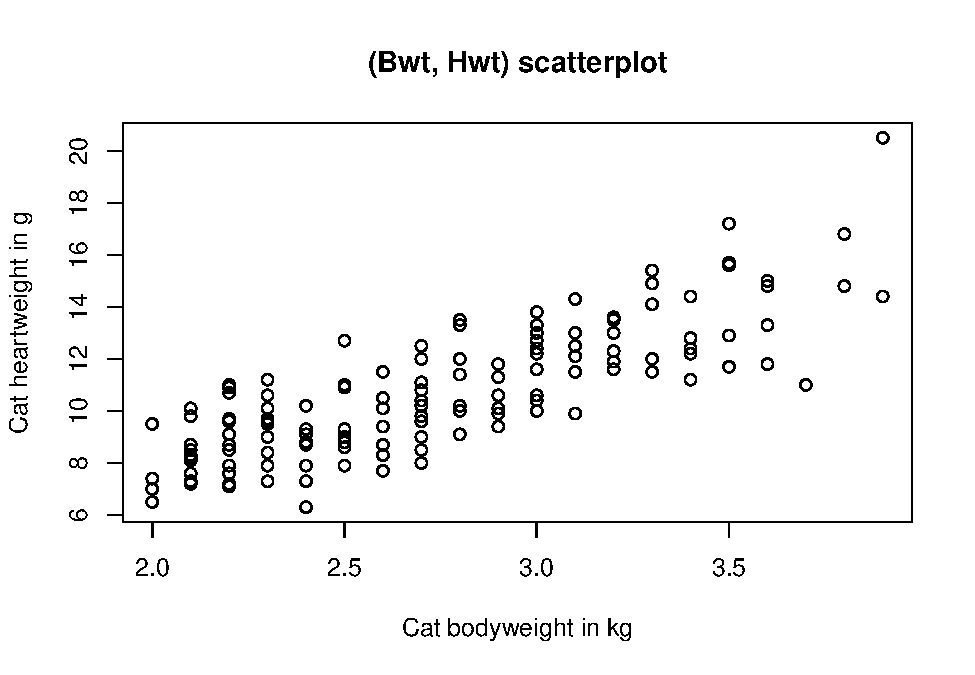
\includegraphics{matstatproblems20-21_files/figure-latex/unnamed-chunk-5-1} \end{center}

The statistical model behind the linear regression may be recited from
Definition 6.1 of ``Introduktion til Statistik''.

\emph{We assume
\(Y_1,\ldots,Y_n \overset{\text{iid.}}{\sim}\mathcal{N}(\alpha+\beta x_i,\sigma^2),\,\)with
\(\alpha,\beta\in\mathbb{R},\,\sigma^2>0\) being unknown parameters.}

Finally we will for \texttt{maleData} be using the \texttt{lm}-function
in 
\includegraphics[width=\textwidth,height=0.16667in]{R_logo.png} to
fit the linear regression model to the \texttt{maleData}, assuming
heartweight to be a linear function of bodyweight such that we might
write \texttt{Hwt} \(= \alpha + \beta\,\cdot\)\texttt{Bwt}.

\begin{Shaded}
\begin{Highlighting}[]
\NormalTok{linreg <-}\StringTok{ }\KeywordTok{lm}\NormalTok{(Hwt }\OperatorTok{~}\StringTok{ }\NormalTok{Bwt, }\DataTypeTok{data =}\NormalTok{ maleData)}
\end{Highlighting}
\end{Shaded}

\hypertarget{section-4}{%
\paragraph{\texorpdfstring{\textbf{2.}}{2.}}\label{section-4}}

Further following the procedures of Chapter 6 (in particular page 133)
in ``Introduktion til Statistik'' we might complete a visual model
validation of our linear regression model by getting

\includegraphics[width=\textwidth,height=0.16667in]{R_logo.png} to
calculate the estimated values of the model, and the standardized
residuals of the data also. Respectively, this will be done with the
assignment

\begin{Shaded}
\begin{Highlighting}[]
\NormalTok{fit <-}\StringTok{ }\KeywordTok{fitted}\NormalTok{(linreg)}
\NormalTok{rst <-}\StringTok{ }\KeywordTok{rstandard}\NormalTok{(linreg)}
\end{Highlighting}
\end{Shaded}

such that we might plot the fitted values against the standardized
residuals, adding a horizontal line through zero also

\begin{Shaded}
\begin{Highlighting}[]
\KeywordTok{plot}\NormalTok{(fit, rst, }\DataTypeTok{main =} \StringTok{"(Estimate, Std. Res.)-plot for linreg model on maleData"}\NormalTok{, }\DataTypeTok{xlab =} \StringTok{"Estimated (fitted) Heartweight (g)"}\NormalTok{, }\DataTypeTok{ylab =}\StringTok{"Standardized residuals"}\NormalTok{, }\DataTypeTok{ylim =} \KeywordTok{c}\NormalTok{(}\OperatorTok{-}\KeywordTok{max}\NormalTok{(}\FloatTok{3.2}\NormalTok{,}\KeywordTok{max}\NormalTok{(}\KeywordTok{abs}\NormalTok{(rst))), }\KeywordTok{max}\NormalTok{(}\FloatTok{3.2}\NormalTok{,}\KeywordTok{max}\NormalTok{(}\KeywordTok{abs}\NormalTok{(rst)))) ) }\CommentTok{#Largest symmetric interval (around 0) of (-3.2,3.2) or (-largest absolute rst, largest absolute rst)}
\KeywordTok{abline}\NormalTok{(}\DecValTok{0}\NormalTok{,}\DecValTok{0}\NormalTok{)}
\end{Highlighting}
\end{Shaded}

\begin{center}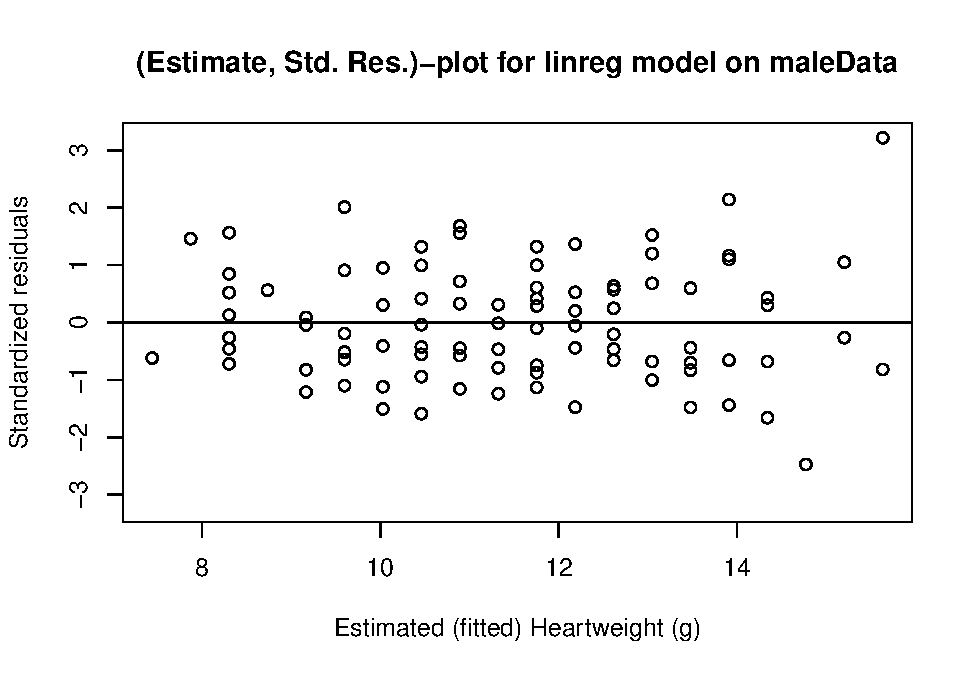
\includegraphics{matstatproblems20-21_files/figure-latex/unnamed-chunk-8-1} \end{center}

Looking at the above plot, we note that if the assumption that the
variance of the heartweight data is independent of the mean is true, we
would expect that the dispersion of points at region of fitted
heartweight values would be akin to the dispersion in any other
region.If the linearity assumption of our model were to be true, we
would expect the points to be relatively equally dispersed as
\(\mathcal{N}(0,1)\) on both sides of \(0\) across the fitted values. -
ie. that the standardized residuals are themselves rather
\(\mathcal{N}(0,1)\) distributed.

The plot looks rather respectable on both these fronts, as 1. The
residual values fall within the interval \(\left({-2,2}\right),\) as
would be expected of a standard normal distribution. 2. No wierd
``trumpet'', ``quadratic'' or other wierd distortions to the std.
residuals values are present, they seem to keep rather constantly
dispersed around zero within any fitted heartweight region.

Note that the values of

\begin{Shaded}
\begin{Highlighting}[]
\KeywordTok{mean}\NormalTok{(rst)}
\end{Highlighting}
\end{Shaded}

\begin{verbatim}
## [1] 0.0004535485
\end{verbatim}

\begin{Shaded}
\begin{Highlighting}[]
\KeywordTok{var}\NormalTok{(rst)}
\end{Highlighting}
\end{Shaded}

\begin{verbatim}
## [1] 1.015539
\end{verbatim}

fit in line.

Finally the assumption that the heartweight data is normally distributed
may be visually assessed through the use of a QQ-plot of the
standardized residuals. If the normallity assumption of the model were
to be true we would expect the standardized residuals to be
\(\mathcal{N}(0,1)\) distributed, which would reveal itself if the
points if the theoretical \(\mathcal{N}(0,1)\) quantiles were to match
the empirical quantiles of the standardized residuals, such that the
points of the QQ-plot were to hug the line intersecting the mean \(0\)
and with slope equal to the standard deviation of an
\(\mathcal{N}(0,1)\) distributed value, ie. with slope \(\sqrt{1}=1\).
The plot and the corresponding line intersecting \(0\) and having slope
\(1\) can be made with the commands below

\begin{Shaded}
\begin{Highlighting}[]
\KeywordTok{qqnorm}\NormalTok{(rst)}
\KeywordTok{abline}\NormalTok{(}\DecValTok{0}\NormalTok{,}\DecValTok{1}\NormalTok{)}
\end{Highlighting}
\end{Shaded}

\begin{center}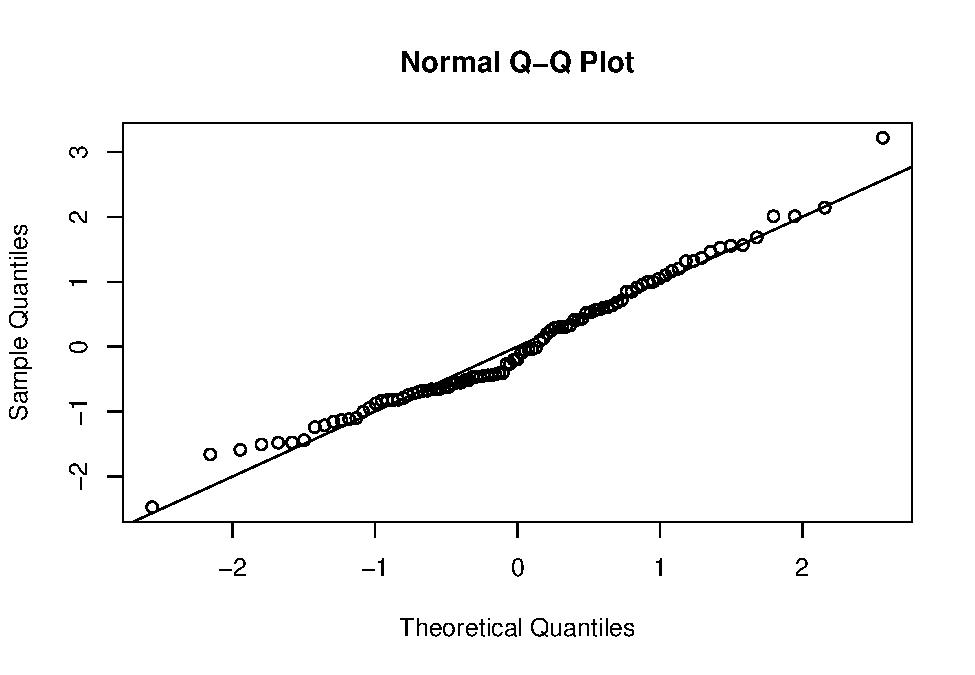
\includegraphics{matstatproblems20-21_files/figure-latex/unnamed-chunk-10-1} \end{center}

revealing that no sufficiently large abnormalities seem to be present
that would disprove our theory that the standardized residuals are
\(\mathcal{N}(0,1)\) distributed, and thus, that the data follows a
normal distribution also. Do however observe, that making a QQ-plot of
the data itself won't lead to much fruition, as the means are assumed to
vary according to the bodyweight (unless ofcourse we have \(\beta=0\)).

All in all, we say that it seems fairly reasonable to assume that the
data is distributed according to the above written model.

\hypertarget{section-5}{%
\paragraph{\texorpdfstring{\textbf{3.}}{3.}}\label{section-5}}

A valueable way to get insight into the linear regression model made by

\includegraphics[width=\textwidth,height=0.16667in]{R_logo.png} is to
deploy the \texttt{summary} function.

\begin{Shaded}
\begin{Highlighting}[]
\KeywordTok{summary}\NormalTok{(linreg)}
\end{Highlighting}
\end{Shaded}

\begin{verbatim}
## 
## Call:
## lm(formula = Hwt ~ Bwt, data = maleData)
## 
## Residuals:
##     Min      1Q  Median      3Q     Max 
## -3.7728 -1.0478 -0.2976  0.9835  4.8646 
## 
## Coefficients:
##             Estimate Std. Error t value Pr(>|t|)    
## (Intercept)  -1.1841     0.9983  -1.186    0.239    
## Bwt           4.3127     0.3399  12.688   <2e-16 ***
## ---
## Signif. codes:  0 '***' 0.001 '**' 0.01 '*' 0.05 '.' 0.1 ' ' 1
## 
## Residual standard error: 1.557 on 95 degrees of freedom
## Multiple R-squared:  0.6289, Adjusted R-squared:  0.625 
## F-statistic:   161 on 1 and 95 DF,  p-value: < 2.2e-16
\end{verbatim}

which reveals a rather lot of details around the fitted linear model.
Information of how to interpret the output of \texttt{summary} may be
found through the \texttt{?lm}-command.

Another valuable trick is that it is possible to draw out the
slope(\(\beta\)) and intersect (\(\alpha\)) values for the linear
regression of the data, and use these to define local variables
\texttt{beta} and \texttt{alpha} through c(1,2,3,4)

\begin{Shaded}
\begin{Highlighting}[]
\NormalTok{alpha <-}\StringTok{ }\NormalTok{linreg}\OperatorTok{$}\NormalTok{coefficients[[}\DecValTok{1}\NormalTok{]]}
\end{Highlighting}
\end{Shaded}

\begin{verbatim}
## [1] -1.184088
\end{verbatim}

\begin{Shaded}
\begin{Highlighting}[]
\NormalTok{beta <-}\StringTok{ }\NormalTok{linreg}\OperatorTok{$}\NormalTok{coefficients[[}\DecValTok{2}\NormalTok{]]}
\end{Highlighting}
\end{Shaded}

\begin{verbatim}
## [1] 4.312679
\end{verbatim}

Noting the use of \texttt{{[}{[}{]}{]}} to extract the numerical value
instead of a named value as results from using

\begin{Shaded}
\begin{Highlighting}[]
\NormalTok{linreg}\OperatorTok{$}\NormalTok{coefficients[}\DecValTok{1}\NormalTok{]}
\end{Highlighting}
\end{Shaded}

\begin{verbatim}
## (Intercept) 
##   -1.184088
\end{verbatim}

\begin{Shaded}
\begin{Highlighting}[]
\NormalTok{linreg}\OperatorTok{$}\NormalTok{coefficients[}\DecValTok{2}\NormalTok{]}
\end{Highlighting}
\end{Shaded}

\begin{verbatim}
##      Bwt 
## 4.312679
\end{verbatim}

Alternatively the format,

\begin{Shaded}
\begin{Highlighting}[]
\KeywordTok{as.numeric}\NormalTok{(linreg}\OperatorTok{$}\NormalTok{coefficients[}\DecValTok{1}\NormalTok{])}
\end{Highlighting}
\end{Shaded}

\begin{verbatim}
## [1] -1.184088
\end{verbatim}

\begin{Shaded}
\begin{Highlighting}[]
\KeywordTok{as.numeric}\NormalTok{(linreg}\OperatorTok{$}\NormalTok{coefficients[}\DecValTok{2}\NormalTok{])}
\end{Highlighting}
\end{Shaded}

\begin{verbatim}
## [1] 4.312679
\end{verbatim}

evidently works as well.

We have thus established the model that \texttt{maleData\$Hwt\ =}
-1.1840879 \texttt{+} 4.3126787 \texttt{maleData\$Bwt}. As the rate
change of an affine function is constant we may just note that an
increase in bodyweight of \(0.5kg,\) will by the model provide an
\texttt{0.5\ beta\ =} 2.1563394gram increase in heartweight.

Note that the model is rather imperfect, as it for example for
\texttt{maledata\$Bwt} \(\searrow 0 kg\) estimates
\texttt{maleData\$Hwt} \(\searrow -1.1840879 g\). And while the above
problem to the model is of course in itself preposterous, we may note
that if we wanted to force

\includegraphics[width=\textwidth,height=0.16667in]{R_logo.png} to fit
the best linear model to the data assuming intersection at zero, we
might've done this through the use of
\texttt{linreg\ \textless{}-\ lm(Hwt\ \textasciitilde{}\ Bwt\ -\ 1,\ data\ =\ maleData)}
ie. with the inclusion of ``-1'' being the symbolic manipulation
required to tell

\includegraphics[width=\textwidth,height=0.16667in]{R_logo.png} to model
based on the assumption of intersection in \(0.\)

\hypertarget{section-6}{%
\paragraph{\texorpdfstring{\textbf{4.}}{4.}}\label{section-6}}

Let us just remind ourselves of the standard frequentistic
interpretation ascribed to confidence intervals of level \(1-\alpha^*\)
for the parameter \(\beta\):

Imagine the experiment being conducted multiple times in the same way,
but independent of the original and each other - in our case a new batch
of cats being weighed, their sex noted, and their heartweight noted
also. Using the dataset corresponding to each repetition of experiment
we calculate the \(1-\alpha^*\) confidence intervals for \(\beta\) (as
will be done below). We would then expect the true value of \(\beta\) to
be present in approximately ratio \(1-\alpha^*\) of all the intervals
calculated.

From Theorem 6.9 in ``Introduktion to Statistik'' we have that an
\(1-\alpha^*\) confidence-interval for \(\beta\) can be found as the
interval bounded by \[\hat{\beta}\pm t_{n-2,1-alpha^*/2}SE(\hat\beta)\]
Note that we may find the standard error for \(\beta,\,SE(\hat\beta)\)
in \texttt{summary(linreg)} as ``std error for Bwt'', which is
\texttt{0.3399} in our instance. Extraction of this value might occur
via

\begin{Shaded}
\begin{Highlighting}[]
\NormalTok{seb <-}\StringTok{ }\KeywordTok{sqrt}\NormalTok{(}\KeywordTok{diag}\NormalTok{(}\KeywordTok{vcov}\NormalTok{(linreg)))[[}\DecValTok{2}\NormalTok{]]}
\end{Highlighting}
\end{Shaded}

\begin{verbatim}
## [1] 0.3398942
\end{verbatim}

Having taken a look at \texttt{?qt} as well as an extra look at Theorem
6.9, we may in order to get an \(95\%\) confidence interval do

\begin{Shaded}
\begin{Highlighting}[]
\NormalTok{n <-}\StringTok{ }\KeywordTok{nrow}\NormalTok{(maleData)}
\end{Highlighting}
\end{Shaded}

\begin{verbatim}
## [1] 97
\end{verbatim}

\begin{Shaded}
\begin{Highlighting}[]
\NormalTok{lKI <-}\StringTok{ }\NormalTok{beta }\OperatorTok{-}\StringTok{ }\KeywordTok{qt}\NormalTok{(}\FloatTok{0.975}\NormalTok{, n}\DecValTok{-2}\NormalTok{)}\OperatorTok{*}\NormalTok{seb}
\NormalTok{uKI <-}\StringTok{ }\NormalTok{beta }\OperatorTok{+}\StringTok{ }\KeywordTok{qt}\NormalTok{(}\FloatTok{0.975}\NormalTok{, n}\DecValTok{-2}\NormalTok{)}\OperatorTok{*}\NormalTok{seb}
\NormalTok{KI <-}\StringTok{ }\KeywordTok{c}\NormalTok{(lKI, uKI)}
\end{Highlighting}
\end{Shaded}

\begin{verbatim}
## [1] 3.637904 4.987454
\end{verbatim}

ie we get the \(95\%\) confidence-interval
\texttt{(3.6379035,4.987454)}.

\hypertarget{section-7}{%
\paragraph{\texorpdfstring{\textbf{5.}}{5.}}\label{section-7}}

Having browsed \texttt{?confint} we may refind the results of the
previous subproblem with \texttt{confint(linreg)} as follows;

\begin{Shaded}
\begin{Highlighting}[]
\KeywordTok{confint}\NormalTok{(linreg)}
\end{Highlighting}
\end{Shaded}

\begin{verbatim}
##                 2.5 %    97.5 %
## (Intercept) -3.165939 0.7977636
## Bwt          3.637904 4.9874540
\end{verbatim}

\begin{Shaded}
\begin{Highlighting}[]
\CommentTok{#We try to extract the interval;}
\KeywordTok{confint}\NormalTok{(linreg)[}\DecValTok{2}\NormalTok{,]}
\end{Highlighting}
\end{Shaded}

\begin{verbatim}
##    2.5 %   97.5 % 
## 3.637904 4.987454
\end{verbatim}

\begin{Shaded}
\begin{Highlighting}[]
\KeywordTok{as.numeric}\NormalTok{(}\KeywordTok{confint}\NormalTok{(linreg)[}\DecValTok{2}\NormalTok{,]) }\CommentTok{#KI}
\end{Highlighting}
\end{Shaded}

\begin{verbatim}
## [1] 3.637904 4.987454
\end{verbatim}

\begin{Shaded}
\begin{Highlighting}[]
\KeywordTok{confint}\NormalTok{(linreg)[}\DecValTok{2}\NormalTok{,}\DecValTok{1}\NormalTok{] }\CommentTok{#lKI}
\end{Highlighting}
\end{Shaded}

\begin{verbatim}
## [1] 3.637904
\end{verbatim}

\begin{Shaded}
\begin{Highlighting}[]
\KeywordTok{confint}\NormalTok{(linreg)[}\DecValTok{2}\NormalTok{,}\DecValTok{2}\NormalTok{] }\CommentTok{#uKI}
\end{Highlighting}
\end{Shaded}

\begin{verbatim}
## [1] 4.987454
\end{verbatim}

\hypertarget{section-8}{%
\paragraph{\texorpdfstring{\textbf{6.}}{6.}}\label{section-8}}

For \(x_i\) being the bodyweight data and \(Y_i\) being the stochastic
variable representing the heartweight both of the \(i\)'th male cat, we
will by assumption have \(E(Y_i)=\alpha + \beta x_i.\) Finding a
designmatrix \(A\) such that we way write
\(\xi:=\left({E(Y_1), E(Y_2), \ldots, E(Y_{97})}\right)^T\) as \[
\xi=A\begin{pmatrix}
\alpha\\
\beta
\end{pmatrix}.
\] Consequently, as
\(\xi\in M_{97,1}(\mathbb{R}),\,\left({\alpha, \beta}\right)^T\in M_{2,1}(\mathbb{R}),\)
we will by matrix multiplication need to have
\(A\in M_{97,2}(\mathbb{R}),\) and in particular for \begin{align*}
A\begin{pmatrix}
\alpha\\
\beta
\end{pmatrix}
\overset{\swarrow}{\equiv}
\begin{pmatrix}
a_{1,1} & a_{1,2} \\
a_{2,1} & a_{2,2} \\
\vdots & \vdots \\
a_{97,1} & a_{97,2}
\end{pmatrix}\begin{pmatrix}
\alpha\\
\beta
\end{pmatrix}&\overset{\swarrow}{=}
\begin{pmatrix}
a_{1,1}\alpha + a_{1,2}\beta \\
a_{2,1}\alpha + a_{2,2}\beta \\
\vdots \\
a_{97,1}\alpha+a_{97,2}\beta 
\end{pmatrix}\overset{\searrow}{=}\begin{pmatrix}
\alpha + \beta x_1 \\
\alpha + \beta x_2 \\
\vdots \\
\alpha + \beta x_{97} \\
\end{pmatrix}\overset{\searrow}{\equiv}\xi\\
&\Leftrightarrow\\
a_{i,1}\equiv 1&,\,\,a_{i,2}=x_i\\
&\Leftrightarrow\\
A&=\begin{pmatrix}
1 & x_1 \\
1 & x_2 \\
\vdots & \vdots \\
1 & x_{97}
\end{pmatrix}
\end{align*}

\hypertarget{hs-3}{%
\subsection{HS 3}\label{hs-3}}

\hypertarget{section-9}{%
\paragraph{\texorpdfstring{\textbf{1.}}{1.}}\label{section-9}}

We may recite the (normal) statistical model of two independent samples
as given in D. 5.1 of ``Introduktion til Statistik'';

\emph{Let \(X_1,\ldots,X_{n_1}\) and \(Y_1,\ldots,Y_{n_2}\) be
independent normally distributed random variables with
\(X_i\sim\mathcal{N}(\mu_1,\sigma^2)\) and
\(Y_j\sim\mathcal{N}(\mu_2,\sigma^2),\) with
\(\mu_1,\mu_2\in\mathbb{R}\) and \(\sigma^2>0\) being unknown
parameters}

\hypertarget{section-10}{%
\paragraph{\texorpdfstring{\textbf{2.}}{2.}}\label{section-10}}

We will calculate estimates for the mean and variance of every
imaginable parameter below

\begin{Shaded}
\begin{Highlighting}[]
\KeywordTok{mean}\NormalTok{(femaleData}\OperatorTok{$}\NormalTok{Bwt) }\CommentTok{#2.359574}
\KeywordTok{mean}\NormalTok{(femaleData}\OperatorTok{$}\NormalTok{Hwt) }\CommentTok{#9.202128}
\KeywordTok{mean}\NormalTok{(femaleData}\OperatorTok{$}\NormalTok{pct) }\CommentTok{#0.3915119}

\CommentTok{#--}

\KeywordTok{mean}\NormalTok{(maleData}\OperatorTok{$}\NormalTok{Bwt) }\CommentTok{#2.9}
\KeywordTok{mean}\NormalTok{(maleData}\OperatorTok{$}\NormalTok{Hwt) }\CommentTok{#11.32268}
\KeywordTok{mean}\NormalTok{(maleData}\OperatorTok{$}\NormalTok{pct) }\CommentTok{#0.3894547}

\CommentTok{#-}

\KeywordTok{var}\NormalTok{(femaleData}\OperatorTok{$}\NormalTok{Bwt) }\CommentTok{#0.07506938}
\KeywordTok{var}\NormalTok{(femaleData}\OperatorTok{$}\NormalTok{Hwt) }\CommentTok{#1.843256}
\KeywordTok{var}\NormalTok{(femaleData}\OperatorTok{$}\NormalTok{pct) }\CommentTok{#0.002630804}

\CommentTok{#--}

\KeywordTok{var}\NormalTok{(maleData}\OperatorTok{$}\NormalTok{Bwt) }\CommentTok{#0.2185417}
\KeywordTok{var}\NormalTok{(maleData}\OperatorTok{$}\NormalTok{Hwt) }\CommentTok{#6.46323}
\KeywordTok{var}\NormalTok{(maleData}\OperatorTok{$}\NormalTok{pct) }\CommentTok{#0.002858461}
\end{Highlighting}
\end{Shaded}

Though noting that we for our particular analysis happen to be
interested in the data \texttt{femaleData\$pct} and
\texttt{maleData\$pct} each a sample of the entire \texttt{cats} thus
making two samples.

\hypertarget{section-11}{%
\paragraph{\texorpdfstring{\textbf{3.}}{3.}}\label{section-11}}

Note that our model has three primary assumptions;

\begin{enumerate}
\def\labelenumi{\arabic{enumi}.}
\item
  The observations in \texttt{cats\$pct} are independent
\item
  The variance of the \texttt{femaleData\$pct} is equal the variance of
  the \texttt{maleData\$pct} (variance homogeneity)
\item
  The observations are normally distributed.
\end{enumerate}

The independence assumption will usually follow from the method by which
the experiment is conducted and the data is collected.

Observe from the above calculations in particular that

\begin{Shaded}
\begin{Highlighting}[]
\KeywordTok{mean}\NormalTok{(femaleData}\OperatorTok{$}\NormalTok{pct) }\CommentTok{#0.3915119}
\KeywordTok{mean}\NormalTok{(maleData}\OperatorTok{$}\NormalTok{pct) }\CommentTok{#0.3894547}

\KeywordTok{var}\NormalTok{(femaleData}\OperatorTok{$}\NormalTok{pct) }\CommentTok{#0.002630804}
\KeywordTok{var}\NormalTok{(maleData}\OperatorTok{$}\NormalTok{pct) }\CommentTok{#0.002858461}
\end{Highlighting}
\end{Shaded}

the latter pair fitting rather well with our assumption of variance
homogeneity between \texttt{femaleData\$pct} and \texttt{maleData\$pct}
- more precisely we may say that on the basis of data, we do not yet see
any reason to doubt variance homogeneity as an assumption.

Note that we might define the following histogram-making, and normal
density overdrawing function, to then make a histogram with density
estimates overlayed for each of \texttt{femaleData\$pct,maleData\$pct}

\begin{Shaded}
\begin{Highlighting}[]
\NormalTok{NHistDensityDraw<-}\ControlFlowTok{function}\NormalTok{(varname, }\DataTypeTok{xlab =} \KeywordTok{deparse}\NormalTok{(}\KeywordTok{substitute}\NormalTok{(varname)), }\DataTypeTok{main =} \KeywordTok{paste}\NormalTok{(}\StringTok{"Histogram of"}\NormalTok{, }\KeywordTok{deparse}\NormalTok{(}\KeywordTok{substitute}\NormalTok{(varname))), ...) \{}
  
  \CommentTok{#Draws normaldistribution density on top of a histogram.}
  
\NormalTok{  seqT<-}\KeywordTok{seq}\NormalTok{(}\KeywordTok{min}\NormalTok{(varname),}\KeywordTok{max}\NormalTok{(varname), }\DataTypeTok{by =} \DecValTok{1}\OperatorTok{/}\NormalTok{(}\DecValTok{5}\OperatorTok{*}\DecValTok{10}\OperatorTok{^}\DecValTok{4}\OperatorTok{*}\NormalTok{(}\KeywordTok{max}\NormalTok{(varname)}\OperatorTok{-}\KeywordTok{min}\NormalTok{(varname)))) }\CommentTok{#Counts from minimum of data to maximum of data via the by mechanism}
  
\NormalTok{  f1T<-}\KeywordTok{dnorm}\NormalTok{(seqT,}\DataTypeTok{mean=}\KeywordTok{mean}\NormalTok{(varname),}\DataTypeTok{sd=}\KeywordTok{sd}\NormalTok{(varname)) }\CommentTok{#creating density}
\NormalTok{  maxf1T <-}\StringTok{ }\KeywordTok{max}\NormalTok{(f1T)}
  \KeywordTok{hist}\NormalTok{(varname, }\DataTypeTok{prob=}\DecValTok{1}\NormalTok{, }\DataTypeTok{ylim=}\KeywordTok{c}\NormalTok{(}\DecValTok{0}\NormalTok{,maxf1T), }\DataTypeTok{xlab =}\NormalTok{ xlab, }\DataTypeTok{main =}\NormalTok{ main, ...) }\CommentTok{#Drawing histogram, making sure we get the entire height of the density estimate}
  
  \KeywordTok{lines}\NormalTok{(seqT,f1T) }\CommentTok{#Drawing density}
\NormalTok{\}}

\KeywordTok{NHistDensityDraw}\NormalTok{(femaleData}\OperatorTok{$}\NormalTok{pct)}
\KeywordTok{NHistDensityDraw}\NormalTok{(maleData}\OperatorTok{$}\NormalTok{pct)}
\end{Highlighting}
\end{Shaded}

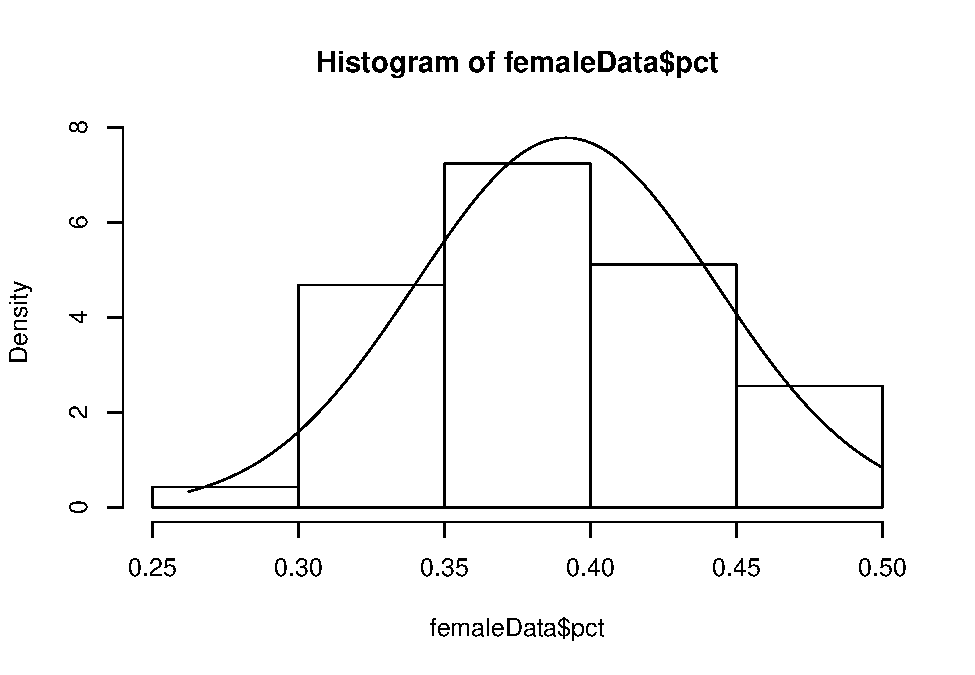
\includegraphics[width=0.5\linewidth]{matstatproblems20-21_files/figure-latex/unnamed-chunk-20-1}
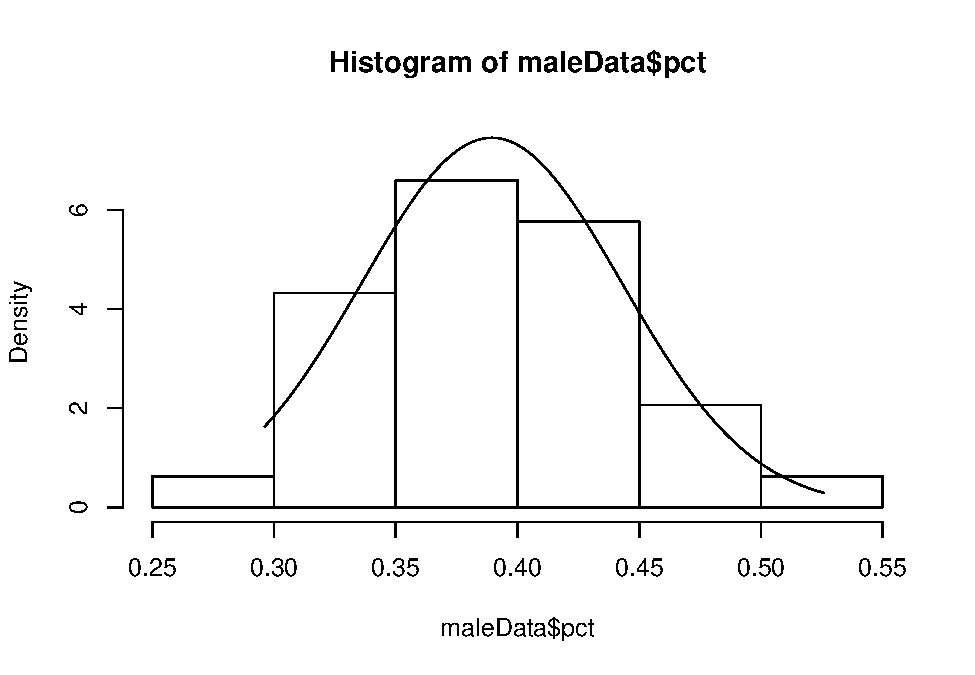
\includegraphics[width=0.5\linewidth]{matstatproblems20-21_files/figure-latex/unnamed-chunk-20-2}

which also doesn't provide a cause for concern to our model assumptions.
Getting to the meat of of the modelcontrol, we may introduce qq-plots
for the two datasets

\begin{Shaded}
\begin{Highlighting}[]
\KeywordTok{qqnorm}\NormalTok{(femaleData}\OperatorTok{$}\NormalTok{pct, }\DataTypeTok{main =} \StringTok{"Female QQ Plot"}\NormalTok{)}
\KeywordTok{abline}\NormalTok{(}\KeywordTok{mean}\NormalTok{(femaleData}\OperatorTok{$}\NormalTok{pct),}\KeywordTok{sd}\NormalTok{(femaleData}\OperatorTok{$}\NormalTok{pct))}

\KeywordTok{qqnorm}\NormalTok{(maleData}\OperatorTok{$}\NormalTok{pct, }\DataTypeTok{main =} \StringTok{"Male QQ Plot"}\NormalTok{)}
\KeywordTok{abline}\NormalTok{(}\KeywordTok{mean}\NormalTok{(maleData}\OperatorTok{$}\NormalTok{pct),}\KeywordTok{sd}\NormalTok{(maleData}\OperatorTok{$}\NormalTok{pct))}
\end{Highlighting}
\end{Shaded}

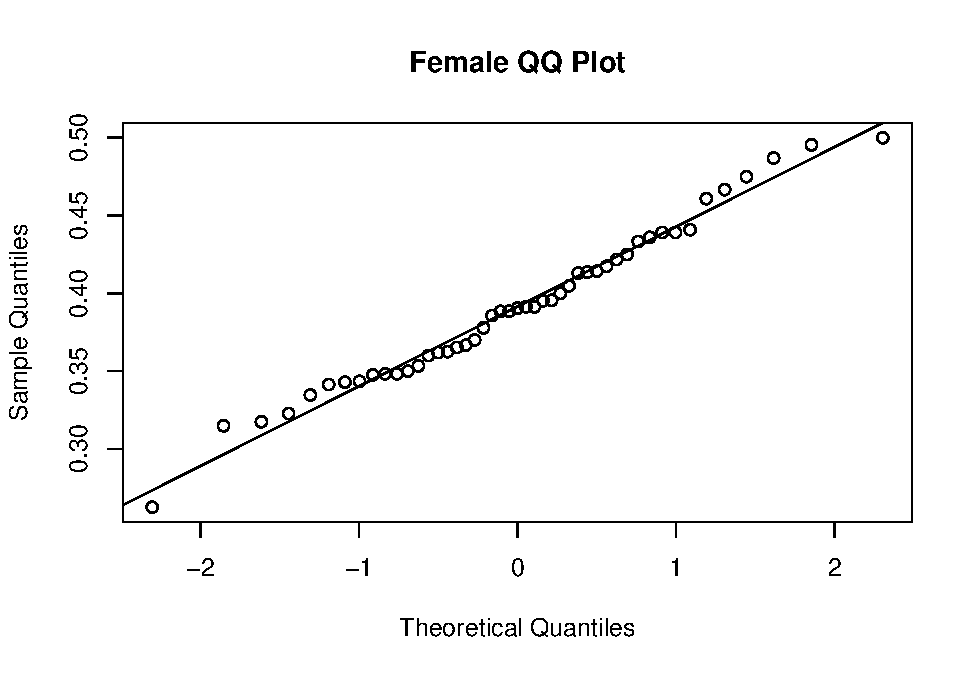
\includegraphics[width=0.5\linewidth]{matstatproblems20-21_files/figure-latex/unnamed-chunk-21-1}
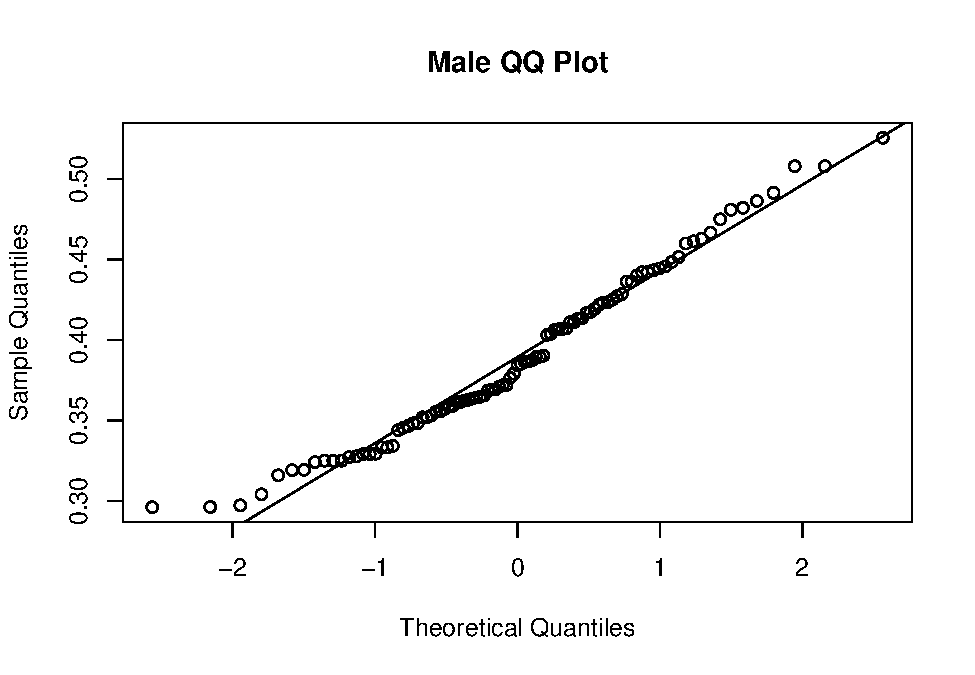
\includegraphics[width=0.5\linewidth]{matstatproblems20-21_files/figure-latex/unnamed-chunk-21-2}

Heed that in both plots, the data seems to hug the empirical line rather
well, thus providing no immediate refutiation of
\texttt{femaleData\$pct} or \texttt{maleData\$pct} being normally
distributed.

\hypertarget{section-12}{%
\paragraph{\texorpdfstring{\textbf{4.}}{4.}}\label{section-12}}

Looking through \texttt{t.test} we may note that a \(95\%\) confidence
interval for the expected difference bewteen \texttt{femaleData\$pct}
and \texttt{maleData\$pct} may be obtained through

\begin{Shaded}
\begin{Highlighting}[]
\KeywordTok{t.test}\NormalTok{(femaleData}\OperatorTok{$}\NormalTok{pct, maleData}\OperatorTok{$}\NormalTok{pct, }\DataTypeTok{paired =}\NormalTok{ F, }\DataTypeTok{var.equal =}\NormalTok{ T)}
\end{Highlighting}
\end{Shaded}

\begin{verbatim}
## 
##  Two Sample t-test
## 
## data:  femaleData$pct and maleData$pct
## t = 0.21935, df = 142, p-value = 0.8267
## alternative hypothesis: true difference in means is not equal to 0
## 95 percent confidence interval:
##  -0.01648249  0.02059684
## sample estimates:
## mean of x mean of y 
## 0.3915119 0.3894547
\end{verbatim}

noting that we have specified that we are not dealing with a paired two
sample - we assume independence between the two groups of female, male
data respectively. - Someplace we find a paired analysis is in
drugtrials with the groupings ``before taking drug'' and ``after taking
drug''. As we sample twice from each person, a rather stark dependence
between the samples occures, as people are rather non-independent of
themselves.

We also include \texttt{var.equal\ =\ T}, thus telling

\includegraphics[width=\textwidth,height=0.16667in]{R_logo.png} that we
assume variance homogeneity between the two samples.

Note that we may extract the confidence interval via

\begin{Shaded}
\begin{Highlighting}[]
\NormalTok{KI <-}\StringTok{ }\KeywordTok{as.numeric}\NormalTok{(}\KeywordTok{t.test}\NormalTok{(femaleData}\OperatorTok{$}\NormalTok{pct, maleData}\OperatorTok{$}\NormalTok{pct, }\DataTypeTok{paired =}\NormalTok{ F, }\DataTypeTok{var.equal =}\NormalTok{ T)[[}\DecValTok{4}\NormalTok{]])}
\NormalTok{KI}
\end{Highlighting}
\end{Shaded}

\begin{verbatim}
## [1] -0.01648249  0.02059684
\end{verbatim}

\begin{Shaded}
\begin{Highlighting}[]
\NormalTok{lKI <-}\StringTok{ }\NormalTok{KI[}\DecValTok{1}\NormalTok{]}
\NormalTok{uKI <-}\StringTok{ }\NormalTok{KI[}\DecValTok{2}\NormalTok{]}
\end{Highlighting}
\end{Shaded}

Note that as \(0\) is firmly placed in the confidence interval, there is
not immidiately any evidence to say that there is a percentagewise
difference in \texttt{heartweight/bodyweight} between male and female
cats.

\hypertarget{section-13}{%
\paragraph{\texorpdfstring{\textbf{5.}}{5.}}\label{section-13}}

Having looked at \texttt{?confint} we may use the requested commands;

\begin{Shaded}
\begin{Highlighting}[]
\NormalTok{fit <-}\StringTok{ }\KeywordTok{lm}\NormalTok{ (pct }\OperatorTok{~}\StringTok{ }\NormalTok{Sex, }\DataTypeTok{data=}\NormalTok{cats)}
\KeywordTok{summary}\NormalTok{(fit)}
\end{Highlighting}
\end{Shaded}

\begin{verbatim}
## 
## Call:
## lm(formula = pct ~ Sex, data = cats)
## 
## Residuals:
##       Min        1Q    Median        3Q       Max 
## -0.129012 -0.038876 -0.003071  0.034442  0.136186 
## 
## Coefficients:
##              Estimate Std. Error t value Pr(>|t|)    
## (Intercept)  0.391512   0.007697  50.863   <2e-16 ***
## SexM        -0.002057   0.009379  -0.219    0.827    
## ---
## Signif. codes:  0 '***' 0.001 '**' 0.01 '*' 0.05 '.' 0.1 ' ' 1
## 
## Residual standard error: 0.05277 on 142 degrees of freedom
## Multiple R-squared:  0.0003387,  Adjusted R-squared:  -0.006701 
## F-statistic: 0.04811 on 1 and 142 DF,  p-value: 0.8267
\end{verbatim}

\begin{Shaded}
\begin{Highlighting}[]
\KeywordTok{confint}\NormalTok{(fit)}
\end{Highlighting}
\end{Shaded}

\begin{verbatim}
##                   2.5 %     97.5 %
## (Intercept)  0.37629566 0.40672807
## SexM        -0.02059684 0.01648249
\end{verbatim}

We may then for example extract the residual standard error through

\begin{Shaded}
\begin{Highlighting}[]
\NormalTok{rstderr <-}\StringTok{ }\KeywordTok{sqrt}\NormalTok{(}\KeywordTok{deviance}\NormalTok{(fit)}\OperatorTok{/}\KeywordTok{df.residual}\NormalTok{(fit))}
\end{Highlighting}
\end{Shaded}

\begin{verbatim}
## [1] 0.05277038
\end{verbatim}

\begin{Shaded}
\begin{Highlighting}[]
\NormalTok{rstderr}\OperatorTok{^}\DecValTok{2}
\end{Highlighting}
\end{Shaded}

\begin{verbatim}
## [1] 0.002784713
\end{verbatim}

\hypertarget{section-14}{%
\paragraph{\texorpdfstring{\textbf{6.}}{6.}}\label{section-14}}

For \(Z_1,\ldots,Z_{144}\) being the stochastic variables representing
\texttt{pct} for the 144 cats, we have assumed
\(E(Z_i)=\mu_1,\,E(Z_j)=\mu_2\) for \(i=1,\ldots,97,\,j=98,\ldots,144\)
respectively representing the male and female cats. We may proceed as
with HS2.6 as we endevour to write a designmatrix \(C\) such that for
\(\eta:=\left({E(Z_1),\ldots,E(Z_{144})}\right)^T\equiv\left({\mu_1,\ldots,\mu_1,\mu_2,\ldots,\mu_2}\right)\)

\[
\eta=C\begin{pmatrix}
\mu_1\\
\mu_2
\end{pmatrix}.
\] Consequently, as
\(\eta\in M_{144,1}(\mathbb{R}),\,\left({\mu_1, \mu_2}\right)^T\in M_{2,1}(\mathbb{R}),\)
we will by matrix multiplication need to have
\(C\in M_{144,2}(\mathbb{R}),\) and in particular for \begin{align*}
C\begin{pmatrix}
\mu_1\\
\mu_2
\end{pmatrix}
\overset{\swarrow}{\equiv}
\begin{pmatrix}
c_{1,1} & c_{1,2} \\
c_{2,1} & c_{2,2} \\
\vdots & \vdots \\
c_{144,1} & c_{144,2}
\end{pmatrix}\begin{pmatrix}
\mu_1\\
\mu_2
\end{pmatrix}&\overset{\swarrow}{=}
\begin{pmatrix}
c_{1,1}\mu_1 + c_{1,2}\mu_2 \\
c_{2,1}\mu_1 + c_{2,2}\mu_2 \\
\vdots \\
c_{144,1}\mu_1 + c_{144,2}\mu_2 
\end{pmatrix}\overset{\searrow}{=}\begin{pmatrix}
\mu_1\\
\vdots\\
\mu_1\\
\mu_2\\
\vdots\\
\mu_2
\end{pmatrix}\overset{\searrow}{\equiv}\eta\\
&\Leftrightarrow\\
c_{i,1}\equiv 1_{\left\{{1,\ldots,97}\right\}}(i)&,\,\,c_{i,2}=1_{\left\{{98,\ldots,144}\right\}}(i)\\
&\Leftrightarrow\\
C&=\begin{pmatrix}
1 & 0 \\
\vdots & \vdots \\
1 & 0 \\
0 & 1 \\
\vdots & \vdots \\
0 & 1
\end{pmatrix}
\end{align*}

\hypertarget{hs-4}{%
\subsection{HS 4}\label{hs-4}}

\hypertarget{section-15}{%
\paragraph{\texorpdfstring{\textbf{1.}}{1.}}\label{section-15}}

\hypertarget{section-16}{%
\paragraph{\texorpdfstring{\textbf{2.}}{2.}}\label{section-16}}

\hypertarget{section-17}{%
\paragraph{\texorpdfstring{\textbf{3.}}{3.}}\label{section-17}}

\hypertarget{hs-5}{%
\subsection{HS 5}\label{hs-5}}

\hypertarget{section-18}{%
\paragraph{\texorpdfstring{\textbf{1.}}{1.}}\label{section-18}}

\hypertarget{section-19}{%
\paragraph{\texorpdfstring{\textbf{2.}}{2.}}\label{section-19}}

\hypertarget{section-20}{%
\paragraph{\texorpdfstring{\textbf{3.}}{3.}}\label{section-20}}

\hypertarget{section-21}{%
\paragraph{\texorpdfstring{\textbf{4.}}{4.}}\label{section-21}}

\hypertarget{section-22}{%
\paragraph{\texorpdfstring{\textbf{5.}}{5.}}\label{section-22}}

\hypertarget{hs-6}{%
\subsection{HS 6}\label{hs-6}}

\hypertarget{section-23}{%
\paragraph{\texorpdfstring{\textbf{1.}}{1.}}\label{section-23}}

Note that for \(X_1,...,X_{10} \sim\mathcal{N}(0,1),\) we may, for
example by NRH problem 1.1, convolution results, or C9.46 in EH (MatStat
Bind 2) conclude regarding the desired distribution. Define in
accordance with C9.46
\(C:=\frac{1}{n}\left({1,\ldots,1}\right)\in\mathbb{R}^{1\times10},\,X:=\left({X_1,\ldots,X_{10}}\right)^T\)
that
\(\overline{X}\equiv\frac{1}{n}\sum_{i=1}^{n}{X_i}\equiv CX \sim \mathcal{N}_1(C\cdot0,CIC^T)=\mathcal{N}_1(0,\frac{1}{n^2}n)=\mathcal{N_1}(0,\frac{1}{n}),\)
which is also in accordance with the result reached in NRH1.1.

\hypertarget{section-24}{%
\paragraph{\texorpdfstring{\textbf{2.}}{2.}}\label{section-24}}

We may test this result through \texttt{gent} number of simulations of
\(10\) outcomes of \(\mathcal{N}(0,1),\) that we will be averaging over;

\begin{Shaded}
\begin{Highlighting}[]
\NormalTok{n<-}\DecValTok{10}
\NormalTok{gent <-}\StringTok{ }\DecValTok{5}\OperatorTok{*}\DecValTok{10}\OperatorTok{^}\DecValTok{3}
\NormalTok{gns <-}\StringTok{ }\KeywordTok{rep}\NormalTok{(}\OtherTok{NA}\NormalTok{,gent)}

\ControlFlowTok{for}\NormalTok{ (i }\ControlFlowTok{in} \DecValTok{1}\OperatorTok{:}\NormalTok{gent) \{}
\NormalTok{  X<-}\KeywordTok{rnorm}\NormalTok{(n,}\DecValTok{0}\NormalTok{,}\DecValTok{1}\NormalTok{)}
\NormalTok{  gns[i] =}\StringTok{ }\DecValTok{1}\OperatorTok{/}\NormalTok{n}\OperatorTok{*}\KeywordTok{sum}\NormalTok{(X)}
\NormalTok{\}}

\KeywordTok{hist}\NormalTok{(gns, }\DataTypeTok{prob =}\NormalTok{ T, }\DataTypeTok{ylim =} \KeywordTok{c}\NormalTok{(}\FloatTok{0.0}\NormalTok{,}\FloatTok{1.3}\NormalTok{))}
\NormalTok{f<-}\StringTok{ }\ControlFlowTok{function}\NormalTok{(x) }\KeywordTok{dnorm}\NormalTok{(x,}\DataTypeTok{mean=}\DecValTok{0}\NormalTok{,}\DataTypeTok{sd=}\DecValTok{1}\OperatorTok{/}\KeywordTok{sqrt}\NormalTok{(n)) }
\KeywordTok{plot}\NormalTok{(f,}\OperatorTok{-}\DecValTok{1}\NormalTok{,}\DecValTok{1}\NormalTok{,}\DataTypeTok{add=}\NormalTok{T)}
\end{Highlighting}
\end{Shaded}

\begin{center}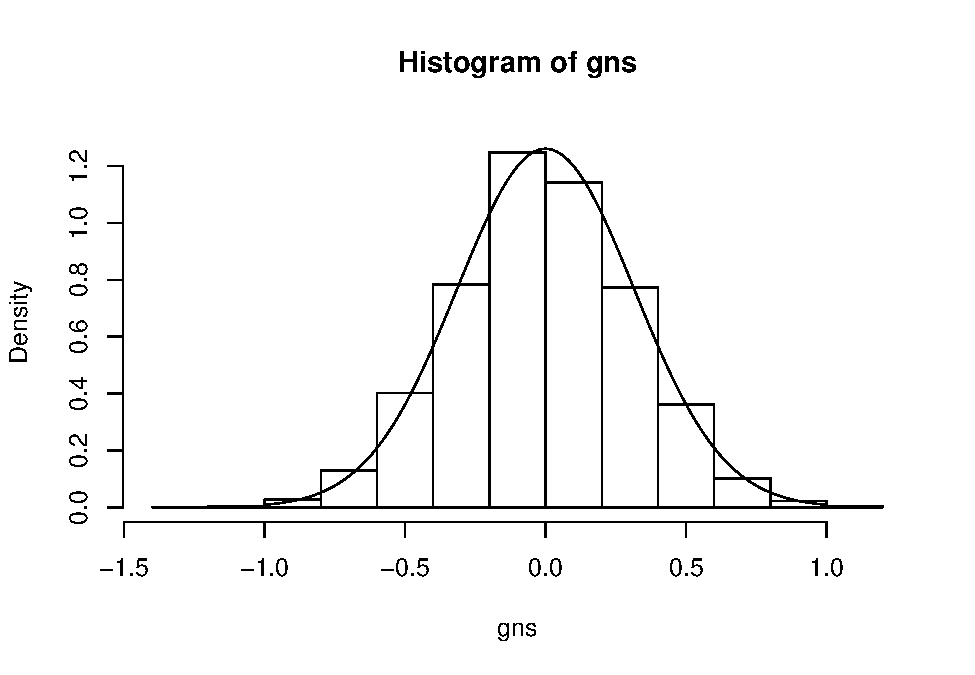
\includegraphics{matstatproblems20-21_files/figure-latex/unnamed-chunk-27-1} \end{center}

Note also that we might we might create a QQ-plot for the data;

\begin{Shaded}
\begin{Highlighting}[]
\KeywordTok{qqnorm}\NormalTok{(gns)}
\KeywordTok{abline}\NormalTok{(}\DecValTok{0}\NormalTok{,}\DecValTok{1}\OperatorTok{/}\KeywordTok{sqrt}\NormalTok{(n))}
\end{Highlighting}
\end{Shaded}

\begin{center}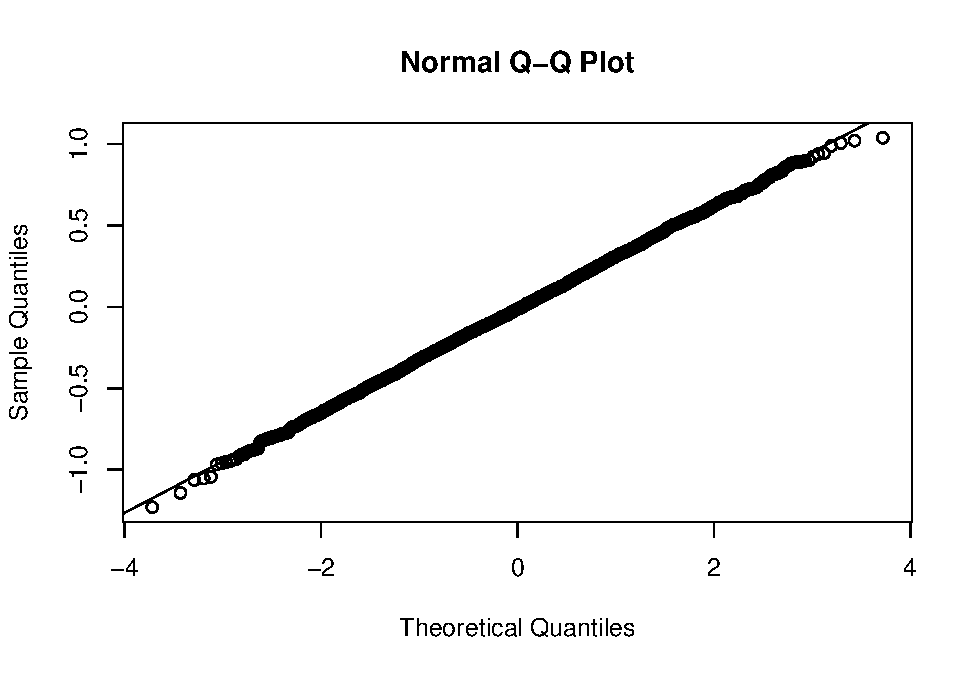
\includegraphics{matstatproblems20-21_files/figure-latex/unnamed-chunk-28-1} \end{center}

for which we see that by Introduktion til Statistik p.~68, everything is
as it should be.

\hypertarget{section-25}{%
\paragraph{\texorpdfstring{\textbf{3.}}{3.}}\label{section-25}}

For each outcome of \(X_1,\ldots,X_{10}\) as \(x_1,\ldots,x_{10},\)
denote by \(x_{(1)}\leq x_{(2)}\leq\ldots\leq x_{(10)}\) the ordering of
the outcomes. As such the median \(\widehat{X},\) of
\(X_1,\ldots,X_{10}\) will equal to \(\frac{x_{(5)}+x_{(6)}}{2},\) and
can be calculated with \texttt{median}

\includegraphics[width=\textwidth,height=0.16667in]{R_logo.png}-command.

So, lets reimplement the above method;

\begin{Shaded}
\begin{Highlighting}[]
\NormalTok{med<-}\KeywordTok{rep}\NormalTok{(}\OtherTok{NA}\NormalTok{,gent)}
\ControlFlowTok{for}\NormalTok{ (i }\ControlFlowTok{in} \DecValTok{1}\OperatorTok{:}\NormalTok{gent) \{}
\NormalTok{   X <-}\StringTok{ }\KeywordTok{rnorm}\NormalTok{(n, }\DecValTok{0}\NormalTok{, }\DecValTok{1}\NormalTok{)}
\NormalTok{   med[i] <-}\StringTok{ }\KeywordTok{median}\NormalTok{(X)}
\NormalTok{\}}
\end{Highlighting}
\end{Shaded}

\begin{Shaded}
\begin{Highlighting}[]
\KeywordTok{hist}\NormalTok{(med, }\DataTypeTok{prob=}\OtherTok{TRUE}\NormalTok{, }\DataTypeTok{ylim =} \KeywordTok{c}\NormalTok{(}\FloatTok{0.0}\NormalTok{,}\FloatTok{1.25}\NormalTok{)) }\CommentTok{# Normeret histogram}
\NormalTok{f <-}\StringTok{ }\ControlFlowTok{function}\NormalTok{(x) }\KeywordTok{dnorm}\NormalTok{(x, }\DataTypeTok{mean=}\DecValTok{0}\NormalTok{, }\DataTypeTok{sd=}\DecValTok{1}\OperatorTok{/}\KeywordTok{sqrt}\NormalTok{(n))}
\KeywordTok{plot}\NormalTok{(f,}\OperatorTok{-}\DecValTok{1}\NormalTok{,}\DecValTok{1}\NormalTok{,}\DataTypeTok{add=}\OtherTok{TRUE}\NormalTok{)}
\end{Highlighting}
\end{Shaded}

\begin{center}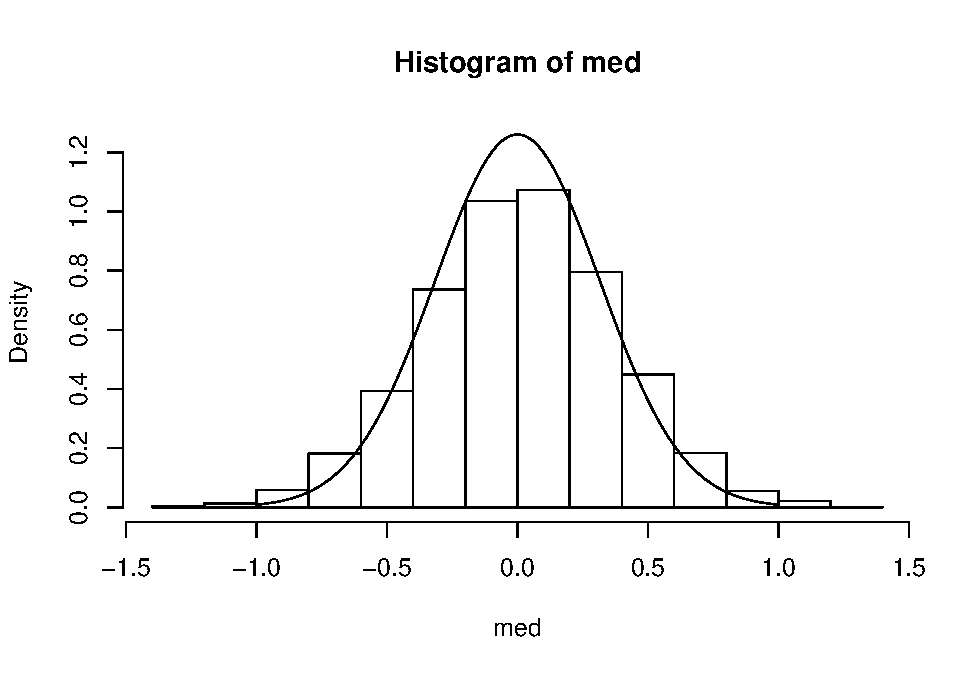
\includegraphics{matstatproblems20-21_files/figure-latex/unnamed-chunk-31-1} \end{center}

\begin{Shaded}
\begin{Highlighting}[]
\CommentTok{#Den tegnede tæthed passer vist ikke helt, idet den designerede tæthed lader til at være mere sammentrykket (højere modus) end histogrammet}
\KeywordTok{hist}\NormalTok{(med, }\DataTypeTok{prob=}\OtherTok{TRUE}\NormalTok{, }\DataTypeTok{ylim =} \KeywordTok{c}\NormalTok{(}\FloatTok{0.0}\NormalTok{,}\FloatTok{1.25}\NormalTok{))}
\NormalTok{f_}\DecValTok{2}\NormalTok{<-}\ControlFlowTok{function}\NormalTok{(x) }\KeywordTok{dnorm}\NormalTok{(x, }\DataTypeTok{mean=} \DecValTok{0}\NormalTok{, }\DataTypeTok{sd =} \KeywordTok{sd}\NormalTok{(med))}
\CommentTok{#Med den empiriske lader det til at gå lidt bedre.}
\KeywordTok{plot}\NormalTok{(f_}\DecValTok{2}\NormalTok{,}\OperatorTok{-}\FloatTok{1.2}\NormalTok{,}\FloatTok{1.2}\NormalTok{,}\DataTypeTok{add =}\NormalTok{ T)}
\end{Highlighting}
\end{Shaded}

\begin{center}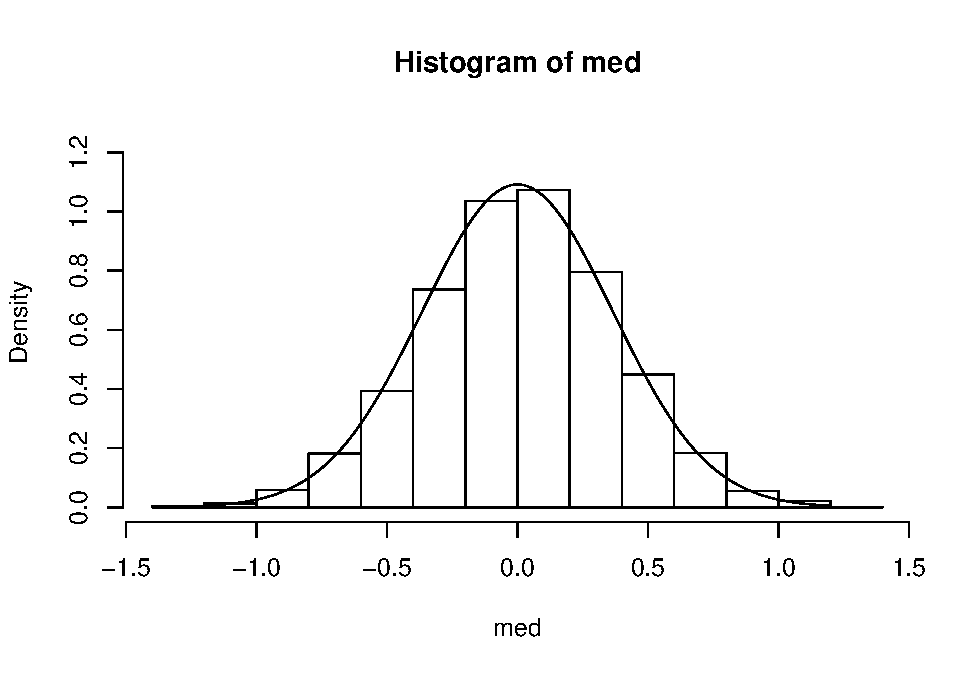
\includegraphics{matstatproblems20-21_files/figure-latex/unnamed-chunk-31-2} \end{center}

\begin{Shaded}
\begin{Highlighting}[]
\KeywordTok{qqnorm}\NormalTok{(med)}
\CommentTok{#qqline(med)}
\KeywordTok{mean}\NormalTok{(med)}
\end{Highlighting}
\end{Shaded}

\begin{verbatim}
## [1] 0.01144251
\end{verbatim}

\begin{Shaded}
\begin{Highlighting}[]
\KeywordTok{sd}\NormalTok{(med)}
\end{Highlighting}
\end{Shaded}

\begin{verbatim}
## [1] 0.3652325
\end{verbatim}

\begin{Shaded}
\begin{Highlighting}[]
\KeywordTok{abline}\NormalTok{(}\DecValTok{0}\NormalTok{,}\KeywordTok{sd}\NormalTok{(med))}
\end{Highlighting}
\end{Shaded}

\begin{center}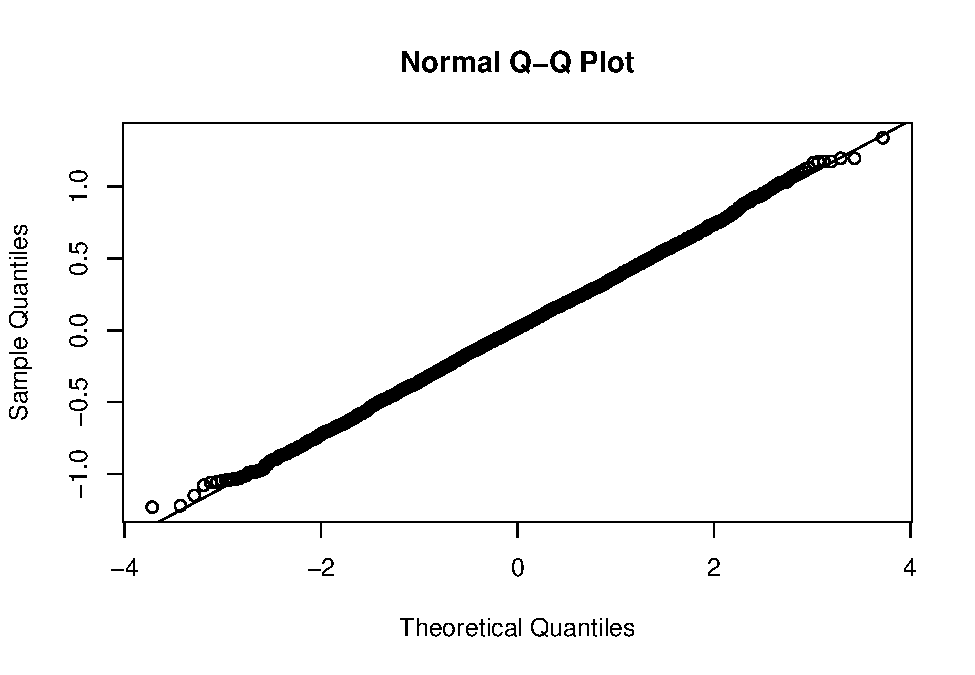
\includegraphics{matstatproblems20-21_files/figure-latex/unnamed-chunk-32-1} \end{center}

With \texttt{mean(med)=} 0.0114425 and \texttt{sd(med)=} 0.3652325, it
seems reasonable by the QQ-plot to assume that the median is going to be
distributed approx. as \(\mathcal{N}(0,0.1333948).\)

Comparing the estimates for the variance of \(\overline{X}\) and
\(\widehat{X}\) we see

\begin{Shaded}
\begin{Highlighting}[]
\KeywordTok{var}\NormalTok{(gns)}
\end{Highlighting}
\end{Shaded}

\begin{verbatim}
## [1] 0.1001461
\end{verbatim}

\begin{Shaded}
\begin{Highlighting}[]
\KeywordTok{var}\NormalTok{(med)}
\end{Highlighting}
\end{Shaded}

\begin{verbatim}
## [1] 0.1333948
\end{verbatim}

with the variance of the mean generally being a good bit lower than the
variance of the median.

We may do a scatterplot of the mean against the median as follows;

\begin{Shaded}
\begin{Highlighting}[]
\KeywordTok{plot}\NormalTok{(}\DataTypeTok{x =}\NormalTok{ gns, }\DataTypeTok{y =}\NormalTok{ med, }\DataTypeTok{xlim =} \KeywordTok{c}\NormalTok{(}\OperatorTok{-}\FloatTok{1.1}\NormalTok{,}\FloatTok{1.1}\NormalTok{), }\DataTypeTok{ylim =} \KeywordTok{c}\NormalTok{(}\OperatorTok{-}\FloatTok{1.1}\NormalTok{,}\FloatTok{1.1}\NormalTok{))}
\end{Highlighting}
\end{Shaded}

\begin{center}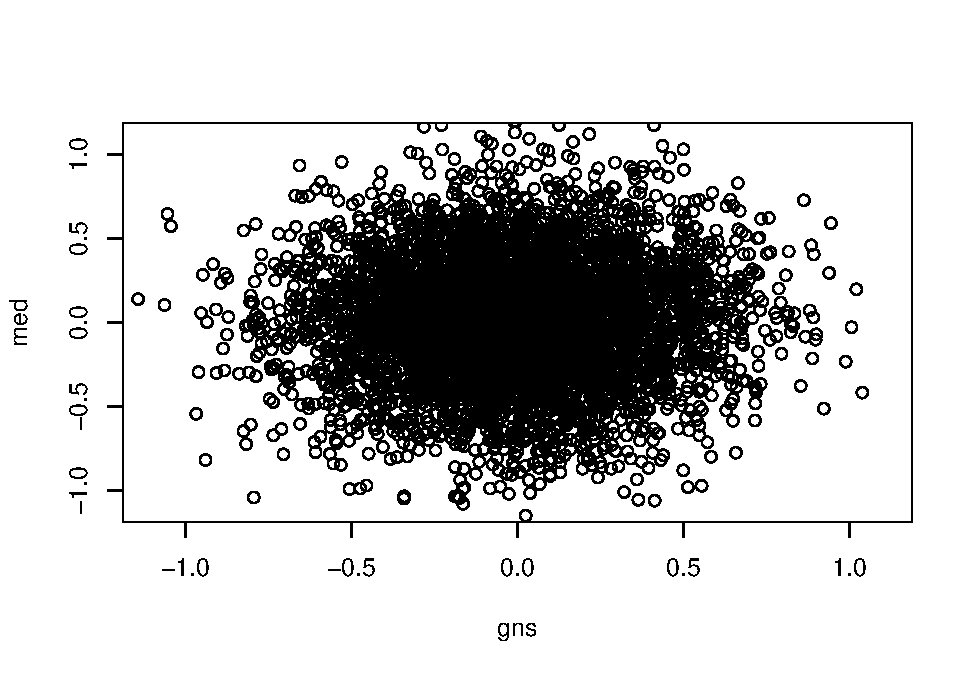
\includegraphics{matstatproblems20-21_files/figure-latex/unnamed-chunk-34-1} \end{center}

We may also use \texttt{?cor} to understand that

\begin{Shaded}
\begin{Highlighting}[]
\KeywordTok{cor}\NormalTok{(gns, med)}
\end{Highlighting}
\end{Shaded}

\begin{verbatim}
## [1] 0.02536134
\end{verbatim}

is to be interpreted as \ldots{}

\hypertarget{hs-7}{%
\subsection{HS 7}\label{hs-7}}

\hypertarget{section-26}{%
\paragraph{\texorpdfstring{\textbf{1.}}{1.}}\label{section-26}}

For \(X\) being a two dimensional stochastic variable with
\[EX=\begin{pmatrix}{1\\0}\end{pmatrix},\,VX=
\begin{pmatrix}
4&4\\
4&16
\end{pmatrix}
\] that as
\(\begin{pmatrix}{1\\0}\end{pmatrix}=EX \equiv E\begin{pmatrix}{X_1\\X_2}\end{pmatrix} \equiv \begin{pmatrix}{EX_1\\EX_2}\end{pmatrix}\)
we get \(EX_1=1,\,EX_2=0.\) In the same way \[
\begin{pmatrix}
4&4\\
4&16
\end{pmatrix}=VX\equiv\begin{pmatrix}
VX_1&cov(X_1,X_2)\\
cov(X_2,X_1)&VX_2
\end{pmatrix}\equiv
\begin{pmatrix}
VX_1&cov(X_1,X_2)\\
cov(X_1,X_2)&VX_2
\end{pmatrix}
\] grants us \(VX_1=4,\,VX_2=16,\,Cov(X_1,X_2)\equiv Cov(X_2,X_1) = 4,\)
and thus \[
Corr(X_1,X_2):=\frac{Cov(X_1,X_2)}{\sqrt{VX_1\,VX_2}}\overset{\cdot}{=}\frac{4}{\sqrt{64}}=\frac{4}{8}=\frac{1}{2}.
\]

\hypertarget{section-27}{%
\paragraph{\texorpdfstring{\textbf{2.}}{2.}}\label{section-27}}

For
\(Y\equiv\begin{pmatrix}{Y_1\\Y_2}\end{pmatrix}:=\begin{pmatrix}{X_1+2\\X_2-X_1+1}\end{pmatrix},\)
we get \[
EY\equiv\begin{pmatrix}{EY_1\\EY_2}\end{pmatrix}\equiv\begin{pmatrix}{E(X_1+2)\\E(X_2-X_1+1)}\end{pmatrix}=\begin{pmatrix}{EX_1+2\\EX_2-EX_1+1}\end{pmatrix}\overset{\cdot}{=}\begin{pmatrix}{1+2\\0-1+1}\end{pmatrix}\equiv\begin{pmatrix}{3\\0}\end{pmatrix}.
\]

In calculating the matrix \(VY\) we may use one of two methods;

\textbf{Method 1: The Direct method}

We also have \[
VY_1\equiv V\left({X_1+2}\right)\overset{\text{MI L16.17}}{=}VX_1=4,
\] and \[
VY_2\equiv V\left({X_2-X_1+1}\right)\overset{\text{MI L16.17}}{=}V\left({X_2-X_1}\right).
\]

\textbf{MI L19.13 expansion}

Let \(Z,Q\) being r.v.r.v.'s variables defined on a common background
space \(\left({\Omega,\mathbb{F}, P}\right).\) If both \(Z,Q\) have
second moments then \[
V\left({Z\pm Q}\right) = VZ + VQ \pm 2Cov(Z,Q)
\]

As both \(X_1,X_2\) have second moment, such that
\(\left({X_1,X_2}\right)\) by MI E19.8 has covariance, we may thus by
the expansion of MI L19.13 above conclude \[
VY_2 = V\left({X_2 - X_1}\right) \overset{\text{L19.13}}{=}VX_2+VX_1-2Cov(X_2,X_1)\underset{\text{MI L19.12}}{\overset{\cdot}{=}} 4+16-2\cdot4=12.
\]

\textbf{MI L19.12 expansion}

Let \(Z,Q,W\) being r.v.r.v.'s variables defined on a common background
space \(\left({\Omega,\mathbb{F}, P}\right).\) If both
\(\left({Z,Q}\right),\,\left({Z,W}\right)\) have covariance then \[
Cov(Z,Q\pm W) = Cov(Q\pm W, Z) = Cov(Q,Z)\pm Cov(W,Z) = Cov(Z,Q)\pm Cov(Z,W)
\]

Having shown above that \(Y_1\) and \(Y_2\) both have finite variance
and thus finite second moments, we may by the MI L19.12 expansion above
conclude \begin{align}

Cov(Y_1,Y_2)&\equiv Cov(X_1+2,X_2-X_1+1)\\
\overset{\text{MI (19.8)}}{=}&Cov(X_1,X_2-X_1)\\
\overset{\text{MI L19.12}}{=}&Cov(X_1,X_2)-Cov(X_1,X_1)\\
\equiv& Cov(X_1,X_2)-VX_1\overset{\cdot}{=}4-4=0

\end{align}

As such we altogether get \[
VY\equiv\begin{pmatrix}4&0\\0&12\end{pmatrix}.
\]

\textbf{Method 2; The Matrix method}

For
\(A:=\begin{pmatrix}1&0\\-1&1\end{pmatrix},\,b:=\begin{pmatrix}{2\\1}\end{pmatrix}\)
note that \(Y=AX+b.\) As such by \begin{align}
VY &\equiv V\left({AX+b}\right)\\
&= V\left({AX}\right)\\
&= AVXA^T\\
&\equiv\begin{pmatrix}1&0\\-1&1\end{pmatrix}\begin{pmatrix}4&4\\4&16\end{pmatrix}\begin{pmatrix}1&-1\\0&1\end{pmatrix}\\
&=\begin{pmatrix}1&0\\-1&1\end{pmatrix}\begin{pmatrix}4&0\\4&12\end{pmatrix}\\
&=\begin{pmatrix}4&0\\0&12\end{pmatrix}
\end{align}

\hypertarget{section-28}{%
\paragraph{\texorpdfstring{\textbf{3.}}{3.}}\label{section-28}}

No we cannot conclude that \(Y_1,Y_2\) are independent just because they
have covariance \(0.\) In general we only have \[
Y_1,Y_2\text{ independent} \Rightarrow Cov(Y_1,Y_2)=0
\] and only (?) in the case in which \(Y_1,Y_2\sim\mathcal{N}\) do we
have \[
Y_1,Y_2\text{ independent and normally distributed} \Leftrightarrow Cov(Y_1,Y_2)=0.
\]

\hypertarget{section-29}{%
\paragraph{\texorpdfstring{\textbf{4.}}{4.}}\label{section-29}}

For
\(A:=\begin{pmatrix}1&0\\-1&1\end{pmatrix},\,b:=\begin{pmatrix}{2\\1}\end{pmatrix}\)
note that \(Y=AX+b,\) as presented in the matrix-method of subproblem2.
By EH K9.46 as \(X\) is now assumed regularly normally distributed, we
will thus have
\(Y\sim\mathcal{N}\left({{A\xi+b},{AVXA^T}}\right)=\mathcal{N}\left({{EY},{VY}}\right)\overset{\cdot}{=}\mathcal{N}\left({{\begin{pmatrix}{3\\0}\end{pmatrix}},{\begin{pmatrix}4&0\\0&12\end{pmatrix}}}\right).\)

\hypertarget{hs-8}{%
\subsection{HS 8}\label{hs-8}}

\hypertarget{section-30}{%
\paragraph{\texorpdfstring{\textbf{1.}}{1.}}\label{section-30}}

Note that we might define new vectors \[
\tilde{p}_0(x):=p_0(x)\equiv1,\quad \tilde{p}_1(x):=p_1(x)\equiv x,\quad \tilde{p}_2(x):=\frac{p_2(x)+p_0(x)}{3}\overset{\cdot}{=}\frac{3x^2-1+1}{3}=x^2,
\] which most definitely span
\(\mathscr{P}_2\equiv\left\{{f:\,\left({-1,1}\right)\rightarrow\mathbb{R}^2|\exists a_0,a_1,a_2\in\mathbb{R},\,f(x)=a_2x^2+a_1*x+a_0}\right\}\),
and as we have transfered from \(\left({p_0,p_1,p_2}\right)\) to
\(\left({\tilde{p}_0,\tilde{p}_1,\tilde{p}_2}\right)\) using only linear
combinations, we will also have that we may therefore conclude that
\(\left({p_0,p_1,p_2}\right)\) must too be a basis for \(\mathscr{P}_2\)

\hypertarget{section-31}{%
\paragraph{\texorpdfstring{\textbf{2.}}{2.}}\label{section-31}}

\begin{Shaded}
\begin{Highlighting}[]
\NormalTok{p0 <-}\StringTok{ }\ControlFlowTok{function}\NormalTok{(x) }\DecValTok{1}
\NormalTok{p1 <-}\StringTok{ }\ControlFlowTok{function}\NormalTok{(x) x}
\NormalTok{p2 <-}\StringTok{ }\ControlFlowTok{function}\NormalTok{(x) }\DecValTok{3}\OperatorTok{*}\NormalTok{x}\OperatorTok{^}\DecValTok{2} \OperatorTok{-}\StringTok{ }\DecValTok{1}
\NormalTok{p12 <-}\StringTok{ }\ControlFlowTok{function}\NormalTok{(x) }\KeywordTok{p1}\NormalTok{(x)}\OperatorTok{*}\KeywordTok{p2}\NormalTok{(x)}
\KeywordTok{integrate}\NormalTok{(p1,}\OperatorTok{-}\DecValTok{1}\NormalTok{,}\DecValTok{1}\NormalTok{)}
\end{Highlighting}
\end{Shaded}

\begin{verbatim}
## 0 with absolute error < 1.1e-14
\end{verbatim}

\begin{Shaded}
\begin{Highlighting}[]
\KeywordTok{integrate}\NormalTok{(p2,}\OperatorTok{-}\DecValTok{1}\NormalTok{,}\DecValTok{1}\NormalTok{)}
\end{Highlighting}
\end{Shaded}

\begin{verbatim}
## -2.775558e-17 with absolute error < 1.7e-14
\end{verbatim}

\begin{Shaded}
\begin{Highlighting}[]
\KeywordTok{integrate}\NormalTok{(p12,}\OperatorTok{-}\DecValTok{1}\NormalTok{,}\DecValTok{1}\NormalTok{)}
\end{Highlighting}
\end{Shaded}

\begin{verbatim}
## 0 with absolute error < 9.2e-15
\end{verbatim}

\hypertarget{section-32}{%
\paragraph{\texorpdfstring{\textbf{3.}}{3.}}\label{section-32}}

Note as described in the problem that as
\(\left\lVert p_0\right\rVert^2=2,\,\left\lVert p_1\right\rVert^2=\frac{2}{3},\,\left\lVert p_2\right\rVert=\frac{8}{5},\)
we may define an orthonormal basis for \(\mathscr{P}_2\) as
\textbackslash begin\{equation\}
e\_0(x):=\textbackslash frac\{1\}\{\textbackslash sqrt\{2\}\},\textbackslash quad
e\_1(x)=\textbackslash sqrt\{\textbackslash frac\{3\}\{2\}\}x,\textbackslash quad
e\_2(x):=\textbackslash sqrt\{\textbackslash frac\{5\}\{8\}\}(3x\^{}2-1),
\textbackslash end\{equation\} in

\includegraphics[width=\textwidth,height=0.16667in]{R_logo.png} with

\begin{Shaded}
\begin{Highlighting}[]
\NormalTok{e0 <-}\StringTok{ }\ControlFlowTok{function}\NormalTok{(x) \{}\DecValTok{1}\OperatorTok{/}\NormalTok{(}\KeywordTok{sqrt}\NormalTok{(}\DecValTok{2}\NormalTok{))\}}
\NormalTok{e1 <-}\StringTok{ }\ControlFlowTok{function}\NormalTok{(x) \{}\KeywordTok{sqrt}\NormalTok{(}\DecValTok{3}\OperatorTok{/}\DecValTok{2}\NormalTok{)}\OperatorTok{*}\NormalTok{x\}}
\NormalTok{e2 <-}\StringTok{ }\ControlFlowTok{function}\NormalTok{(x) \{ }\KeywordTok{sqrt}\NormalTok{(}\DecValTok{5}\OperatorTok{/}\DecValTok{8}\NormalTok{)}\OperatorTok{*}\NormalTok{(}\DecValTok{3}\OperatorTok{*}\NormalTok{x}\OperatorTok{^}\DecValTok{2-1}\NormalTok{)\}}
\end{Highlighting}
\end{Shaded}

Note now, that by C9.28 in EH, we may for
\(Y_0,Y_1,Y_2\sim\mathcal{N}(0,1)\) write any regular normal distributed
random variable \(X\) on \(\mathscr{P}_2\) with precision
\(\left\langle \cdot, \cdot \right\rangle,\) and center \(\xi\) as the
sum \[X:=\sum_{n=0}^{2}{Y_ie_i}+\xi.\] Implementing this in

\includegraphics[width=\textwidth,height=0.16667in]{R_logo.png} we get

\begin{Shaded}
\begin{Highlighting}[]
\NormalTok{xi <-}\StringTok{ }\KeywordTok{c}\NormalTok{(}\DecValTok{0}\NormalTok{,}\DecValTok{0}\NormalTok{,}\DecValTok{0}\NormalTok{)}
\NormalTok{Y_}\DecValTok{0}\NormalTok{ <-}\StringTok{ }\KeywordTok{rnorm}\NormalTok{(}\DecValTok{1}\NormalTok{)}
\NormalTok{Y_}\DecValTok{1}\NormalTok{ <-}\StringTok{ }\KeywordTok{rnorm}\NormalTok{(}\DecValTok{1}\NormalTok{)}
\NormalTok{Y_}\DecValTok{2}\NormalTok{ <-}\StringTok{ }\KeywordTok{rnorm}\NormalTok{(}\DecValTok{1}\NormalTok{)}

\NormalTok{X <-}\StringTok{ }\ControlFlowTok{function}\NormalTok{(x) \{Y_}\DecValTok{0}\OperatorTok{*}\KeywordTok{e0}\NormalTok{(x)}\OperatorTok{+}\NormalTok{Y_}\DecValTok{1}\OperatorTok{*}\KeywordTok{e1}\NormalTok{(x)}\OperatorTok{+}\NormalTok{Y_}\DecValTok{2}\OperatorTok{*}\KeywordTok{e2}\NormalTok{(x) }\OperatorTok{+}\StringTok{ }\NormalTok{xi\}}
\end{Highlighting}
\end{Shaded}

We may also plot the simulated function;

\begin{Shaded}
\begin{Highlighting}[]
\KeywordTok{plot}\NormalTok{(X,}\OperatorTok{-}\DecValTok{1}\NormalTok{,}\DecValTok{1}\NormalTok{)}
\end{Highlighting}
\end{Shaded}

\begin{verbatim}
## Warning in Y_0 * e0(x) + Y_1 * e1(x) + Y_2 * e2(x) + xi: longer object length is
## not a multiple of shorter object length
\end{verbatim}

\begin{center}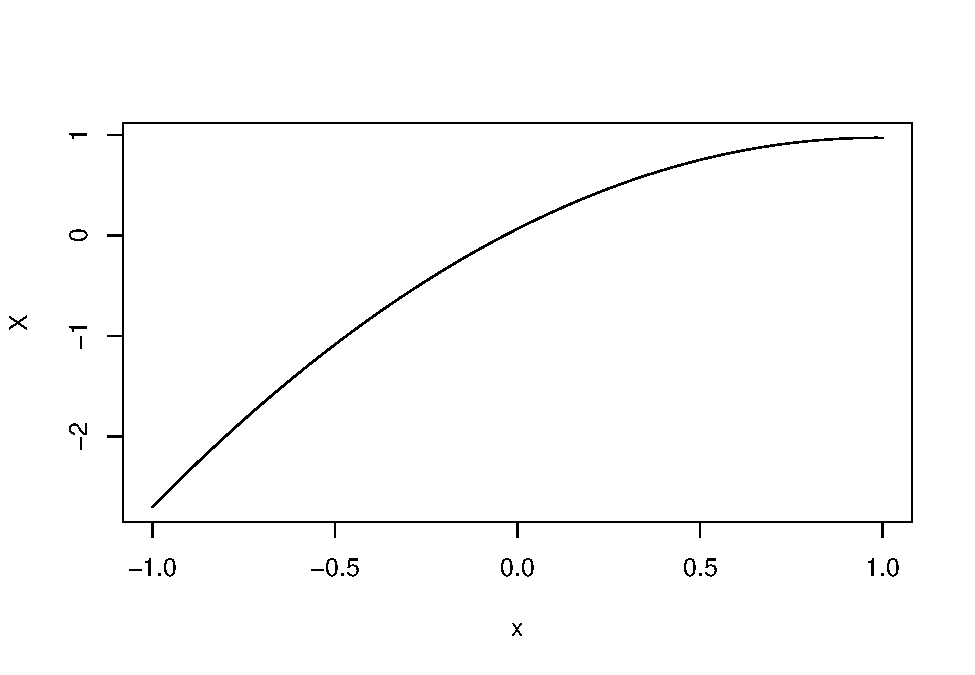
\includegraphics{matstatproblems20-21_files/figure-latex/unnamed-chunk-39-1} \end{center}

\hypertarget{section-33}{%
\paragraph{\texorpdfstring{\textbf{4.}}{4.}}\label{section-33}}

We continue from subproblem 3, but before we do, we will shorten the
construction from 3; Note we may construct a function that simulated our
desired function as follows;

\begin{Shaded}
\begin{Highlighting}[]
\NormalTok{f <-}\StringTok{ }\ControlFlowTok{function}\NormalTok{(x) \{}
\NormalTok{   temp <-}\StringTok{ }\KeywordTok{rnorm}\NormalTok{(}\DecValTok{3}\NormalTok{)}
\NormalTok{   X <-}\StringTok{ }\NormalTok{temp[}\DecValTok{1}\NormalTok{]}\OperatorTok{*}\KeywordTok{e0}\NormalTok{(x)}\OperatorTok{+}\NormalTok{temp[}\DecValTok{2}\NormalTok{]}\OperatorTok{*}\KeywordTok{e1}\NormalTok{(x)}\OperatorTok{+}\NormalTok{temp[}\DecValTok{3}\NormalTok{]}\OperatorTok{*}\KeywordTok{e2}\NormalTok{(x)}
   \KeywordTok{return}\NormalTok{(X)}
\NormalTok{\}}
\end{Highlighting}
\end{Shaded}

As such, we may do the desired simulation as follows

\begin{Shaded}
\begin{Highlighting}[]
\KeywordTok{plot}\NormalTok{(}\DecValTok{0}\NormalTok{,}\DecValTok{0}\NormalTok{, }\DataTypeTok{type=}\StringTok{"n"}\NormalTok{, }\DataTypeTok{xlim=}\KeywordTok{c}\NormalTok{(}\OperatorTok{-}\DecValTok{1}\NormalTok{,}\DecValTok{1}\NormalTok{), }\DataTypeTok{ylim=}\KeywordTok{c}\NormalTok{(}\OperatorTok{-}\DecValTok{3}\NormalTok{,}\DecValTok{3}\NormalTok{), }\DataTypeTok{xlab=}\StringTok{"x"}\NormalTok{, }\DataTypeTok{ylab=}\StringTok{"f(x)"}\NormalTok{)}
\ControlFlowTok{for}\NormalTok{ (i }\ControlFlowTok{in} \DecValTok{1}\OperatorTok{:}\DecValTok{25}\NormalTok{) \{}
\KeywordTok{plot}\NormalTok{(f,}\OperatorTok{-}\DecValTok{1}\NormalTok{,}\DecValTok{1}\NormalTok{, }\DataTypeTok{add=}\OtherTok{TRUE}\NormalTok{) \}}
\end{Highlighting}
\end{Shaded}

\begin{center}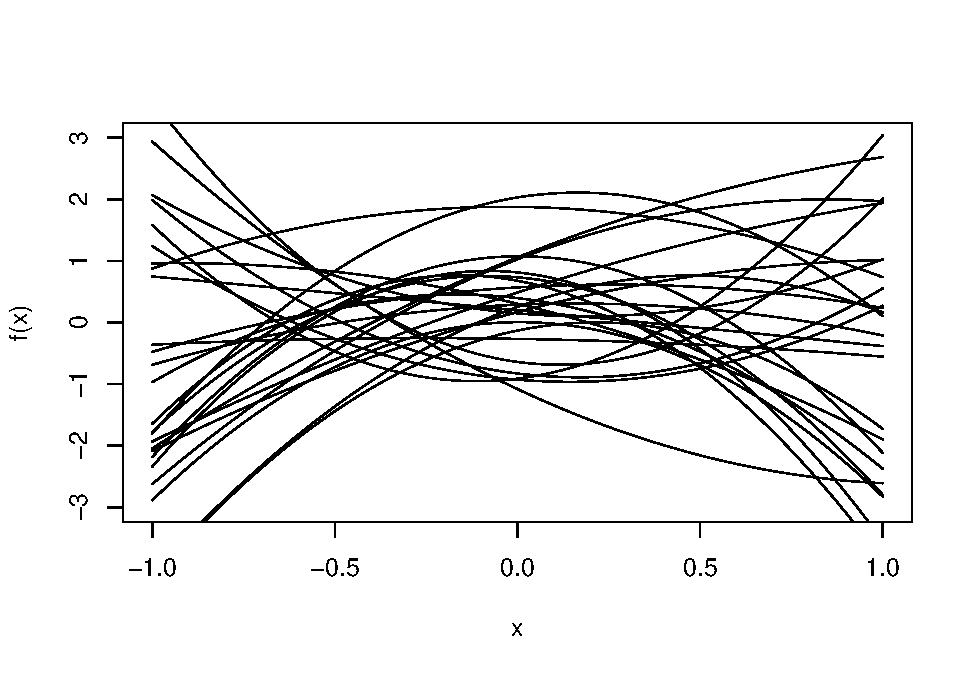
\includegraphics{matstatproblems20-21_files/figure-latex/unnamed-chunk-41-1} \end{center}

\hypertarget{section-34}{%
\paragraph{\texorpdfstring{\textbf{5.}}{5.}}\label{section-34}}

For \(X\) regularly normally distributed on \(\mathscr{P}_2\) with
center \(0\) and precision \(\left\langle \cdot, \cdot \right\rangle\)
Defining \(Z:=t(X),\) as

\hypertarget{hs-9}{%
\subsection{HS 9}\label{hs-9}}

\hypertarget{section-35}{%
\paragraph{\texorpdfstring{\textbf{1.}}{1.}}\label{section-35}}

\hypertarget{section-36}{%
\paragraph{\texorpdfstring{\textbf{2.}}{2.}}\label{section-36}}

\hypertarget{section-37}{%
\paragraph{\texorpdfstring{\textbf{3.}}{3.}}\label{section-37}}

\hypertarget{section-38}{%
\paragraph{\texorpdfstring{\textbf{4.}}{4.}}\label{section-38}}

\hypertarget{section-39}{%
\paragraph{\texorpdfstring{\textbf{5.}}{5.}}\label{section-39}}

\hypertarget{section-40}{%
\paragraph{\texorpdfstring{\textbf{6.}}{6.}}\label{section-40}}

\hypertarget{section-41}{%
\paragraph{\texorpdfstring{\textbf{7.}}{7.}}\label{section-41}}

\hypertarget{hs-10}{%
\subsection{HS 10}\label{hs-10}}

\hypertarget{section-42}{%
\paragraph{\texorpdfstring{\textbf{1.}}{1.}}\label{section-42}}

\hypertarget{section-43}{%
\paragraph{\texorpdfstring{\textbf{2.}}{2.}}\label{section-43}}

\hypertarget{hs-11}{%
\subsection{HS 11}\label{hs-11}}

\hypertarget{section-44}{%
\paragraph{\texorpdfstring{\textbf{1.}}{1.}}\label{section-44}}

Having already completed EH 10.5 in RMD we may copy the assignment of
\(X\) and \(A\) with

\begin{Shaded}
\begin{Highlighting}[]
\NormalTok{A <-}\StringTok{ }\KeywordTok{matrix}\NormalTok{(}\KeywordTok{c}\NormalTok{(}\DecValTok{1}\NormalTok{,}\DecValTok{0}\NormalTok{,}\DecValTok{1}\NormalTok{,}\OperatorTok{-}\DecValTok{1}\NormalTok{,}\DecValTok{1}\NormalTok{,}\OperatorTok{-}\DecValTok{1}\NormalTok{,}\DecValTok{1}\NormalTok{,}\DecValTok{1}\NormalTok{,}\DecValTok{1}\NormalTok{,}\DecValTok{1}\NormalTok{), }\DataTypeTok{nrow =} \DecValTok{5}\NormalTok{, }\DataTypeTok{ncol =} \DecValTok{2}\NormalTok{, }\DataTypeTok{byrow =}\NormalTok{ T) }\CommentTok{#By col is default}
\NormalTok{X <-}\StringTok{ }\KeywordTok{c}\NormalTok{(}\OperatorTok{-}\FloatTok{0.187}\NormalTok{,}\OperatorTok{-}\FloatTok{1.731}\NormalTok{,}\OperatorTok{-}\FloatTok{0.184}\NormalTok{,}\FloatTok{2.252}\NormalTok{,}\FloatTok{1.775}\NormalTok{)}
\end{Highlighting}
\end{Shaded}

\hypertarget{section-45}{%
\paragraph{\texorpdfstring{\textbf{2.}}{2.}}\label{section-45}}

We note that we may reproduce the calculated estimates for
\(\alpha_1,\alpha_2,\sigma\) through \texttt{lm} with

\begin{Shaded}
\begin{Highlighting}[]
\NormalTok{model <-}\StringTok{ }\KeywordTok{lm}\NormalTok{(X}\OperatorTok{~}\NormalTok{A}\DecValTok{-1}\NormalTok{)}
\KeywordTok{model.matrix}\NormalTok{(model)}
\end{Highlighting}
\end{Shaded}

\begin{verbatim}
##   A1 A2
## 1  1  0
## 2  1 -1
## 3  1 -1
## 4  1  1
## 5  1  1
## attr(,"assign")
## [1] 1 1
\end{verbatim}

\begin{Shaded}
\begin{Highlighting}[]
\KeywordTok{summary}\NormalTok{(model)}
\end{Highlighting}
\end{Shaded}

\begin{verbatim}
## 
## Call:
## lm(formula = X ~ A - 1)
## 
## Residuals:
##       1       2       3       4       5 
## -0.5720 -0.6305  0.9165  0.3815 -0.0955 
## 
## Coefficients:
##    Estimate Std. Error t value Pr(>|t|)  
## A1   0.3850     0.3386   1.137   0.3381  
## A2   1.4855     0.3785   3.924   0.0294 *
## ---
## Signif. codes:  0 '***' 0.001 '**' 0.01 '*' 0.05 '.' 0.1 ' ' 1
## 
## Residual standard error: 0.757 on 3 degrees of freedom
## Multiple R-squared:  0.8477, Adjusted R-squared:  0.7461 
## F-statistic: 8.347 on 2 and 3 DF,  p-value: 0.05945
\end{verbatim}

Looking through \texttt{?model.matrix} enlightens us a bit as to the
output of \texttt{model.matrix(model)} Note that we find the estimate
for \(\alpha_1,\,\hat\alpha_1\) under \texttt{{[}A1,Estimate\ Std.{]}},
\(\alpha_2,\,\hat\alpha_2\) under \texttt{{[}A2,Estimate\ Std.{]}} and
the estimate for \(\sigma,\,???\) under
\texttt{Residual\ standard\ error} We may extract these three estimates
with the below commands, noting that

\begin{Shaded}
\begin{Highlighting}[]
\NormalTok{model}\OperatorTok{$}\NormalTok{coefficients[[}\DecValTok{1}\NormalTok{]] }\CommentTok{#alphahat_1}
\end{Highlighting}
\end{Shaded}

\begin{verbatim}
## [1] 0.385
\end{verbatim}

\begin{Shaded}
\begin{Highlighting}[]
\NormalTok{model}\OperatorTok{$}\NormalTok{coefficients[[}\DecValTok{2}\NormalTok{]] }\CommentTok{#alphahat_2}
\end{Highlighting}
\end{Shaded}

\begin{verbatim}
## [1] 1.4855
\end{verbatim}

\begin{Shaded}
\begin{Highlighting}[]
\KeywordTok{summary}\NormalTok{(model)}\OperatorTok{$}\NormalTok{sigma }\CommentTok{#sigmatilde}
\end{Highlighting}
\end{Shaded}

\begin{verbatim}
## [1] 0.7570445
\end{verbatim}

\begin{Shaded}
\begin{Highlighting}[]
\NormalTok{sigmatilde2 <-}\StringTok{ }\NormalTok{(}\KeywordTok{summary}\NormalTok{(model)}\OperatorTok{$}\NormalTok{sigma)}\OperatorTok{^}\DecValTok{2} \CommentTok{#sigmatilde^2}
\end{Highlighting}
\end{Shaded}

\begin{verbatim}
## [1] 0.5731163
\end{verbatim}

\hypertarget{section-46}{%
\paragraph{\texorpdfstring{\textbf{3.}}{3.}}\label{section-46}}

Having checked \texttt{?vcov}, note the output of \texttt{vcov} and
\texttt{solve(t(A)A)}-commands;

\begin{Shaded}
\begin{Highlighting}[]
\KeywordTok{vcov}\NormalTok{(model)}
\end{Highlighting}
\end{Shaded}

\begin{verbatim}
##           A1        A2
## A1 0.1146233 0.0000000
## A2 0.0000000 0.1432791
\end{verbatim}

\begin{Shaded}
\begin{Highlighting}[]
\KeywordTok{solve}\NormalTok{(}\KeywordTok{t}\NormalTok{(A)}\OperatorTok\NormalTok{A)}
\end{Highlighting}
\end{Shaded}

\begin{verbatim}
##      [,1] [,2]
## [1,]  0.2 0.00
## [2,]  0.0 0.25
\end{verbatim}

On an inkling that there ``might'' be a connection between
\texttt{sigmatilde,vcov(model),solve(t(A)\%*\%A)} note that

\begin{Shaded}
\begin{Highlighting}[]
\KeywordTok{solve}\NormalTok{(}\KeywordTok{t}\NormalTok{(A)}\OperatorTok\NormalTok{A)}\OperatorTok{*}\NormalTok{sigmatilde2 }\CommentTok{#Fits rather well with vcov(model)}
\end{Highlighting}
\end{Shaded}

\begin{verbatim}
##           [,1]      [,2]
## [1,] 0.1146233 0.0000000
## [2,] 0.0000000 0.1432791
\end{verbatim}

Referring back to EH 10.5 and the distribution of the MLE mean
\(\hat\alpha\sim\mathcal{N}\left({{\alpha},{\tilde\sigma^2\left({A^TA}\right)^{-1}}}\right),\)
this isn't entirely surprising, when noting the fact that
\texttt{vcov(model)} - by \texttt{?vcov} itself describes its
functionality as;

\emph{Returns the variance-covariance matrix of the main parameters of a
fitted model object. The ``main'' parameters of model correspond to
those returned by coef, and typically do not contain a nuisance scale
parameter (sigma).}

\hypertarget{section-47}{%
\paragraph{\texorpdfstring{\textbf{4.}}{4.}}\label{section-47}}

Referring back to HS2 in which the extraction of standard errors for
estimates based on some linear regression was first carried out, turns
out to give us clues as to the connections.

\begin{Shaded}
\begin{Highlighting}[]
\NormalTok{sealpha_}\DecValTok{1}\NormalTok{ <-}\StringTok{ }\KeywordTok{sqrt}\NormalTok{(}\KeywordTok{diag}\NormalTok{(}\KeywordTok{vcov}\NormalTok{(model)))[[}\DecValTok{1}\NormalTok{]]}
\end{Highlighting}
\end{Shaded}

\begin{verbatim}
## [1] 0.3385606
\end{verbatim}

\begin{Shaded}
\begin{Highlighting}[]
\NormalTok{sealpha_}\DecValTok{2}\NormalTok{ <-}\StringTok{ }\KeywordTok{sqrt}\NormalTok{(}\KeywordTok{diag}\NormalTok{(}\KeywordTok{vcov}\NormalTok{(model)))[[}\DecValTok{2}\NormalTok{]]}
\end{Highlighting}
\end{Shaded}

\begin{verbatim}
## [1] 0.3785222
\end{verbatim}

Note then that \[
SE_{\hat\alpha_1}=\sqrt{\underset{\text{vcov(model)[1,1]}}{\underbrace{\tilde\sigma^2\left({A^TA}\right)^{-1}_{11}}}}\\
SE_{\hat\alpha_2}=\sqrt{\underset{\text{vcov(model)[2,2]}}{\underbrace{\tilde\sigma^2\left({A^TA}\right)^{-1}_{22}}}}
\]

\hypertarget{hs-12}{%
\subsection{HS 12}\label{hs-12}}

\hypertarget{section-48}{%
\paragraph{\texorpdfstring{\textbf{1.}}{1.}}\label{section-48}}

\hypertarget{section-49}{%
\paragraph{\texorpdfstring{\textbf{2.}}{2.}}\label{section-49}}

\hypertarget{hs-13}{%
\subsection{HS 13}\label{hs-13}}

Note that we are running seed 314 throughout this RMD document.

\hypertarget{section-50}{%
\paragraph{\texorpdfstring{\textbf{1.}}{1.}}\label{section-50}}

We may read the data into

\includegraphics[width=\textwidth,height=0.16667in]{R_logo.png} and
define the requested variables with

\begin{Shaded}
\begin{Highlighting}[]
\NormalTok{paddy <-}\StringTok{ }\KeywordTok{read.csv}\NormalTok{(}\StringTok{"paddy.txt"}\NormalTok{, }\DataTypeTok{sep=}\StringTok{""}\NormalTok{) }
\KeywordTok{head}\NormalTok{(paddy)}
\end{Highlighting}
\end{Shaded}

\begin{verbatim}
##   days yield
## 1   16  2508
## 2   18  2518
## 3   20  3304
## 4   22  3423
## 5   24  3057
## 6   26  3190
\end{verbatim}

\begin{Shaded}
\begin{Highlighting}[]
\NormalTok{days <-}\StringTok{ }\NormalTok{paddy}\OperatorTok{$}\NormalTok{days}
\NormalTok{yield <-}\StringTok{ }\NormalTok{paddy}\OperatorTok{$}\NormalTok{yield}
\NormalTok{daysSqr <-}\StringTok{ }\NormalTok{days}\OperatorTok{^}\DecValTok{2}
\NormalTok{kvadreg <-}\StringTok{ }\KeywordTok{lm}\NormalTok{(yield }\OperatorTok{~}\NormalTok{days}\OperatorTok{+}\NormalTok{daysSqr)}
\KeywordTok{summary}\NormalTok{(kvadreg)}
\end{Highlighting}
\end{Shaded}

\begin{verbatim}
## 
## Call:
## lm(formula = yield ~ days + daysSqr)
## 
## Residuals:
##     Min      1Q  Median      3Q     Max 
## -303.96 -118.11   13.86  115.67  319.06 
## 
## Coefficients:
##               Estimate Std. Error t value Pr(>|t|)    
## (Intercept) -1070.3977   617.2527  -1.734    0.107    
## days          293.4829    42.1776   6.958 9.94e-06 ***
## daysSqr        -4.5358     0.6744  -6.726 1.41e-05 ***
## ---
## Signif. codes:  0 '***' 0.001 '**' 0.01 '*' 0.05 '.' 0.1 ' ' 1
## 
## Residual standard error: 203.9 on 13 degrees of freedom
## Multiple R-squared:  0.7942, Adjusted R-squared:  0.7625 
## F-statistic: 25.08 on 2 and 13 DF,  p-value: 3.452e-05
\end{verbatim}

we have made made the regression model as written in EH (11.15). Note
that we may collect estimates of \(\hat\alpha,\,\hat\beta\) and
\(\hat\gamma\) with the code

\begin{Shaded}
\begin{Highlighting}[]
\NormalTok{alphah <-}\StringTok{ }\NormalTok{kvadreg}\OperatorTok{$}\NormalTok{coefficients[[}\DecValTok{1}\NormalTok{]]}
\end{Highlighting}
\end{Shaded}

\begin{verbatim}
## [1] -1070.398
\end{verbatim}

\begin{Shaded}
\begin{Highlighting}[]
\NormalTok{betah <-}\StringTok{ }\NormalTok{kvadreg}\OperatorTok{$}\NormalTok{coefficients[[}\DecValTok{2}\NormalTok{]]}
\end{Highlighting}
\end{Shaded}

\begin{verbatim}
## [1] 293.4829
\end{verbatim}

\begin{Shaded}
\begin{Highlighting}[]
\NormalTok{gammah <-}\StringTok{ }\NormalTok{kvadreg}\OperatorTok{$}\NormalTok{coefficients[[}\DecValTok{3}\NormalTok{]]}
\end{Highlighting}
\end{Shaded}

\begin{verbatim}
## [1] -4.535802
\end{verbatim}

\begin{Shaded}
\begin{Highlighting}[]
\NormalTok{tsigma2 <-}\StringTok{ }\NormalTok{(}\KeywordTok{summary}\NormalTok{(kvadreg)}\OperatorTok{$}\NormalTok{sigma)}\OperatorTok{^}\DecValTok{2}
\end{Highlighting}
\end{Shaded}

\begin{verbatim}
## [1] 41568.34
\end{verbatim}

and that these match the estimates reported in EH Example 11.10.

\hypertarget{section-51}{%
\paragraph{\texorpdfstring{\textbf{2.}}{2.}}\label{section-51}}

We will be plotting the standard residuals against the estimated
(fitted) values for \texttt{yield}, in the same way we did (eg.) in HS2;

\begin{Shaded}
\begin{Highlighting}[]
\NormalTok{fit <-}\StringTok{ }\KeywordTok{fitted}\NormalTok{(kvadreg)}
\NormalTok{rst <-}\StringTok{ }\KeywordTok{rstandard}\NormalTok{(kvadreg)}
\KeywordTok{plot}\NormalTok{(fit, rst, }\DataTypeTok{main =} \StringTok{"(Estimate, Std. Res.)-plot for kvadreg model on paddy"}\NormalTok{, }\DataTypeTok{xlab =} \StringTok{"Estimated (fitted) yield-values (kg/ha)"}\NormalTok{, }\DataTypeTok{ylab =}\StringTok{"Standardized residuals"}\NormalTok{, }\DataTypeTok{ylim =} \KeywordTok{c}\NormalTok{(}\OperatorTok{-}\KeywordTok{max}\NormalTok{(}\FloatTok{3.2}\NormalTok{,}\KeywordTok{max}\NormalTok{(}\KeywordTok{abs}\NormalTok{(rst))), }\KeywordTok{max}\NormalTok{(}\FloatTok{3.2}\NormalTok{,}\KeywordTok{max}\NormalTok{(}\KeywordTok{abs}\NormalTok{(rst)))) ) }\CommentTok{#Largest symmetric interval (around 0) of (-3.2,3.2) or (-largest absolute rst, largest absolute rst)}
\KeywordTok{abline}\NormalTok{(}\DecValTok{0}\NormalTok{,}\DecValTok{0}\NormalTok{)}
\end{Highlighting}
\end{Shaded}

\begin{center}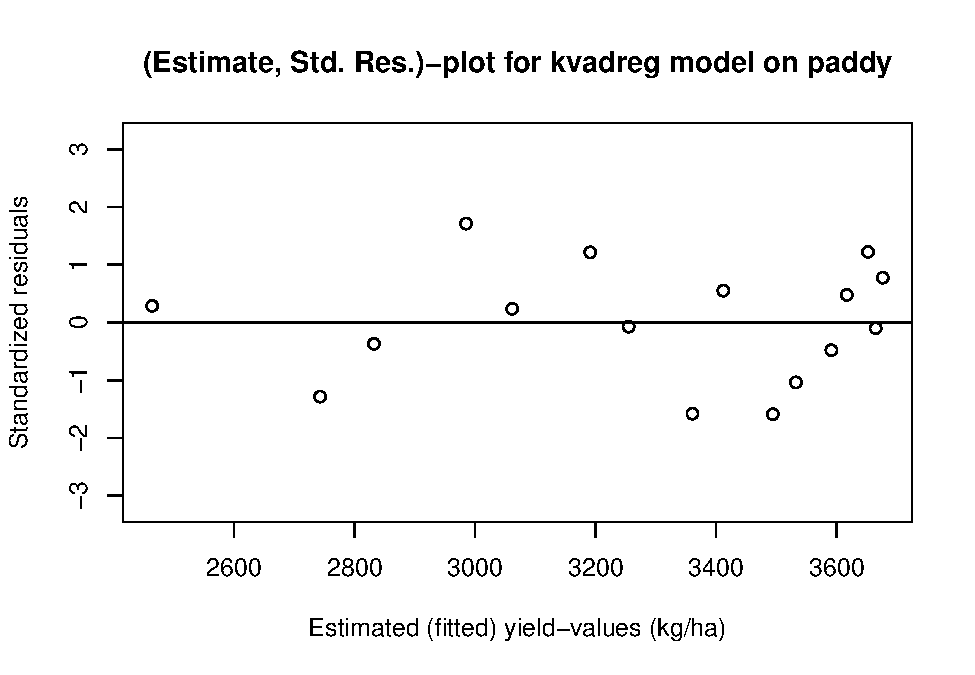
\includegraphics{matstatproblems20-21_files/figure-latex/unnamed-chunk-50-1} \end{center}

Looking at the above plot, we note that if the assumption that the
variance of the yield data is independent of the mean is true, we would
expect that the dispersion of points at region of fitted yield values
would be akin to the dispersion in any other region. If the
``linearity'' assumption of our model were to be true, we would expect
the points to be relatively equally dispersed as \(\mathcal{N}(0,1)\) on
both sides of \(0\) across the fitted values. - ie. that the
standardized residuals are themselves rather \(\mathcal{N}(0,1)\)
distributed.

The plot looks rather respectable on both these fronts, as 1. The (std.)
residual values fall within the interval \(\left({-1.5,1.5}\right),\) as
would be expected of a standard normal distribution. 2. No wierd
``trumpet'', ``quadratic'' or other wierd distortions to the std.
residuals values are present, they seem to keep rather constantly
dispersed around zero within any fitted yield region.

\hypertarget{section-52}{%
\paragraph{\texorpdfstring{\textbf{3.}}{3.}}\label{section-52}}

We may run the requested commands in

\includegraphics[width=\textwidth,height=0.16667in]{R_logo.png},
simulating \(16\) new datapoints from the normal distribution with mean
and variance parameters defined as the empirical parameters of the
original data. The implementation;

\begin{Shaded}
\begin{Highlighting}[]
\NormalTok{xi0 <-}\StringTok{ }\KeywordTok{fitted}\NormalTok{(kvadreg)}
\NormalTok{sigma0 <-}\StringTok{ }\KeywordTok{summary}\NormalTok{(kvadreg)}\OperatorTok{$}\NormalTok{sigma}
\end{Highlighting}
\end{Shaded}

\begin{verbatim}
## [1] 203.8831
\end{verbatim}

\begin{Shaded}
\begin{Highlighting}[]
\NormalTok{simYield <-}\StringTok{ }\KeywordTok{rnorm}\NormalTok{(}\DecValTok{16}\NormalTok{, xi0, sigma0)}
\end{Highlighting}
\end{Shaded}

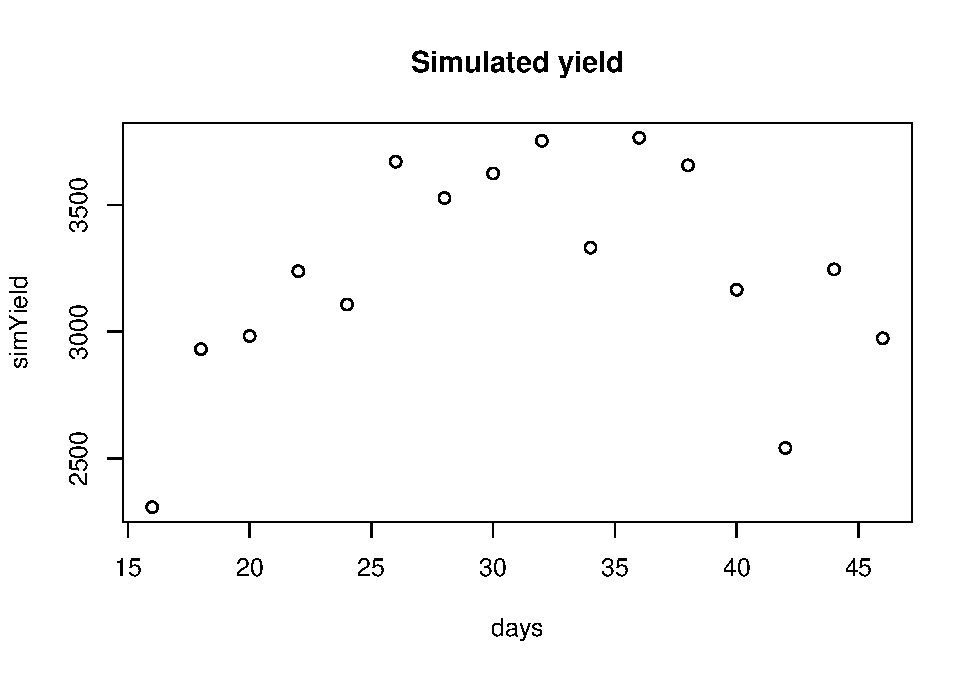
\includegraphics[width=0.5\linewidth]{matstatproblems20-21_files/figure-latex/unnamed-chunk-51-1}
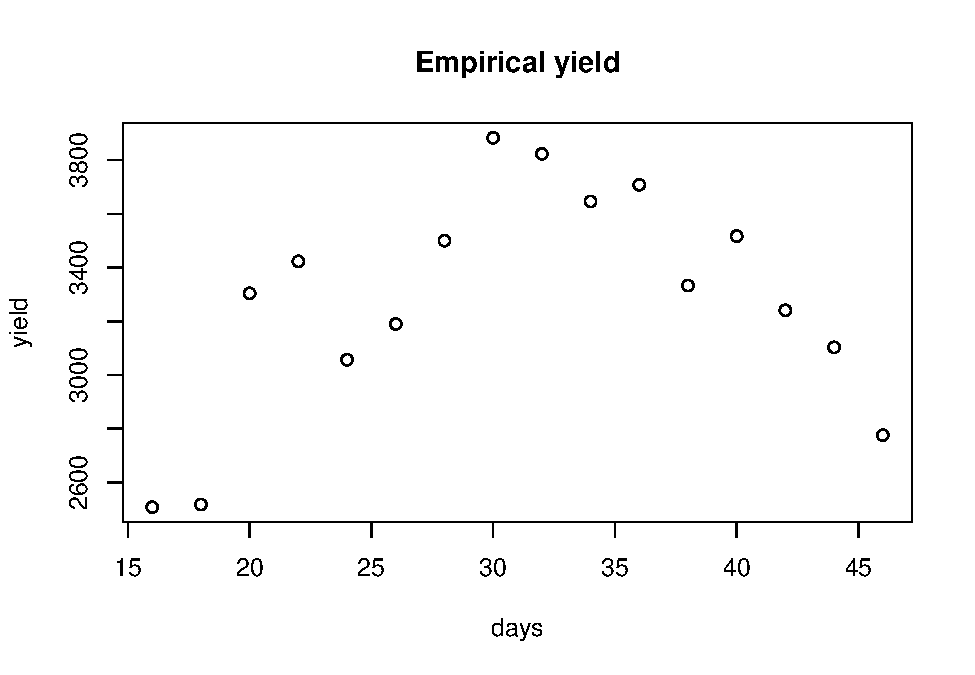
\includegraphics[width=0.5\linewidth]{matstatproblems20-21_files/figure-latex/unnamed-chunk-51-2}

We note that the simulated scatterplot retains a lot of the
characteristics of the original, though it is definitely different to
the original.

\hypertarget{section-53}{%
\paragraph{\texorpdfstring{\textbf{4.}}{4.}}\label{section-53}}

As we did with the original data, we will just as well fit a quadratic
regression model to the simulated data.

\begin{Shaded}
\begin{Highlighting}[]
\NormalTok{yield2 <-}\StringTok{ }\NormalTok{simYield}
\NormalTok{kvadreg2 <-}\StringTok{ }\KeywordTok{lm}\NormalTok{(yield2 }\OperatorTok{~}\StringTok{ }\NormalTok{days}\OperatorTok{+}\NormalTok{daysSqr)}
\NormalTok{alphah2 <-}\StringTok{ }\NormalTok{kvadreg2}\OperatorTok{$}\NormalTok{coefficients[[}\DecValTok{1}\NormalTok{]]}
\end{Highlighting}
\end{Shaded}

\begin{verbatim}
## [1] -868.701
\end{verbatim}

\begin{Shaded}
\begin{Highlighting}[]
\NormalTok{betah2 <-}\StringTok{ }\NormalTok{kvadreg2}\OperatorTok{$}\NormalTok{coefficients[[}\DecValTok{2}\NormalTok{]]}
\end{Highlighting}
\end{Shaded}

\begin{verbatim}
## [1] 279.8275
\end{verbatim}

\begin{Shaded}
\begin{Highlighting}[]
\NormalTok{gammah2 <-}\StringTok{ }\NormalTok{kvadreg2}\OperatorTok{$}\NormalTok{coefficients[[}\DecValTok{3}\NormalTok{]]}
\end{Highlighting}
\end{Shaded}

\begin{verbatim}
## [1] -4.365983
\end{verbatim}

\begin{Shaded}
\begin{Highlighting}[]
\NormalTok{tsigma2_}\DecValTok{2}\NormalTok{ <-}\StringTok{ }\NormalTok{(}\KeywordTok{summary}\NormalTok{(kvadreg2)}\OperatorTok{$}\NormalTok{sigma)}\OperatorTok{^}\DecValTok{2}
\end{Highlighting}
\end{Shaded}

\begin{verbatim}
## [1] 68692.48
\end{verbatim}

We may also create a new std. residual plot for the simulated data

\begin{Shaded}
\begin{Highlighting}[]
\NormalTok{fit2 <-}\StringTok{ }\KeywordTok{fitted}\NormalTok{(kvadreg2)}
\NormalTok{rst2 <-}\StringTok{ }\KeywordTok{rstandard}\NormalTok{(kvadreg2)}
\KeywordTok{plot}\NormalTok{(fit2, rst2, }\DataTypeTok{main =} \StringTok{"(Estimate, Std. Res.)-plot for kvadreg2 model on paddy"}\NormalTok{, }\DataTypeTok{xlab =} \StringTok{"Estimated (fitted) yield-values (kg/ha)"}\NormalTok{, }\DataTypeTok{ylab =}\StringTok{"Standardized residuals"}\NormalTok{, }\DataTypeTok{ylim =} \KeywordTok{c}\NormalTok{(}\OperatorTok{-}\KeywordTok{max}\NormalTok{(}\FloatTok{3.2}\NormalTok{,}\KeywordTok{max}\NormalTok{(}\KeywordTok{abs}\NormalTok{(rst2))), }\KeywordTok{max}\NormalTok{(}\FloatTok{3.2}\NormalTok{,}\KeywordTok{max}\NormalTok{(}\KeywordTok{abs}\NormalTok{(rst2)))) ) }\CommentTok{#Largest symmetric interval (around 0) of (-3.2,3.2) or (-largest absolute rst, largest absolute rst)}
\KeywordTok{abline}\NormalTok{(}\DecValTok{0}\NormalTok{,}\DecValTok{0}\NormalTok{)}
\end{Highlighting}
\end{Shaded}

\begin{center}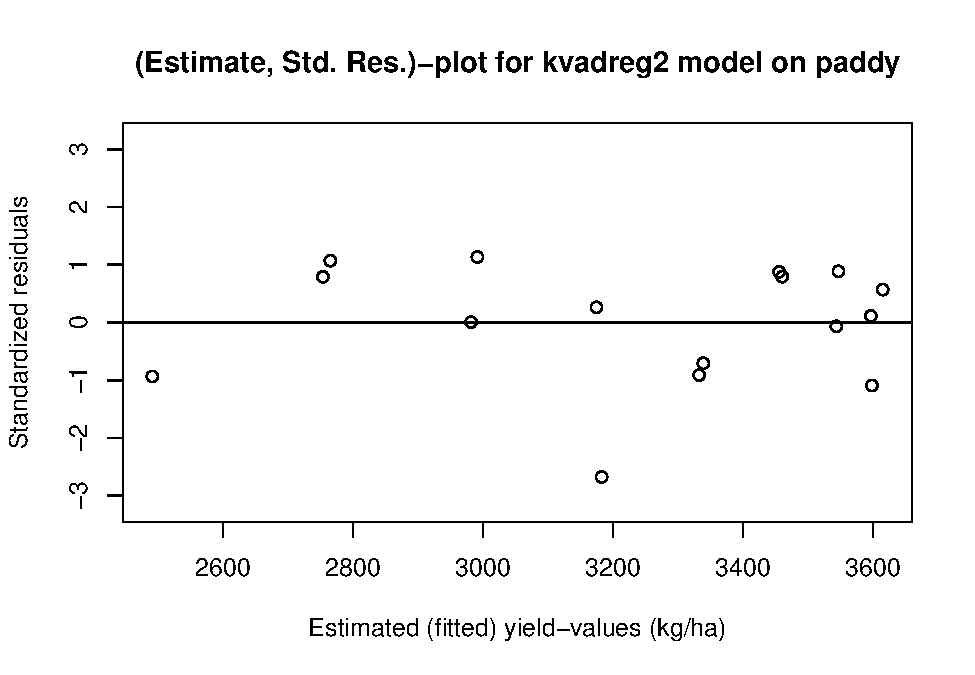
\includegraphics{matstatproblems20-21_files/figure-latex/unnamed-chunk-53-1} \end{center}

Which once again doesn't seem to have much of anything out of the
ordinary.

\hypertarget{section-54}{%
\paragraph{\texorpdfstring{\textbf{5.}}{5.}}\label{section-54}}

We may define a simulation factory function \texttt{Sim}. Do also note
the functionality of the \texttt{par} function with \texttt{?par}

\begin{center}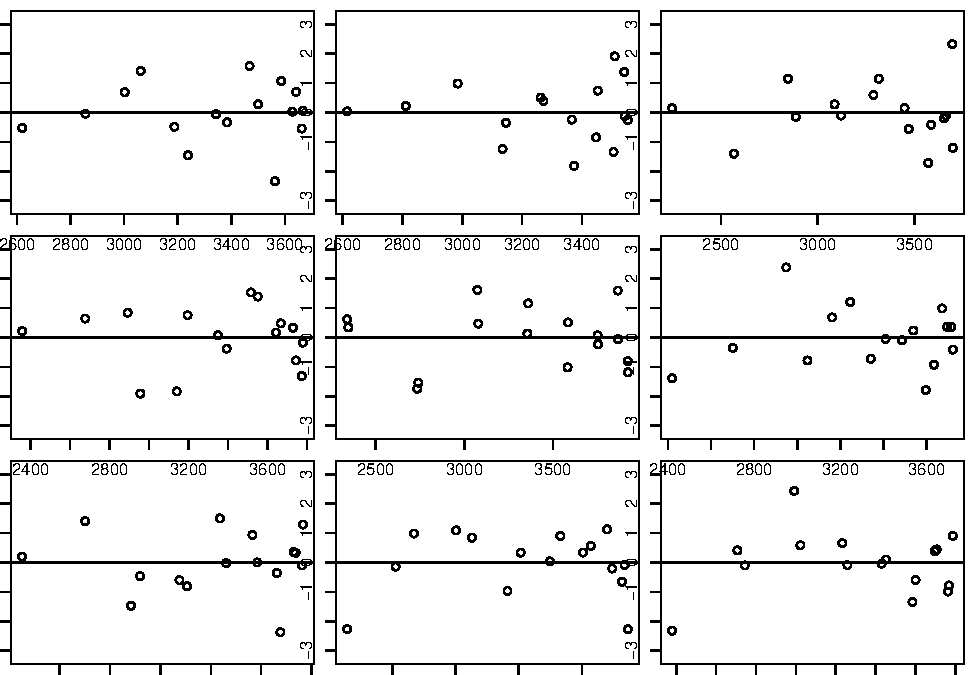
\includegraphics{matstatproblems20-21_files/figure-latex/unnamed-chunk-54-1} \end{center}

Conclusions\ldots.

\hypertarget{section-55}{%
\paragraph{\texorpdfstring{\textbf{6.}}{6.}}\label{section-55}}

The estimates can be obtained with the below code.

\begin{Shaded}
\begin{Highlighting}[]
\KeywordTok{coef}\NormalTok{(kvadreg)}
\end{Highlighting}
\end{Shaded}

\begin{verbatim}
##  (Intercept)         days      daysSqr 
## -1070.397689   293.482948    -4.535802
\end{verbatim}

\begin{Shaded}
\begin{Highlighting}[]
\NormalTok{est <-}\StringTok{ }\KeywordTok{as.numeric}\NormalTok{(}\KeywordTok{coef}\NormalTok{(kvadreg))}
\end{Highlighting}
\end{Shaded}

\begin{verbatim}
## [1] -1070.397689   293.482948    -4.535802
\end{verbatim}

Observe that we are dealing with the model \[
Yield_i=\gamma\cdot daysSqr_i+\beta\cdot days_i+\alpha\equiv\gamma\cdot days_i^2+\beta\cdot days_i+\alpha
\] and as such we know from elementary mathematics that the stationary
point of \(Yield,\,T_{Yield}\equiv\left({optDay,optYield}\right)\) may
be found at \[
T_{Yield}\equiv\left({optDay,optYield}\right)=\left({\frac{-\beta}{2\gamma},\frac{-\left({\beta^2-4\gamma\alpha}\right)}{4\gamma}}\right)
\] As such we may estimate the location of the stationary (toppoint)
point with \[
\hat T_{Yield}\equiv\left({\frac{-\hat\beta}{2\hat\gamma},\frac{-\left({\hat\beta^2-4\hat\gamma\hat\alpha}\right)}{4\hat\gamma}}\right)
\] in 
\includegraphics[width=\textwidth,height=0.16667in]{R_logo.png}
with

\begin{Shaded}
\begin{Highlighting}[]
\NormalTok{optDay <-}\StringTok{ }\OperatorTok{-}\NormalTok{est[}\DecValTok{2}\NormalTok{]}\OperatorTok{/}\NormalTok{(}\DecValTok{2}\OperatorTok{*}\NormalTok{est[}\DecValTok{3}\NormalTok{])}
\end{Highlighting}
\end{Shaded}

\begin{verbatim}
## [1] 32.35183
\end{verbatim}

\begin{Shaded}
\begin{Highlighting}[]
\NormalTok{optYield <-}\StringTok{ }\OperatorTok{-}\StringTok{ }\NormalTok{(est[}\DecValTok{2}\NormalTok{]}\OperatorTok{^}\DecValTok{2} \OperatorTok{-}\StringTok{ }\DecValTok{4}\OperatorTok{*}\NormalTok{est[}\DecValTok{1}\NormalTok{]}\OperatorTok{*}\NormalTok{est[}\DecValTok{3}\NormalTok{]) }\OperatorTok{/}\StringTok{ }\NormalTok{(}\DecValTok{4}\OperatorTok{*}\StringTok{ }\NormalTok{est[}\DecValTok{3}\NormalTok{])}
\end{Highlighting}
\end{Shaded}

\begin{verbatim}
## [1] 3676.957
\end{verbatim}

\hypertarget{section-56}{%
\paragraph{\texorpdfstring{\textbf{7.}}{7.}}\label{section-56}}

The time of harvest \texttt{days} cannot be written as an affine
transformation of our parameters as was the premise in Chapter 9 and 10.
Specifically it will not be possible to find a matrix \(Q\) such that
\(Edays_i=Q\begin{pmatrix}{\alpha\\\beta\\\gamma}\end{pmatrix},\) as
isolation of \texttt{days} in the model would require the use of
squaring and square roots (decidedly non-affine) in accordance with the
quadratic formula.

\hypertarget{section-57}{%
\paragraph{\texorpdfstring{\textbf{8.}}{8.}}\label{section-57}}

We may repeat the tasks of subproblem 6 with the data previously
simulated in \texttt{simYield}

\begin{Shaded}
\begin{Highlighting}[]
\NormalTok{estSim <-}\StringTok{ }\KeywordTok{as.numeric}\NormalTok{(}\KeywordTok{coef}\NormalTok{(kvadreg2))}
\end{Highlighting}
\end{Shaded}

\begin{verbatim}
## [1] -868.700973  279.827547   -4.365983
\end{verbatim}

\begin{Shaded}
\begin{Highlighting}[]
\NormalTok{optDaySim <-}\StringTok{ }\OperatorTok{-}\NormalTok{estSim[}\DecValTok{2}\NormalTok{]}\OperatorTok{/}\NormalTok{(}\DecValTok{2}\OperatorTok{*}\NormalTok{estSim[}\DecValTok{3}\NormalTok{])}
\NormalTok{optYieldSim <-}\StringTok{ }\OperatorTok{-}\StringTok{ }\NormalTok{(estSim[}\DecValTok{2}\NormalTok{]}\OperatorTok{^}\DecValTok{2} \OperatorTok{-}\StringTok{ }\DecValTok{4}\OperatorTok{*}\NormalTok{estSim[}\DecValTok{1}\NormalTok{]}\OperatorTok{*}\NormalTok{estSim[}\DecValTok{3}\NormalTok{]) }\OperatorTok{/}\StringTok{ }\NormalTok{(}\DecValTok{4}\OperatorTok{*}\NormalTok{estSim[}\DecValTok{3}\NormalTok{])}
\KeywordTok{c}\NormalTok{(optDaySim,optYieldSim)}
\end{Highlighting}
\end{Shaded}

\begin{verbatim}
## [1]   32.04634 3615.02303
\end{verbatim}

\hypertarget{section-58}{%
\paragraph{\texorpdfstring{\textbf{9.}}{9.}}\label{section-58}}

We may repeat the above simulation \(1000\) times with

\begin{Shaded}
\begin{Highlighting}[]
\NormalTok{n <-}\StringTok{ }\DecValTok{10}\OperatorTok{^}\DecValTok{3}
\NormalTok{resSim <-}\StringTok{ }\KeywordTok{matrix}\NormalTok{(}\OtherTok{NA}\NormalTok{, n, }\DecValTok{2}\NormalTok{)   }\CommentTok{# Initiation of a matrix}
  \ControlFlowTok{for}\NormalTok{ (i }\ControlFlowTok{in} \DecValTok{1}\OperatorTok{:}\NormalTok{n) \{}
\NormalTok{  simYield <-}\StringTok{ }\KeywordTok{rnorm}\NormalTok{(}\DecValTok{16}\NormalTok{, xi0, sigma0)}
\NormalTok{  kvadregSim <-}\StringTok{ }\KeywordTok{lm}\NormalTok{(simYield }\OperatorTok{~}\StringTok{ }\NormalTok{paddy}\OperatorTok{$}\NormalTok{days }\OperatorTok{+}\StringTok{ }\NormalTok{daysSqr)}
\NormalTok{  estSim <-}\StringTok{ }\KeywordTok{as.numeric}\NormalTok{(}\KeywordTok{coef}\NormalTok{(kvadregSim))}
\NormalTok{  optDaySim <-}\StringTok{ }\OperatorTok{-}\NormalTok{estSim[}\DecValTok{2}\NormalTok{]}\OperatorTok{/}\DecValTok{2}\OperatorTok{/}\NormalTok{estSim[}\DecValTok{3}\NormalTok{]}
\NormalTok{  optYieldSim <-}\StringTok{ }\OperatorTok{-}\StringTok{ }\NormalTok{(estSim[}\DecValTok{2}\NormalTok{]}\OperatorTok{^}\DecValTok{2} \OperatorTok{-}\StringTok{ }\DecValTok{4}\OperatorTok{*}\NormalTok{estSim[}\DecValTok{1}\NormalTok{]}\OperatorTok{*}\NormalTok{estSim[}\DecValTok{3}\NormalTok{]) }\OperatorTok{/}\StringTok{ }\DecValTok{4} \OperatorTok{/}\StringTok{ }\NormalTok{estSim[}\DecValTok{3}\NormalTok{]}
\NormalTok{  resSim[i,}\DecValTok{1}\NormalTok{] <-}\StringTok{ }\NormalTok{optDaySim}
\NormalTok{  resSim[i,}\DecValTok{2}\NormalTok{] <-}\StringTok{ }\NormalTok{optYieldSim}
\NormalTok{\}}
\end{Highlighting}
\end{Shaded}

\hypertarget{section-59}{%
\paragraph{\texorpdfstring{\textbf{10.}}{10.}}\label{section-59}}

We may draw histograms with

\begin{Shaded}
\begin{Highlighting}[]
\KeywordTok{par}\NormalTok{(}\DataTypeTok{mfrow=}\KeywordTok{c}\NormalTok{(}\DecValTok{2}\NormalTok{,}\DecValTok{1}\NormalTok{))}
\KeywordTok{hist}\NormalTok{(resSim[,}\DecValTok{1}\NormalTok{], }\DataTypeTok{main=}\StringTok{"optDay"}\NormalTok{, }\DataTypeTok{breaks =} \DecValTok{30}\NormalTok{)}
\KeywordTok{hist}\NormalTok{(resSim[,}\DecValTok{2}\NormalTok{], }\DataTypeTok{main=}\StringTok{"optYield"}\NormalTok{, }\DataTypeTok{breaks =} \DecValTok{30}\NormalTok{)}
\end{Highlighting}
\end{Shaded}

\begin{center}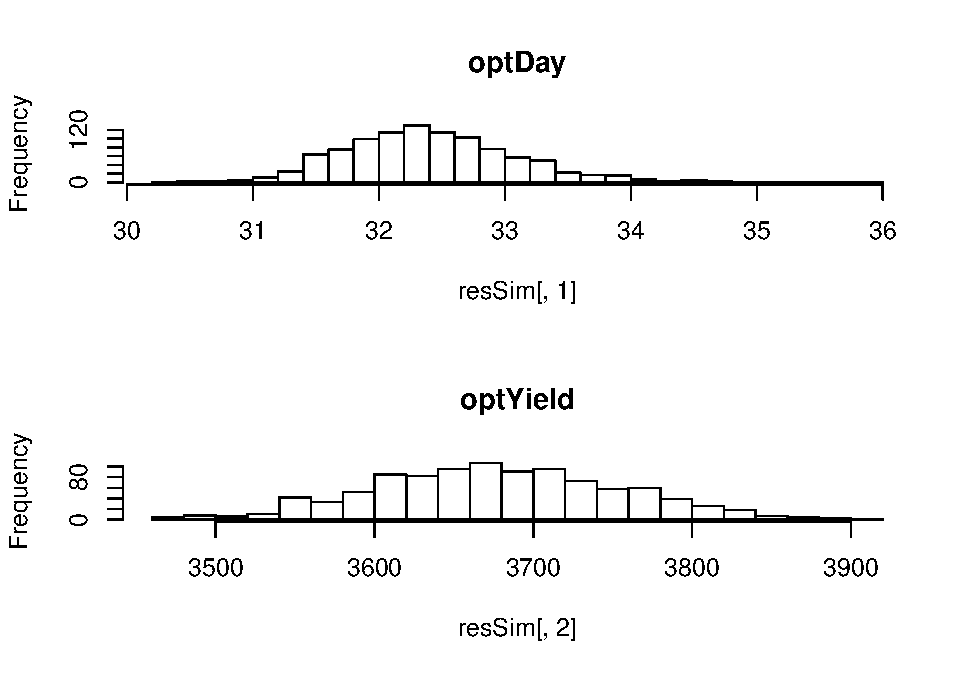
\includegraphics{matstatproblems20-21_files/figure-latex/unnamed-chunk-59-1} \end{center}

It doesn't seem unreasonable to assume that a normal distribution could
fit the data rather well;

\begin{Shaded}
\begin{Highlighting}[]
\NormalTok{fDay <-}\StringTok{ }\ControlFlowTok{function}\NormalTok{(x) }\KeywordTok{dnorm}\NormalTok{(x, }\DataTypeTok{mean =} \KeywordTok{mean}\NormalTok{(resSim[,}\DecValTok{1}\NormalTok{]) , }\DataTypeTok{sd =} \KeywordTok{sd}\NormalTok{(resSim[,}\DecValTok{1}\NormalTok{])) }\CommentTok{#normalfordelingslinien}
\NormalTok{fYield <-}\StringTok{ }\ControlFlowTok{function}\NormalTok{(x) }\KeywordTok{dnorm}\NormalTok{(x,}\DataTypeTok{mean=}\KeywordTok{mean}\NormalTok{(resSim[,}\DecValTok{2}\NormalTok{]), }\DataTypeTok{sd =} \KeywordTok{sd}\NormalTok{(resSim[,}\DecValTok{2}\NormalTok{]))}


\KeywordTok{par}\NormalTok{(}\DataTypeTok{mfrow=}\KeywordTok{c}\NormalTok{(}\DecValTok{2}\NormalTok{,}\DecValTok{1}\NormalTok{))}
\KeywordTok{hist}\NormalTok{(resSim[,}\DecValTok{1}\NormalTok{], }\DataTypeTok{main=}\StringTok{"optDay"}\NormalTok{, }\DataTypeTok{prob=}\NormalTok{T); }\KeywordTok{plot}\NormalTok{(fDay, }\DecValTok{30}\NormalTok{,}\DecValTok{35}\NormalTok{, }\DataTypeTok{add=}\NormalTok{T, }\DataTypeTok{col=}\StringTok{"blue"}\NormalTok{)}
\KeywordTok{hist}\NormalTok{(resSim[,}\DecValTok{2}\NormalTok{], }\DataTypeTok{main=}\StringTok{"optYield"}\NormalTok{, }\DataTypeTok{prob=}\NormalTok{T); }\KeywordTok{plot}\NormalTok{(fYield, }\DecValTok{3400}\NormalTok{,}\DecValTok{3900}\NormalTok{,}\DataTypeTok{add=}\NormalTok{T, }\DataTypeTok{col=}\StringTok{"hot pink"}\NormalTok{)}
\end{Highlighting}
\end{Shaded}

\begin{center}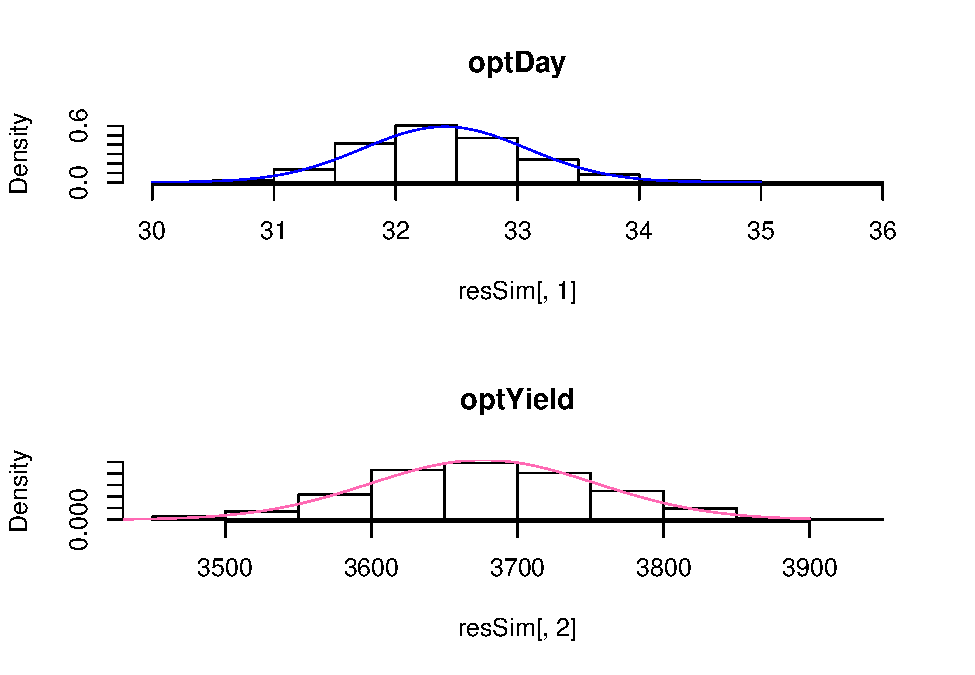
\includegraphics{matstatproblems20-21_files/figure-latex/unnamed-chunk-60-1} \end{center}

\hypertarget{section-60}{%
\paragraph{\texorpdfstring{\textbf{11.}}{11.}}\label{section-60}}

One way to get approximate \(95\%\) confidence intervals for each of
\texttt{optDay,optYield} is to use the quantile function (see
\texttt{?quantile});

\begin{Shaded}
\begin{Highlighting}[]
\KeywordTok{quantile}\NormalTok{((resSim[,}\DecValTok{1}\NormalTok{]),}\KeywordTok{c}\NormalTok{(}\FloatTok{0.025}\NormalTok{,}\FloatTok{0.975}\NormalTok{))}
\end{Highlighting}
\end{Shaded}

\begin{verbatim}
##     2.5%    97.5% 
## 31.27306 33.85067
\end{verbatim}

\begin{Shaded}
\begin{Highlighting}[]
\KeywordTok{quantile}\NormalTok{((resSim[,}\DecValTok{2}\NormalTok{]),}\KeywordTok{c}\NormalTok{(}\FloatTok{0.025}\NormalTok{,}\FloatTok{0.975}\NormalTok{))}
\end{Highlighting}
\end{Shaded}

\begin{verbatim}
##     2.5%    97.5% 
## 3536.514 3827.813
\end{verbatim}

\hypertarget{section-61}{%
\paragraph{\texorpdfstring{\textbf{12.}}{12.}}\label{section-61}}

Based on 16 simulated outcomes, we will be doing a ``linear,
linear-regression'' in order to point out problems with the mean that
arise in this regard, when doing visual model-control with the likes of
residual plots.

\begin{Shaded}
\begin{Highlighting}[]
\NormalTok{simYield <-}\StringTok{ }\KeywordTok{rnorm}\NormalTok{(}\DecValTok{16}\NormalTok{, xi0, sigma0)}
\NormalTok{linRegSim <-}\StringTok{ }\KeywordTok{lm}\NormalTok{(simYield }\OperatorTok{~}\StringTok{ }\NormalTok{paddy}\OperatorTok{$}\NormalTok{days)}
\NormalTok{linresSim <-}\StringTok{ }\KeywordTok{rstandard}\NormalTok{(linRegSim)}
\NormalTok{linfitSim <-}\StringTok{ }\KeywordTok{fitted}\NormalTok{(linRegSim)}
\KeywordTok{plot}\NormalTok{(linfitSim, linresSim, }\DataTypeTok{main =} \StringTok{"(Estimate, Std. Res.)-plot for linear linreg model on simulated data"}\NormalTok{, }\DataTypeTok{xlab =} \StringTok{"Estimated (fitted) Yield"}\NormalTok{, }\DataTypeTok{ylab =}\StringTok{"Standardized residuals"}\NormalTok{, }\DataTypeTok{ylim =} \KeywordTok{c}\NormalTok{(}\OperatorTok{-}\KeywordTok{max}\NormalTok{(}\FloatTok{3.2}\NormalTok{,}\KeywordTok{max}\NormalTok{(}\KeywordTok{abs}\NormalTok{(linresSim))), }\KeywordTok{max}\NormalTok{(}\FloatTok{3.2}\NormalTok{,}\KeywordTok{max}\NormalTok{(}\KeywordTok{abs}\NormalTok{(linresSim)))) );}\KeywordTok{abline}\NormalTok{(}\DecValTok{0}\NormalTok{,}\DecValTok{0}\NormalTok{)}
\end{Highlighting}
\end{Shaded}

\begin{center}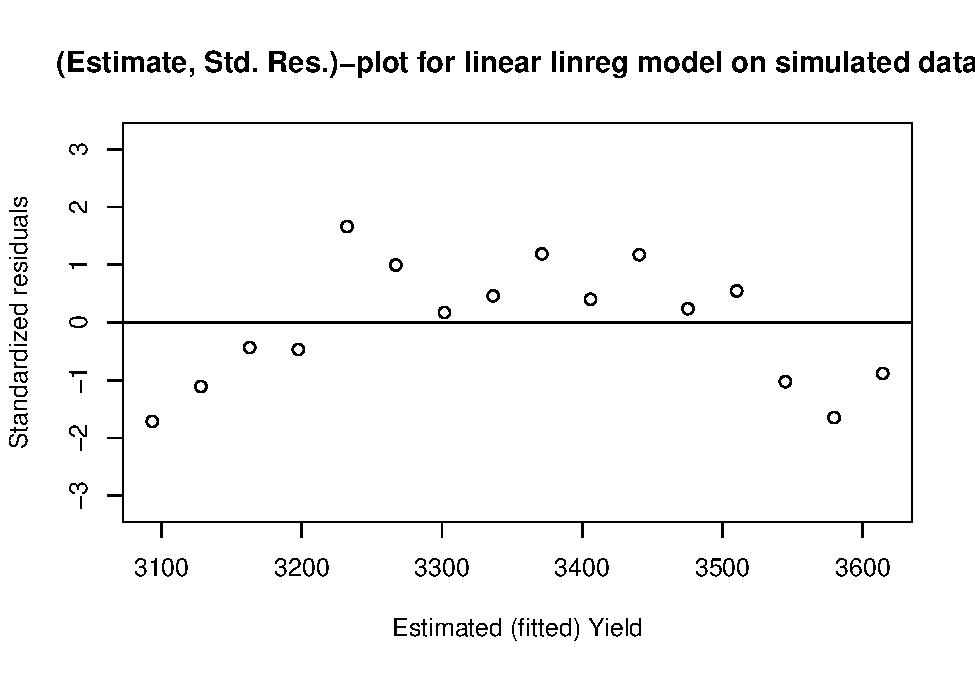
\includegraphics{matstatproblems20-21_files/figure-latex/unnamed-chunk-62-1} \end{center}

Note the clear parabolic shape of the point of the std.-residual plot
above. While the points, as they should, fall within \((-2,2)\) the
manner in which they do so via the aforementioned parabolic shape
suggests that an assumption of the linear relation

\[
EsimYield_i=\zeta+\varphi\cdot days_i
\] is rather implausible.

We may, just as in subproblem 5 repeat the process of simulation;

\begin{Shaded}
\begin{Highlighting}[]
\NormalTok{SimNPlot<-}\ControlFlowTok{function}\NormalTok{(i) \{}
\NormalTok{   simYield <-}\StringTok{ }\KeywordTok{rnorm}\NormalTok{(}\DecValTok{16}\NormalTok{, xi0, sigma0)}
\NormalTok{   linRegSim <-}\StringTok{ }\KeywordTok{lm}\NormalTok{(simYield }\OperatorTok{~}\StringTok{ }\NormalTok{days)}
\NormalTok{   fit <-}\StringTok{ }\KeywordTok{fitted}\NormalTok{(linRegSim)}
\NormalTok{   rst <-}\StringTok{ }\KeywordTok{rstandard}\NormalTok{(linRegSim)}
   \KeywordTok{plot}\NormalTok{(fit, rst, }\DataTypeTok{xlim=}\KeywordTok{c}\NormalTok{(}\DecValTok{3000}\NormalTok{,}\DecValTok{3600}\NormalTok{), }\DataTypeTok{main =} \StringTok{""}\NormalTok{, }\DataTypeTok{xlab =} \StringTok{""}\NormalTok{, }\DataTypeTok{ylab =} \StringTok{""}\NormalTok{, }\DataTypeTok{ylim =} \KeywordTok{c}\NormalTok{(}\OperatorTok{-}\KeywordTok{max}\NormalTok{(}\FloatTok{3.2}\NormalTok{,}\KeywordTok{max}\NormalTok{(}\KeywordTok{abs}\NormalTok{(rst))), }\KeywordTok{max}\NormalTok{(}\FloatTok{3.2}\NormalTok{,}\KeywordTok{max}\NormalTok{(}\KeywordTok{abs}\NormalTok{(rst)))) ) }
   \CommentTok{#Largest symmetric interval (around 0) of (-3.2,3.2) or (-largest absolute rst, largest absolute rst)}
   \KeywordTok{abline}\NormalTok{(}\DecValTok{0}\NormalTok{,}\DecValTok{0}\NormalTok{)}
\NormalTok{\}}

\KeywordTok{par}\NormalTok{(}\DataTypeTok{mfrow =} \KeywordTok{c}\NormalTok{(}\DecValTok{3}\NormalTok{,}\DecValTok{3}\NormalTok{), }\DataTypeTok{mar=}\KeywordTok{c}\NormalTok{(}\FloatTok{0.55}\NormalTok{,}\FloatTok{0.55}\NormalTok{,}\FloatTok{0.55}\NormalTok{,}\FloatTok{0.55}\NormalTok{))}
\ControlFlowTok{for}\NormalTok{ (i }\ControlFlowTok{in} \DecValTok{1}\OperatorTok{:}\DecValTok{9}\NormalTok{) }\KeywordTok{SimNPlot}\NormalTok{(i)}
\end{Highlighting}
\end{Shaded}

\begin{center}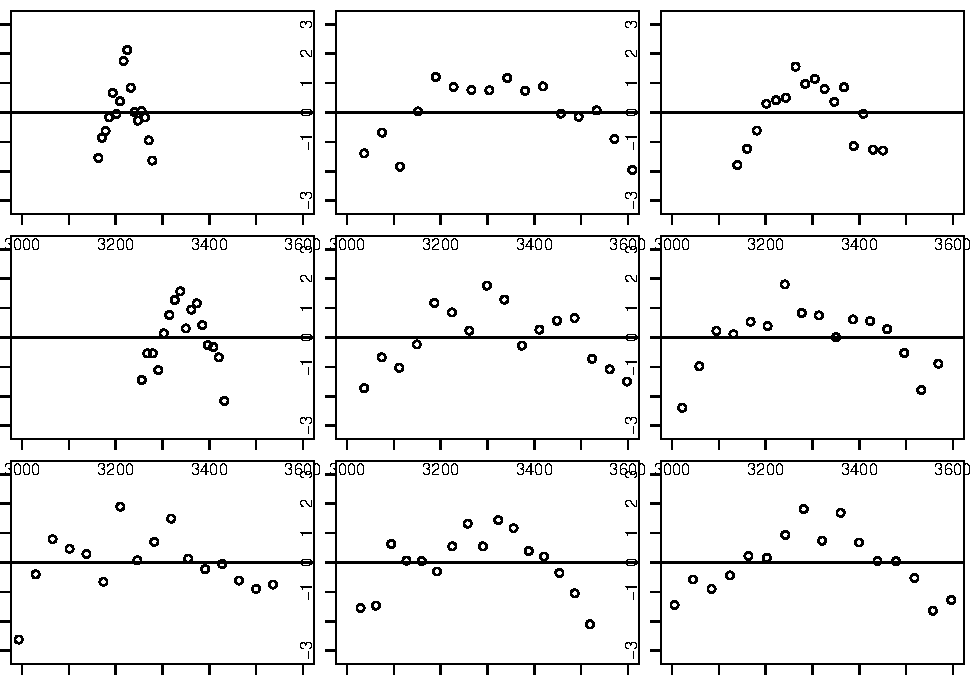
\includegraphics{matstatproblems20-21_files/figure-latex/unnamed-chunk-63-1} \end{center}

Looking at the different simulated plots, notice that a fair bit of
variety appears, though non more so, that we in each case could say that
the linearity assumption is improbable to hold true.

\hypertarget{section-62}{%
\paragraph{\texorpdfstring{\textbf{13.}}{13.}}\label{section-62}}

Below, we will be using the suggested

\includegraphics[width=\textwidth,height=0.16667in]{R_logo.png} commands
to explore the result of fudging with the variance when doing std.
residual plots. Note that one may examine \texttt{?points} for further
details regarding this command.

\begin{Shaded}
\begin{Highlighting}[]
\NormalTok{newSD <-}\StringTok{ }\DecValTok{25}\OperatorTok{*}\NormalTok{(}\DecValTok{15}\OperatorTok{-}\KeywordTok{abs}\NormalTok{(paddy}\OperatorTok{$}\NormalTok{days}\DecValTok{-31}\NormalTok{))}
\NormalTok{newSD}
\end{Highlighting}
\end{Shaded}

\begin{verbatim}
##  [1]   0  50 100 150 200 250 300 350 350 300 250 200 150 100  50   0
\end{verbatim}

\begin{Shaded}
\begin{Highlighting}[]
\NormalTok{simYield <-}\StringTok{ }\KeywordTok{rnorm}\NormalTok{(}\DecValTok{16}\NormalTok{, xi0, newSD)}
\KeywordTok{plot}\NormalTok{(paddy}\OperatorTok{$}\NormalTok{days, simYield)}
\KeywordTok{points}\NormalTok{(paddy}\OperatorTok{$}\NormalTok{days, xi0, }\DataTypeTok{type=}\StringTok{"l"}\NormalTok{)}
\end{Highlighting}
\end{Shaded}

\begin{center}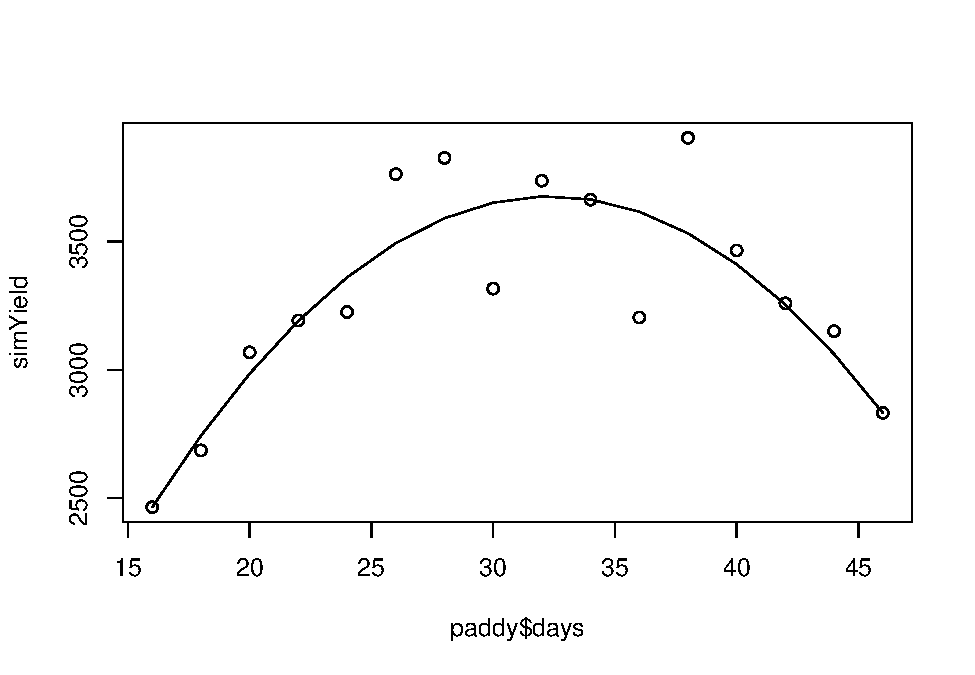
\includegraphics{matstatproblems20-21_files/figure-latex/unnamed-chunk-64-1} \end{center}

Above, we are manipulating the standard deviation, as shown when calling
\texttt{newSD}, that assigns a symmetrically high deviation to the
``middle simulations'' of the simulated \(16\)-datapoints - ie. we
assign the highest deviation to the \(8,9\)th draw from the normal
distribution, and then progressively and symmetrically lower deviation
towards the ``edges''.

The result of the above procedure when plotting \texttt{simYield}
against \texttt{days} is that as \texttt{days} are ordered, the i'th
\texttt{Yield}-simulation (the middle of which have now been simulated
with greater variance) will be assumed to be connected with the
corresponding i'th day.

Consequently for the ``quadratic'' standardized-residual plot

\begin{Shaded}
\begin{Highlighting}[]
\NormalTok{kvadregSim <-}\StringTok{ }\KeywordTok{lm}\NormalTok{(simYield }\OperatorTok{~}\StringTok{ }\NormalTok{paddy}\OperatorTok{$}\NormalTok{days }\OperatorTok{+}\StringTok{ }\NormalTok{daysSqr)}
\NormalTok{resSim <-}\StringTok{ }\KeywordTok{rstandard}\NormalTok{(kvadregSim)}
\NormalTok{fitSim <-}\StringTok{ }\KeywordTok{fitted}\NormalTok{(kvadregSim)}
\KeywordTok{plot}\NormalTok{(fitSim, resSim, }\DataTypeTok{main =} \StringTok{"(Estimate, Std. Res.)-plot"}\NormalTok{, }\DataTypeTok{xlab =} \StringTok{"Estimated (fitted) Yield"}\NormalTok{, }\DataTypeTok{ylab =}\StringTok{"Standardized residuals"}\NormalTok{, }\DataTypeTok{ylim =} \KeywordTok{c}\NormalTok{(}\OperatorTok{-}\KeywordTok{max}\NormalTok{(}\FloatTok{3.2}\NormalTok{,}\KeywordTok{max}\NormalTok{(}\KeywordTok{abs}\NormalTok{(linresSim))), }\KeywordTok{max}\NormalTok{(}\FloatTok{3.2}\NormalTok{,}\KeywordTok{max}\NormalTok{(}\KeywordTok{abs}\NormalTok{(linresSim)))) );}\KeywordTok{abline}\NormalTok{(}\DataTypeTok{h=}\DecValTok{0}\NormalTok{,}\DataTypeTok{lty=}\DecValTok{2}\NormalTok{)}
\end{Highlighting}
\end{Shaded}

\begin{center}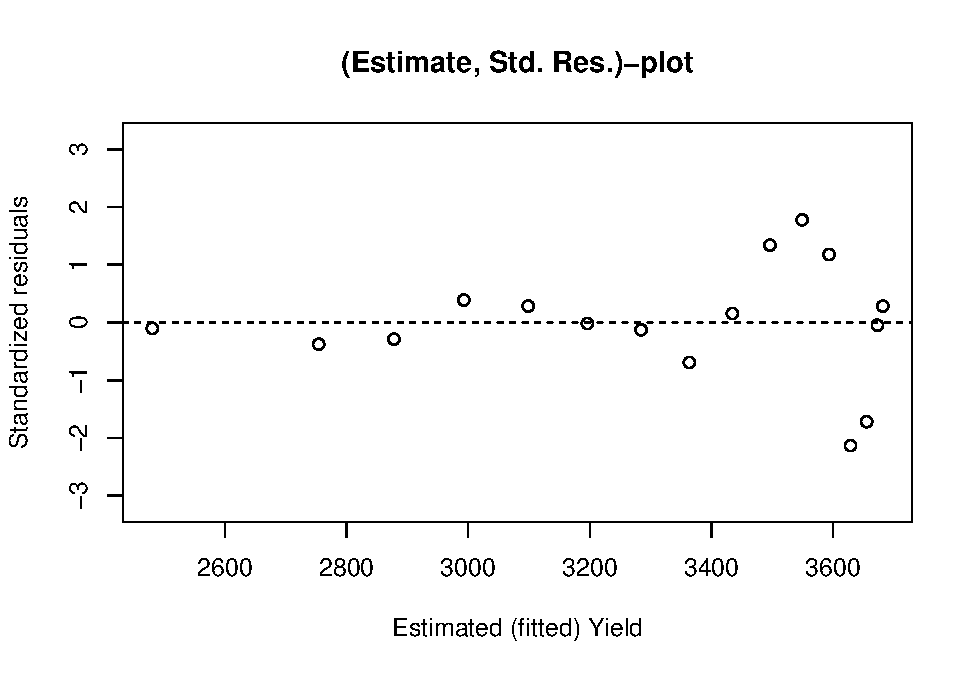
\includegraphics{matstatproblems20-21_files/figure-latex/unnamed-chunk-65-1} \end{center}

Note that the highest fitted \texttt{Yield} values seem to be
significantly more spread out than the rest.

We may simulate more datasets to explore the reproducibility of this
result

\begin{Shaded}
\begin{Highlighting}[]
\KeywordTok{par}\NormalTok{(}\DataTypeTok{mfrow =} \KeywordTok{c}\NormalTok{(}\DecValTok{3}\NormalTok{,}\DecValTok{3}\NormalTok{), }\DataTypeTok{mar=}\KeywordTok{c}\NormalTok{(}\FloatTok{0.55}\NormalTok{,}\FloatTok{0.55}\NormalTok{,}\FloatTok{0.55}\NormalTok{,}\FloatTok{0.55}\NormalTok{))}
\ControlFlowTok{for}\NormalTok{ (i }\ControlFlowTok{in} \DecValTok{1}\OperatorTok{:}\DecValTok{9}\NormalTok{)\{}
\NormalTok{  simYield <-}\StringTok{ }\KeywordTok{rnorm}\NormalTok{(}\DecValTok{16}\NormalTok{, xi0, newSD)}
\NormalTok{  kvadregSim <-}\StringTok{ }\KeywordTok{lm}\NormalTok{(simYield }\OperatorTok{~}\StringTok{ }\NormalTok{paddy}\OperatorTok{$}\NormalTok{days }\OperatorTok{+}\StringTok{ }\NormalTok{daysSqr)}
\NormalTok{  resSim <-}\StringTok{ }\KeywordTok{rstandard}\NormalTok{(kvadregSim)}
\NormalTok{  fitSim <-}\StringTok{ }\KeywordTok{fitted}\NormalTok{(kvadregSim)}
  \KeywordTok{plot}\NormalTok{(fitSim,resSim, }\DataTypeTok{xlim=}\KeywordTok{c}\NormalTok{(}\DecValTok{2400}\NormalTok{,}\DecValTok{4000}\NormalTok{), }\DataTypeTok{main =} \StringTok{""}\NormalTok{, }\DataTypeTok{xlab =} \StringTok{""}\NormalTok{, }\DataTypeTok{ylab =} \StringTok{""}\NormalTok{, }\DataTypeTok{ylim =} \KeywordTok{c}\NormalTok{(}\OperatorTok{-}\KeywordTok{max}\NormalTok{(}\FloatTok{3.2}\NormalTok{,}\KeywordTok{max}\NormalTok{(}\KeywordTok{abs}\NormalTok{(rst))), }\KeywordTok{max}\NormalTok{(}\FloatTok{3.2}\NormalTok{,}\KeywordTok{max}\NormalTok{(}\KeywordTok{abs}\NormalTok{(rst))))) ;}\KeywordTok{abline}\NormalTok{(}\DataTypeTok{h=}\DecValTok{0}\NormalTok{,}\DataTypeTok{lty=}\DecValTok{2}\NormalTok{)}
\NormalTok{\}}
\end{Highlighting}
\end{Shaded}

\begin{center}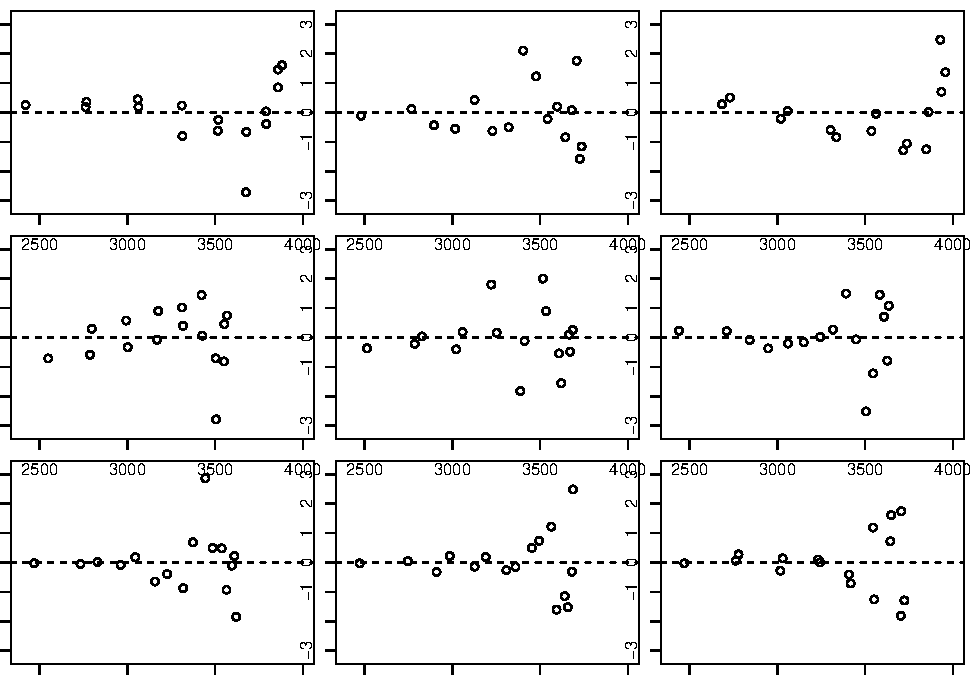
\includegraphics{matstatproblems20-21_files/figure-latex/unnamed-chunk-66-1} \end{center}

The simulated datasets seem rather ``trumpet shaped'' as in it seems
that the standard residuals posses an increased variance toward the
higher \texttt{Yield} values. - This is in accordance with the procedure
by which data was simulated, as we have simulated larger standard
deviation for the middle datapoints, which, in accordance with the
quadratic linear regression model, also tend to have larger value - ie.
we would expect to see larger variance for the larger values of the
dataset. This in return will then transfer onto the residuals, which we,
in keeping with plots above, are expected to be more spread out, towards
the larger \texttt{Yield} values.

\hypertarget{hs-14}{%
\subsection{HS 14}\label{hs-14}}

\hypertarget{section-63}{%
\paragraph{\texorpdfstring{\textbf{1.}}{1.}}\label{section-63}}

If one were primarily to be interested in predicting fat percentages
through ``the use of the other variables'', one might try a linear
regression model of the form;

\emph{For \(Fat_1,\ldots Fat_N\) independent normally distributed with
variance homogeneity of \(\sigma^2\) and mean
\(EFat_i=\alpha+\beta\cdot Triceps_i+\gamma\cdot Thigh_i+\delta\cdot Midarm_i,\,\,i=1,\ldots,N.\)}

\hypertarget{section-64}{%
\paragraph{\texorpdfstring{\textbf{2.}}{2.}}\label{section-64}}

We may start off with importing the relevant dataset;

\begin{Shaded}
\begin{Highlighting}[]
\NormalTok{bodyfat <-}\StringTok{ }\KeywordTok{read_table2}\NormalTok{(}\StringTok{"bodyfat.txt"}\NormalTok{)}
\end{Highlighting}
\end{Shaded}

\begin{verbatim}
## Parsed with column specification:
## cols(
##   Fat = col_double(),
##   Triceps = col_double(),
##   Thigh = col_double(),
##   Midarm = col_double()
## )
\end{verbatim}

\begin{Shaded}
\begin{Highlighting}[]
\KeywordTok{head}\NormalTok{(bodyfat)}
\end{Highlighting}
\end{Shaded}

\begin{verbatim}
## # A tibble: 6 x 4
##     Fat Triceps Thigh Midarm
##   <dbl>   <dbl> <dbl>  <dbl>
## 1  11.9    19.5  43.1   29.1
## 2  22.8    24.7  49.8   28.2
## 3  18.7    30.7  51.9   37  
## 4  20.1    29.8  54.3   31.1
## 5  12.9    19.1  42.2   30.9
## 6  21.7    25.6  53.9   23.7
\end{verbatim}

as well as using the commands

\begin{Shaded}
\begin{Highlighting}[]
\KeywordTok{plot}\NormalTok{(bodyfat)}
\end{Highlighting}
\end{Shaded}

\begin{center}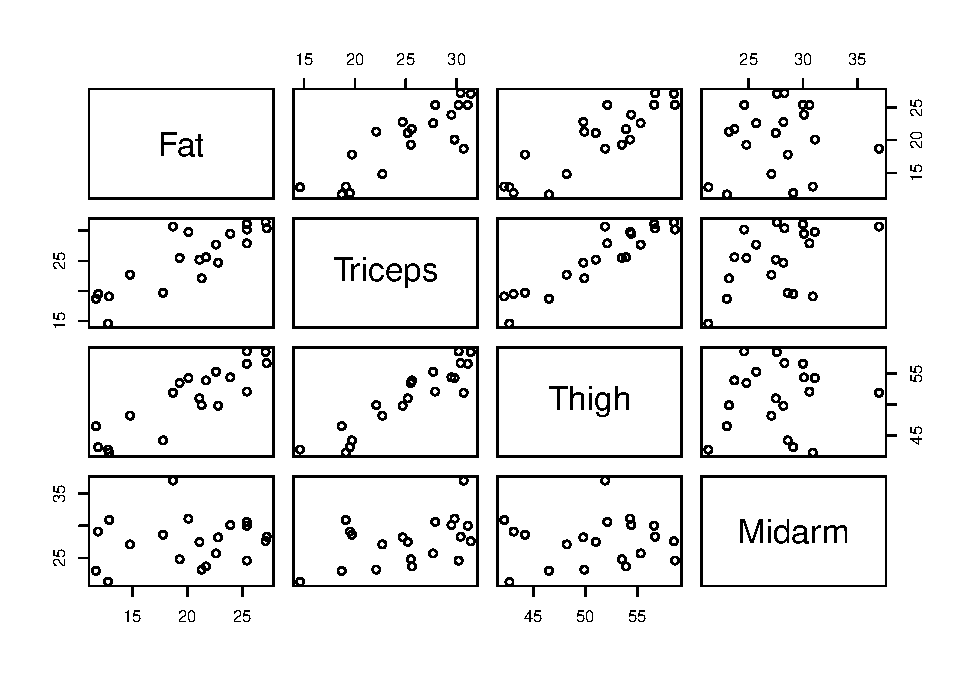
\includegraphics{matstatproblems20-21_files/figure-latex/unnamed-chunk-68-1} \end{center}

\begin{Shaded}
\begin{Highlighting}[]
\KeywordTok{cor}\NormalTok{(bodyfat)}
\end{Highlighting}
\end{Shaded}

\begin{verbatim}
##               Fat   Triceps     Thigh    Midarm
## Fat     1.0000000 0.8432654 0.8780896 0.1424440
## Triceps 0.8432654 1.0000000 0.9238425 0.4577772
## Thigh   0.8780896 0.9238425 1.0000000 0.0846675
## Midarm  0.1424440 0.4577772 0.0846675 1.0000000
\end{verbatim}

Looking at \texttt{?cor} one might conclude that cor generates a
correlation matrix for the dataset. The ``wierd'' appearance of the
above plot is caused by the fact that we have a total of four variables
at play in the dataset, such that there are \(4\cdot 4 = 16\) different
ways of plotting one plot against another. Of the \(16\) however, four
include plotting of the variables against themself, which is rather
silly, and thus the resulting plot is created by

\includegraphics[width=\textwidth,height=0.16667in]{R_logo.png}.

\hypertarget{section-65}{%
\paragraph{\texorpdfstring{\textbf{3.}}{3.}}\label{section-65}}

We will be fitting the model from subproblem 1 using \texttt{lm}

\begin{Shaded}
\begin{Highlighting}[]
\NormalTok{m1 <-}\StringTok{ }\KeywordTok{lm}\NormalTok{(Fat }\OperatorTok{~}\StringTok{ }\NormalTok{Triceps }\OperatorTok{+}\StringTok{ }\NormalTok{Thigh }\OperatorTok{+}\StringTok{ }\NormalTok{Midarm, }\DataTypeTok{data =}\NormalTok{ bodyfat)}
\end{Highlighting}
\end{Shaded}

We might also do a visual modelcontrol through the use of a standardized
residual plot;

\begin{Shaded}
\begin{Highlighting}[]
\NormalTok{rst <-}\StringTok{ }\KeywordTok{rstandard}\NormalTok{(m1)}
\NormalTok{fit <-}\StringTok{ }\KeywordTok{fitted}\NormalTok{(m1)}
\KeywordTok{plot}\NormalTok{(fit, rst, }\DataTypeTok{main =} \StringTok{"(Estimate, Std. Res.)-plot"}\NormalTok{, }\DataTypeTok{xlab =} \StringTok{"Estimated (fitted) Fat Percentage"}\NormalTok{, }\DataTypeTok{ylab =}\StringTok{"Standardized residuals"}\NormalTok{, }\DataTypeTok{ylim =} \KeywordTok{c}\NormalTok{(}\OperatorTok{-}\KeywordTok{max}\NormalTok{(}\FloatTok{3.2}\NormalTok{,}\KeywordTok{max}\NormalTok{(}\KeywordTok{abs}\NormalTok{(rst))), }\KeywordTok{max}\NormalTok{(}\FloatTok{3.2}\NormalTok{,}\KeywordTok{max}\NormalTok{(}\KeywordTok{abs}\NormalTok{(rst)))) );}\KeywordTok{abline}\NormalTok{(}\DataTypeTok{h=}\DecValTok{0}\NormalTok{,}\DataTypeTok{lty=}\DecValTok{2}\NormalTok{)}
\end{Highlighting}
\end{Shaded}

\begin{center}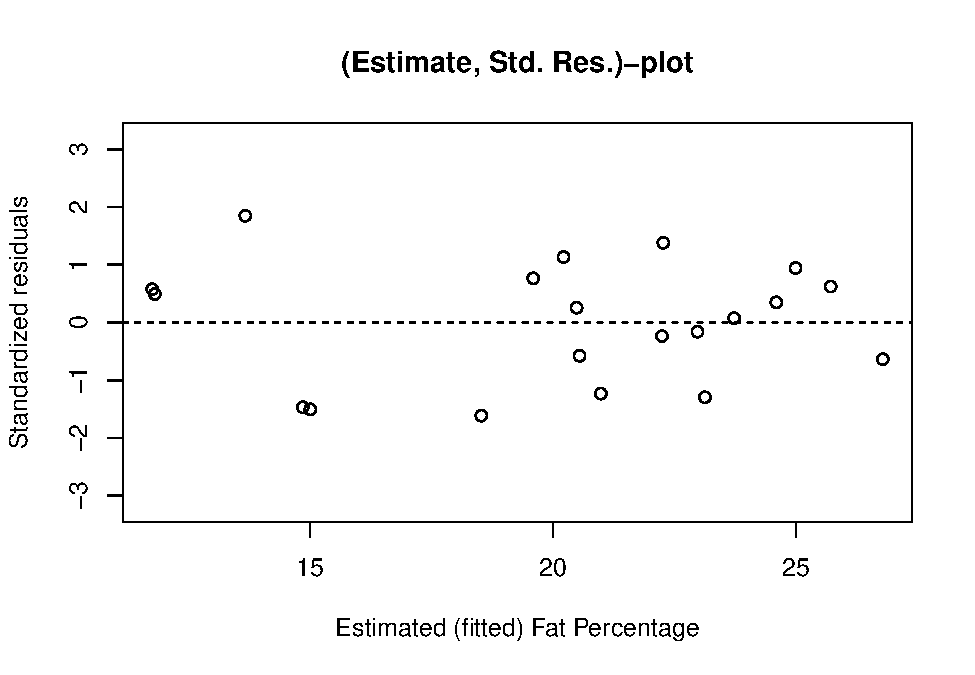
\includegraphics{matstatproblems20-21_files/figure-latex/unnamed-chunk-70-1} \end{center}

Which looks rather respectable on all fronts.

\hypertarget{section-66}{%
\paragraph{\texorpdfstring{\textbf{4.}}{4.}}\label{section-66}}

We may look at the \texttt{summary(m1)} object;

\begin{Shaded}
\begin{Highlighting}[]
\KeywordTok{summary}\NormalTok{(m1)}
\end{Highlighting}
\end{Shaded}

\begin{verbatim}
## 
## Call:
## lm(formula = Fat ~ Triceps + Thigh + Midarm, data = bodyfat)
## 
## Residuals:
##     Min      1Q  Median      3Q     Max 
## -3.7263 -1.6111  0.3923  1.4656  4.1277 
## 
## Coefficients:
##             Estimate Std. Error t value Pr(>|t|)
## (Intercept)  117.085     99.782   1.173    0.258
## Triceps        4.334      3.016   1.437    0.170
## Thigh         -2.857      2.582  -1.106    0.285
## Midarm        -2.186      1.595  -1.370    0.190
## 
## Residual standard error: 2.48 on 16 degrees of freedom
## Multiple R-squared:  0.8014, Adjusted R-squared:  0.7641 
## F-statistic: 21.52 on 3 and 16 DF,  p-value: 7.343e-06
\end{verbatim}

Amongst the coefficient parameters we find the \texttt{t-static} values.
There are of the form \[
t_{\hat\zeta}=\frac{\hat\zeta-\zeta_0}{se(\hat\zeta)},
\] for some corresponding parameter \(\zeta\) of our model. By default

\includegraphics[width=\textwidth,height=0.16667in]{R_logo.png} sets
\(\zeta_0=0,\) leaving the \texttt{t\ values} that appear, resulting
from division of the estimate for the parameter with its standard error,
ie with \(\zeta_0=0\) be have
\(t_{\hat\zeta}=\frac{\hat\zeta}{se(\hat\zeta)}.\)

With these \texttt{t\ values} the corresponding
\texttt{Pr(\textgreater{}\textbar{}t\textbar{})}-values are the
symmetric tail probabilities (p values) of getting t values of greater
magnitude than \(t_{\hat\zeta}\) in a student t - distribution with
\texttt{m1\$df.residual=16} degrees of freedom, ie. p values:
probability of obtaining test results at least as extreme as the results
actually observed, under the assumption that the null hypothesis is
correct, such that small values are critical to the hypothesis. We may
formalize the writing of the p-values; For \(T\sim t_{16}\), the to
\(\zeta\) corresponding \texttt{Pr(\textgreater{}\textbar{}t\textbar{})}
value, is \[
P(|T|>|t|)\overset{\text{symmetry}}{=}2P(T>|t|).
\] As an example of a manual calculation of one of the p-values being
carried out, we could approach the hypothesis; \[
H:\,\alpha = 0
\] which by the model corresponds to the hypothesis that the intercept
is \(0.\)

\begin{Shaded}
\begin{Highlighting}[]
\NormalTok{(degfree <-}\StringTok{ }\NormalTok{m1}\OperatorTok{$}\NormalTok{df.residual)}
\end{Highlighting}
\end{Shaded}

\begin{verbatim}
## [1] 16
\end{verbatim}

\begin{Shaded}
\begin{Highlighting}[]
\NormalTok{hatalpha <-}\StringTok{ }\KeywordTok{coef}\NormalTok{(}\KeywordTok{summary}\NormalTok{(m1))[}\DecValTok{1}\NormalTok{,}\DecValTok{1}\NormalTok{]}
\end{Highlighting}
\end{Shaded}

\begin{verbatim}
## [1] 117.0847
\end{verbatim}

\begin{Shaded}
\begin{Highlighting}[]
\NormalTok{sealpha <-}\StringTok{ }\KeywordTok{coef}\NormalTok{(}\KeywordTok{summary}\NormalTok{(m1))[}\DecValTok{1}\NormalTok{,}\DecValTok{2}\NormalTok{]}
\end{Highlighting}
\end{Shaded}

\begin{verbatim}
## [1] 99.7824
\end{verbatim}

\begin{Shaded}
\begin{Highlighting}[]
\NormalTok{t_alpha <-}\StringTok{ }\KeywordTok{coef}\NormalTok{(}\KeywordTok{summary}\NormalTok{(m1))[}\DecValTok{1}\NormalTok{,}\DecValTok{3}\NormalTok{]}
\end{Highlighting}
\end{Shaded}

\begin{verbatim}
## [1] 1.1734
\end{verbatim}

\begin{Shaded}
\begin{Highlighting}[]
\NormalTok{pt_alpha <-}\StringTok{ }\DecValTok{2}\OperatorTok{*}\KeywordTok{pt}\NormalTok{(t_alpha, degfree, }\DataTypeTok{lower.tail =}\NormalTok{ F)}
\end{Highlighting}
\end{Shaded}

\begin{verbatim}
## [1] 0.2578078
\end{verbatim}

\begin{Shaded}
\begin{Highlighting}[]
\NormalTok{pt_alpha}\OperatorTok{-}\KeywordTok{coef}\NormalTok{(}\KeywordTok{summary}\NormalTok{(m1))[}\DecValTok{1}\NormalTok{,}\DecValTok{4}\NormalTok{] }\CommentTok{#Is there a difference between our p-value, and summary's? <- nope.}
\end{Highlighting}
\end{Shaded}

\begin{verbatim}
## [1] 0
\end{verbatim}

Looking at the p-value vector

\begin{Shaded}
\begin{Highlighting}[]
\NormalTok{pvalvec <-}\StringTok{ }\KeywordTok{coef}\NormalTok{(}\KeywordTok{summary}\NormalTok{(m1))[,}\DecValTok{4}\NormalTok{]}
\NormalTok{pvalvec}
\end{Highlighting}
\end{Shaded}

\begin{verbatim}
## (Intercept)     Triceps       Thigh      Midarm 
##   0.2578078   0.1699111   0.2848944   0.1895628
\end{verbatim}

we might conclude that while there is not a lot of support for the
various ``marginal'' null hypotheses, the p values are at the same time
not so critical (small) that we may immediately dismiss any of the null
hypotheses.

\hypertarget{section-67}{%
\paragraph{\texorpdfstring{\textbf{5.}}{5.}}\label{section-67}}

After looking through \texttt{?anova}, we may use the recommended
commands

\begin{Shaded}
\begin{Highlighting}[]
\NormalTok{m2 <-}\StringTok{ }\KeywordTok{lm}\NormalTok{(Fat }\OperatorTok{~}\StringTok{ }\NormalTok{Midarm, }\DataTypeTok{data =}\NormalTok{ bodyfat)}
\KeywordTok{anova}\NormalTok{(m2,m1)}
\end{Highlighting}
\end{Shaded}

\begin{verbatim}
## Analysis of Variance Table
## 
## Model 1: Fat ~ Midarm
## Model 2: Fat ~ Triceps + Thigh + Midarm
##   Res.Df    RSS Df Sum of Sq      F    Pr(>F)    
## 1     18 485.34                                  
## 2     16  98.40  2    386.93 31.456 2.856e-06 ***
## ---
## Signif. codes:  0 '***' 0.001 '**' 0.01 '*' 0.05 '.' 0.1 ' ' 1
\end{verbatim}

\textbf{\emph{Conclusion\ldots{}}}

\hypertarget{section-68}{%
\paragraph{\texorpdfstring{\textbf{6.}}{6.}}\label{section-68}}

\hypertarget{section-69}{%
\paragraph{\texorpdfstring{\textbf{7.}}{7.}}\label{section-69}}

\hypertarget{section-70}{%
\paragraph{\texorpdfstring{\textbf{8.}}{8.}}\label{section-70}}

\hypertarget{section-71}{%
\paragraph{\texorpdfstring{\textbf{9.}}{9.}}\label{section-71}}

\hypertarget{hs-15}{%
\subsection{HS 15}\label{hs-15}}

We may import the dataset;

\begin{Shaded}
\begin{Highlighting}[]
\NormalTok{engel <-}\StringTok{ }\KeywordTok{read_table2}\NormalTok{(}\StringTok{"engel.txt"}\NormalTok{) }\CommentTok{#read_table2 = whitespace delimiter}
\end{Highlighting}
\end{Shaded}

\begin{verbatim}
## Parsed with column specification:
## cols(
##   income = col_double(),
##   foodexp = col_double()
## )
\end{verbatim}

\hypertarget{section-72}{%
\paragraph{\texorpdfstring{\textbf{1.}}{1.}}\label{section-72}}

Having registered both the income and the amount spent on food for
different households, one might imagine that the amount spent on food
could within some sort of causal structure be seen as a function of the
income of the corresponding household. We may hold the hypothesis that a
household with more income might translate to a household with more
disposable income, and that a household with more disposable income
would then dispence more of this towards food. We might create the
corresponding scatterplot

\begin{Shaded}
\begin{Highlighting}[]
\NormalTok{foodexp <-}\StringTok{ }\NormalTok{engel}\OperatorTok{$}\NormalTok{foodexp }\CommentTok{#Note that 'attach' only has scope of the current R-chunck}
\NormalTok{income <-}\StringTok{ }\NormalTok{engel}\OperatorTok{$}\NormalTok{income }\CommentTok{#Note that 'attach' only has scope of the current R-chunck}
\NormalTok{p <-}\StringTok{ }\KeywordTok{ggplot}\NormalTok{(}\DataTypeTok{data =}\NormalTok{ engel)}
\NormalTok{p_}\DecValTok{1}\NormalTok{ <-}\StringTok{ }\KeywordTok{geom_point}\NormalTok{(}\DataTypeTok{mapping =} \KeywordTok{aes}\NormalTok{(}\DataTypeTok{x=}\NormalTok{income, }\DataTypeTok{y =}\NormalTok{ foodexp))}
\NormalTok{p}\OperatorTok{+}\NormalTok{p_}\DecValTok{1}
\end{Highlighting}
\end{Shaded}

\begin{center}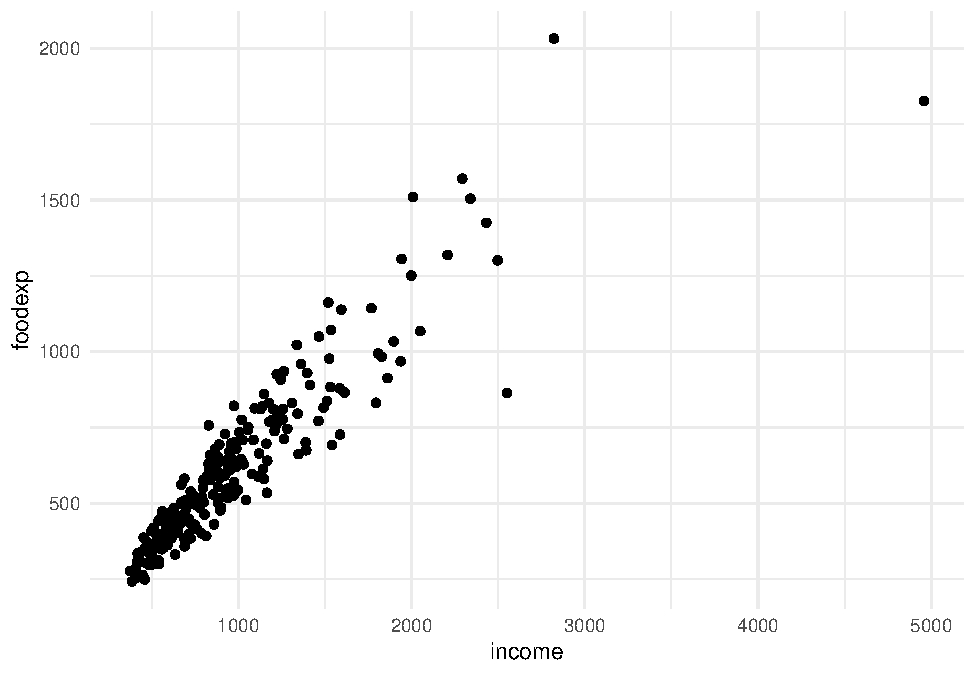
\includegraphics{matstatproblems20-21_files/figure-latex/unnamed-chunk-76-1} \end{center}

It seem like there is a central body of observations that could have
some sort of underlying linear trend going on, though it appears as if
the observations are more spread out the higher the income within the
central body. There also seem to be three outliers from this central
body of observations, that are probably going to have a fair bit of sway
in deriving a linear fit.

\hypertarget{section-73}{%
\paragraph{\texorpdfstring{\textbf{2.}}{2.}}\label{section-73}}

By subproblem 1 it doesn't seem totally unreasonable to write the
statistical model;

\emph{Let \(foodexp_1,\ldots foodexp_{235}\) independent normally
distributed with variance homogeneity of \(\sigma^2\) and mean
\(Efoodexp_i=\alpha+\beta\cdot Income_i+\epsilon_i,\,\,\epsilon_i\sim\mathcal{N}\left({{0},{\sigma^2}}\right)\,\,i=1,\ldots,235.\)}

We may fit this model in

\includegraphics[width=\textwidth,height=0.16667in]{R_logo.png} with

\begin{Shaded}
\begin{Highlighting}[]
\NormalTok{model <-}\StringTok{ }\KeywordTok{lm}\NormalTok{(foodexp }\OperatorTok{~}\StringTok{ }\NormalTok{income, }\DataTypeTok{data =}\NormalTok{ engel)}
\end{Highlighting}
\end{Shaded}

We might then do a visual model control through a standardized residual
plot, and a QQ-plot;

\begin{Shaded}
\begin{Highlighting}[]
\NormalTok{fit <-}\StringTok{ }\KeywordTok{fitted}\NormalTok{(model)}
\NormalTok{rst <-}\StringTok{ }\KeywordTok{rstandard}\NormalTok{(model)}
\KeywordTok{library}\NormalTok{(gridExtra)}
\end{Highlighting}
\end{Shaded}

\begin{verbatim}
## 
## Attaching package: 'gridExtra'
\end{verbatim}

\begin{verbatim}
## The following object is masked from 'package:dplyr':
## 
##     combine
\end{verbatim}

\begin{Shaded}
\begin{Highlighting}[]
\NormalTok{p_}\DecValTok{2}\NormalTok{ <-}\StringTok{ }\KeywordTok{qplot}\NormalTok{(fit, rst, }\DataTypeTok{main =} \StringTok{"(Estimate, Std. Res.)-plot for linreg model on engel"}\NormalTok{, }\DataTypeTok{xlab =} \StringTok{"Estimated (fitted) foodexpence"}\NormalTok{, }\DataTypeTok{ylab =}\StringTok{"Standardized residuals"}\NormalTok{, }\DataTypeTok{ylim =} \KeywordTok{c}\NormalTok{(}\OperatorTok{-}\KeywordTok{max}\NormalTok{(}\FloatTok{3.2}\NormalTok{,}\KeywordTok{max}\NormalTok{(}\KeywordTok{abs}\NormalTok{(rst))), }\KeywordTok{max}\NormalTok{(}\FloatTok{3.2}\NormalTok{,}\KeywordTok{max}\NormalTok{(}\KeywordTok{abs}\NormalTok{(rst)))) )}\OperatorTok{+}\KeywordTok{geom_hline}\NormalTok{(}\DataTypeTok{yintercept =} \DecValTok{0}\NormalTok{) }\CommentTok{#Largest symmetric interval (around 0) of (-3.2,3.2) or (-largest absolute rst, largest absolute rst)}
\NormalTok{p_}\DecValTok{3}\NormalTok{ <-}\StringTok{ }\NormalTok{p }\OperatorTok{+}\StringTok{ }\KeywordTok{geom_qq}\NormalTok{() }\OperatorTok{+}\StringTok{ }\KeywordTok{geom_qq_line}\NormalTok{() }\OperatorTok{+}\StringTok{ }\KeywordTok{aes}\NormalTok{(}\DataTypeTok{sample =}\NormalTok{ rst)}
\KeywordTok{grid.arrange}\NormalTok{(p_}\DecValTok{2}\NormalTok{,p_}\DecValTok{3}\NormalTok{, }\DataTypeTok{ncol =} \DecValTok{2}\NormalTok{)}
\end{Highlighting}
\end{Shaded}

\begin{center}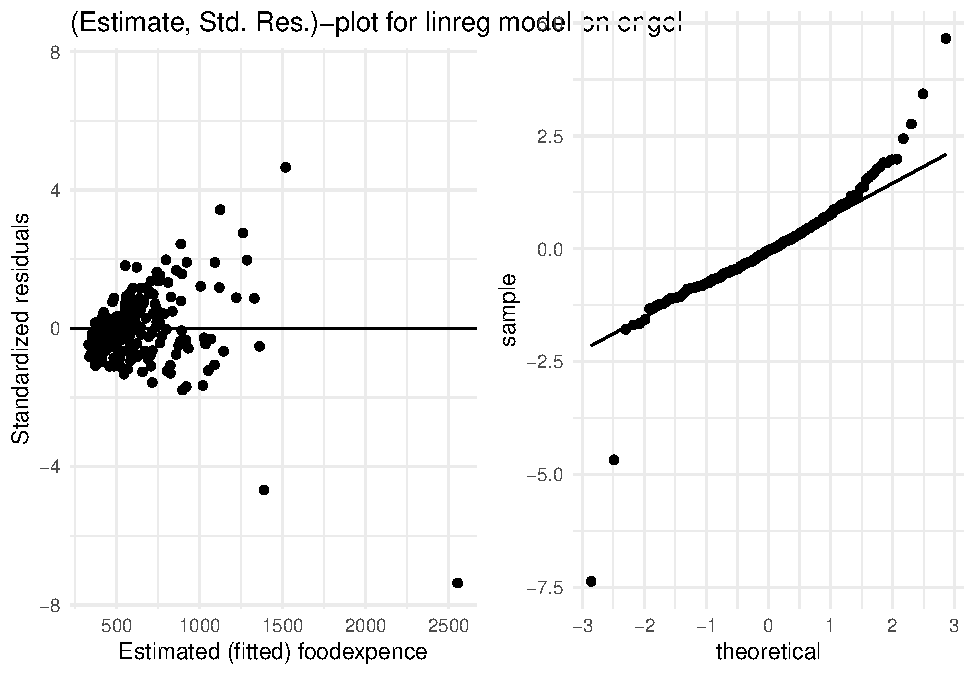
\includegraphics{matstatproblems20-21_files/figure-latex/unnamed-chunk-78-1} \end{center}

From the residual plot we might confirm our suspicions regarding a
non-constant variance, as we see the variance seemingly growing with
increases in mean such that the variance homogeneity assumption seems
unreasonable. There also seems to be a signifigant number of
tail-outliers from the central trend of the qq-plot, we might also
conclude that the normality-assumption regarding \texttt{foodexp} is
also unreasonable.

\hypertarget{section-74}{%
\paragraph{\texorpdfstring{\textbf{3.}}{3.}}\label{section-74}}

With the theory of EH Chapter 11.3 at our back, we may log-transform
both variables;

\begin{Shaded}
\begin{Highlighting}[]
\NormalTok{lfood <-}\StringTok{ }\KeywordTok{log}\NormalTok{(foodexp)}
\NormalTok{lincome <-}\StringTok{ }\KeywordTok{log}\NormalTok{(income)}
\end{Highlighting}
\end{Shaded}

Our new statistical model will be for

\emph{Let \(lfood_1,\ldots lfood_{235}\) independent normally
distributed with variance homogeneity of \(\sigma^2\) and mean
\(Elfood_i=\alpha_l+\beta_l\cdot lincome_i+\epsilon_i,\,\,\epsilon_i\sim\mathcal{N}\left({{0},{\sigma^2}}\right)\,\,i=1,\ldots,235.\)}

One might get the idea that a log-transformation of the ``original
model'', might be prudent, as the log-transform will serve to stabilize
the variability of especially increasing variance values.

We will once again fit a linear regression model noting that the
``linear'' in linear regression relates to how the parameters appear in
the model (thus ``linear'' should really be interpreted as ``affine'').
In 
\includegraphics[width=\textwidth,height=0.16667in]{R_logo.png};

\begin{Shaded}
\begin{Highlighting}[]
\NormalTok{lmodel <-}\StringTok{ }\KeywordTok{lm}\NormalTok{(lincome }\OperatorTok{~}\StringTok{ }\NormalTok{lfood)}
\NormalTok{lfit <-}\StringTok{ }\KeywordTok{fitted}\NormalTok{(lmodel)}
\NormalTok{lrst <-}\StringTok{ }\KeywordTok{rstandard}\NormalTok{(lmodel)}
\NormalTok{p_}\DecValTok{4}\NormalTok{ <-}\StringTok{ }\KeywordTok{qplot}\NormalTok{(lfit, lrst, }\DataTypeTok{main =} \StringTok{"(Estimate, Std. Res.)-plot for log-linreg model on engel"}\NormalTok{, }\DataTypeTok{xlab =} \StringTok{"Estimated (fitted) lfood"}\NormalTok{, }\DataTypeTok{ylab =}\StringTok{"Standardized residuals"}\NormalTok{, }\DataTypeTok{ylim =} \KeywordTok{c}\NormalTok{(}\OperatorTok{-}\KeywordTok{max}\NormalTok{(}\FloatTok{3.2}\NormalTok{,}\KeywordTok{max}\NormalTok{(}\KeywordTok{abs}\NormalTok{(lrst))), }\KeywordTok{max}\NormalTok{(}\FloatTok{3.2}\NormalTok{,}\KeywordTok{max}\NormalTok{(}\KeywordTok{abs}\NormalTok{(lrst)))) )}\OperatorTok{+}\KeywordTok{geom_hline}\NormalTok{(}\DataTypeTok{yintercept =} \DecValTok{0}\NormalTok{) }\CommentTok{#Largest symmetric interval (around 0) of (-3.2,3.2) or (-largest absolute rst, largest absolute rst)}
\NormalTok{p_}\DecValTok{5}\NormalTok{ <-}\StringTok{ }\NormalTok{p }\OperatorTok{+}\StringTok{ }\KeywordTok{geom_qq}\NormalTok{() }\OperatorTok{+}\StringTok{ }\KeywordTok{geom_qq_line}\NormalTok{() }\OperatorTok{+}\StringTok{ }\KeywordTok{aes}\NormalTok{(}\DataTypeTok{sample =}\NormalTok{ lrst)}
\KeywordTok{grid.arrange}\NormalTok{(p_}\DecValTok{4}\NormalTok{,p_}\DecValTok{5}\NormalTok{, }\DataTypeTok{ncol =} \DecValTok{2}\NormalTok{)}
\end{Highlighting}
\end{Shaded}

\begin{center}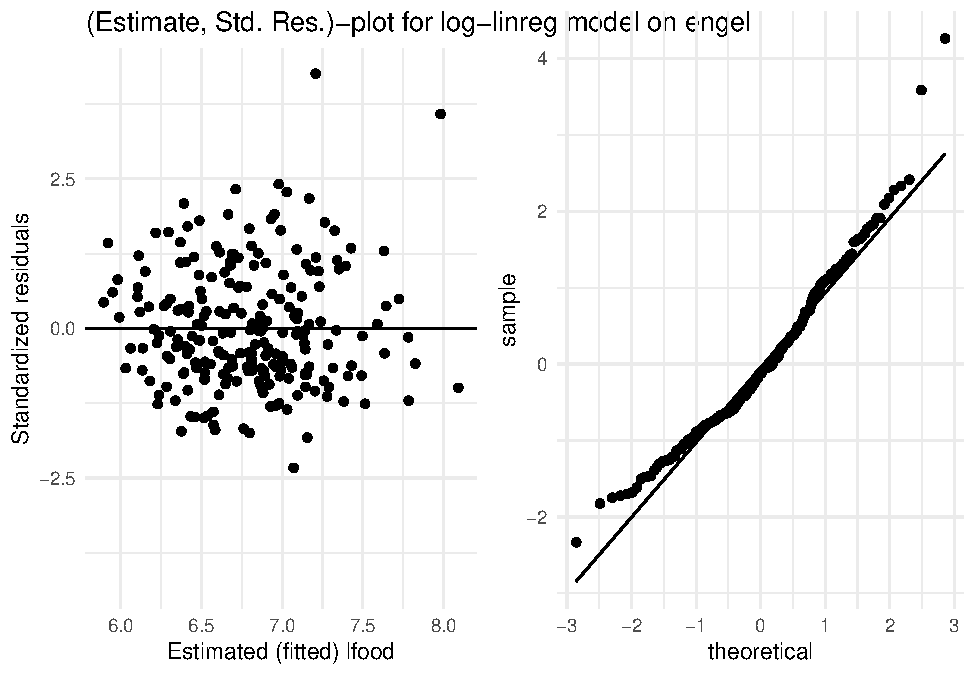
\includegraphics{matstatproblems20-21_files/figure-latex/unnamed-chunk-80-1} \end{center}

The log transformation seem to have done some good, as the residual plot
seem to hold up to both the linearity assumption of the means, and to
the variance homogeneity assumptions, with only a few outliers. The
normality assumption also seems like a rather reasonable approximation,
once again with only a few outliers.

\hypertarget{section-75}{%
\paragraph{\texorpdfstring{\textbf{4.}}{4.}}\label{section-75}}

We may collect the major parameters of the model with

\begin{Shaded}
\begin{Highlighting}[]
\NormalTok{lalpha <-}\StringTok{ }\NormalTok{lmodel}\OperatorTok{$}\NormalTok{coefficients[[}\DecValTok{1}\NormalTok{]]}
\end{Highlighting}
\end{Shaded}

\begin{verbatim}
## [1] 0.2249831
\end{verbatim}

\begin{Shaded}
\begin{Highlighting}[]
\NormalTok{lbeta <-}\StringTok{ }\NormalTok{lmodel}\OperatorTok{$}\NormalTok{coefficients[[}\DecValTok{2}\NormalTok{]]}
\end{Highlighting}
\end{Shaded}

\begin{verbatim}
## [1] 1.032704
\end{verbatim}

\begin{Shaded}
\begin{Highlighting}[]
\NormalTok{ltsigma2 <-}\StringTok{ }\NormalTok{(}\KeywordTok{summary}\NormalTok{(lmodel)}\OperatorTok{$}\NormalTok{sigma)}\OperatorTok{^}\DecValTok{2}
\end{Highlighting}
\end{Shaded}

\begin{verbatim}
## [1] 0.02257692
\end{verbatim}

\hypertarget{section-76}{%
\paragraph{\texorpdfstring{\textbf{5.}}{5.}}\label{section-76}}

For the model in subproblem 3

\hypertarget{section-77}{%
\paragraph{\texorpdfstring{\textbf{6.}}{6.}}\label{section-77}}

\hypertarget{section-78}{%
\paragraph{\texorpdfstring{\textbf{7.}}{7.}}\label{section-78}}

\hypertarget{section-79}{%
\paragraph{\texorpdfstring{\textbf{8.}}{8.}}\label{section-79}}

\hypertarget{section-80}{%
\paragraph{\texorpdfstring{\textbf{9.}}{9.}}\label{section-80}}

\hypertarget{hs-16}{%
\subsection{HS 16}\label{hs-16}}

We may start by importing the dataset

\begin{Shaded}
\begin{Highlighting}[]
\NormalTok{pillbug <-}\StringTok{ }\KeywordTok{read_table2}\NormalTok{(}\StringTok{"M:/Installere/DB/Dropbox/Matematik - Københavns Universitet/3. År/3.3/3.3.A MatStat2020-2021/MatStat Materialer/Interne materialer/Data/pillbug.txt"}\NormalTok{, }
    \DataTypeTok{col_types =} \KeywordTok{cols}\NormalTok{(}\DataTypeTok{group =} \KeywordTok{col_factor}\NormalTok{(}\DataTypeTok{levels =} \KeywordTok{c}\NormalTok{(}\StringTok{"Light"}\NormalTok{, }
        \StringTok{"Moisture"}\NormalTok{, }\StringTok{"Control"}\NormalTok{))))}
\KeywordTok{head}\NormalTok{(pillbug)}
\end{Highlighting}
\end{Shaded}

\begin{verbatim}
## # A tibble: 6 x 2
##    time group
##   <dbl> <fct>
## 1    23 Light
## 2    12 Light
## 3    29 Light
## 4    12 Light
## 5     5 Light
## 6    47 Light
\end{verbatim}

\hypertarget{section-81}{%
\paragraph{\texorpdfstring{\textbf{1.}}{1.}}\label{section-81}}

By EH page 499, the point of a one-sided analysis of variance, is the
test of the model with the assumption that data with the same labels are
to have come from the same normal distribution, while there might be a
difference in mean between the different labels.\textbackslash{} As
such, we may make the experiment in a variety of different ways. The
simplest experiment in which we want to test whether exposure to light
or moisture will affect time, is analysing whether any of the treatments
have an impact at all, through the constant factor system \(L_1.\) In
terms of the one-dimensional analysis of variance, this results from the
\(L_1\) assumption that all the groups will be distributed the same way,
but as one of the treatment is `no treatment', this will be the
hypothesis that there that none of the treatments are effective, ie.
that \(\xi\in L_1,\) such that
\(X_i\sim\mathcal{N}\left({{\xi},{\sigma^2}}\right) \forall i\in I.\)
\textbackslash{} As such we would be looking at the model that in

\includegraphics[width=\textwidth,height=0.16667in]{R_logo.png}
constructed via the following \texttt{lm}-commands, with the thereon
following designmatrix.
\textcolor{red}{{Not sure about the design matrix}}

\begin{Shaded}
\begin{Highlighting}[]
\NormalTok{lm_L1 <-}\StringTok{ }\KeywordTok{lm}\NormalTok{(pillbug}\OperatorTok{$}\NormalTok{time }\OperatorTok{~}\StringTok{ }\DecValTok{1}\NormalTok{, }\DataTypeTok{data =}\NormalTok{ pillbug)}
\KeywordTok{model.matrix}\NormalTok{(pillbug}\OperatorTok{$}\NormalTok{time }\OperatorTok{~}\StringTok{ }\DecValTok{1}\NormalTok{, }\DataTypeTok{data =}\NormalTok{ pillbug)}
\end{Highlighting}
\end{Shaded}

\begin{verbatim}
##    (Intercept)
## 1            1
## 2            1
## 3            1
## 4            1
## 5            1
## 6            1
## 7            1
## 8            1
## 9            1
## 10           1
## 11           1
## 12           1
## 13           1
## 14           1
## 15           1
## 16           1
## 17           1
## 18           1
## 19           1
## 20           1
## 21           1
## 22           1
## 23           1
## 24           1
## 25           1
## 26           1
## 27           1
## 28           1
## 29           1
## 30           1
## 31           1
## 32           1
## 33           1
## 34           1
## 35           1
## 36           1
## 37           1
## 38           1
## 39           1
## 40           1
## 41           1
## 42           1
## 43           1
## 44           1
## 45           1
## 46           1
## 47           1
## 48           1
## 49           1
## 50           1
## 51           1
## 52           1
## 53           1
## 54           1
## 55           1
## 56           1
## 57           1
## 58           1
## 59           1
## 60           1
## attr(,"assign")
## [1] 0
\end{verbatim}

Alternatively, we may look at the one-sided variance through the lens of
the hypotheses that there really might be a difference in effect of the
different treatments. When dealing with the `treatment' factor
\texttt{group} we may therefore construct the analysis in
\includegraphics[width=\textwidth,height=0.16667in]{R_logo.png} as is
done in the following code chunk. Note in particular that the first
uncommented line is present in order to change the intercept reference
from being that of the alphabetically first factor, to \texttt{Control}
- One might compare the derived design matrices with and without this
relevelling. See also \texttt{reorder()} and \texttt{factor()}. Note
also that multiple use of \texttt{relevel} might do the required
permuting of the levels as is seen in the commented line.

\begin{Shaded}
\begin{Highlighting}[]
\CommentTok{#pillbug$group <- relevel(pillbug$group, ref = "Moisture") #relevel M before C, gives order; C, M, L}
\NormalTok{pillbug}\OperatorTok{$}\NormalTok{group <-}\StringTok{ }\KeywordTok{relevel}\NormalTok{(pillbug}\OperatorTok{$}\NormalTok{group, }\DataTypeTok{ref =} \StringTok{"Control"}\NormalTok{)}
\NormalTok{lm_LG <-}\StringTok{ }\KeywordTok{lm}\NormalTok{(time }\OperatorTok{~}\StringTok{ }\NormalTok{group, }\DataTypeTok{data =}\NormalTok{ pillbug)}
\KeywordTok{model.matrix}\NormalTok{(time }\OperatorTok{~}\StringTok{ }\NormalTok{group, }\DataTypeTok{data =}\NormalTok{ pillbug)}
\end{Highlighting}
\end{Shaded}

\begin{verbatim}
##    (Intercept) groupLight groupMoisture
## 1            1          1             0
## 2            1          1             0
## 3            1          1             0
## 4            1          1             0
## 5            1          1             0
## 6            1          1             0
## 7            1          1             0
## 8            1          1             0
## 9            1          1             0
## 10           1          1             0
## 11           1          1             0
## 12           1          1             0
## 13           1          1             0
## 14           1          1             0
## 15           1          1             0
## 16           1          1             0
## 17           1          1             0
## 18           1          1             0
## 19           1          1             0
## 20           1          1             0
## 21           1          0             1
## 22           1          0             1
## 23           1          0             1
## 24           1          0             1
## 25           1          0             1
## 26           1          0             1
## 27           1          0             1
## 28           1          0             1
## 29           1          0             1
## 30           1          0             1
## 31           1          0             1
## 32           1          0             1
## 33           1          0             1
## 34           1          0             1
## 35           1          0             1
## 36           1          0             1
## 37           1          0             1
## 38           1          0             1
## 39           1          0             1
## 40           1          0             1
## 41           1          0             0
## 42           1          0             0
## 43           1          0             0
## 44           1          0             0
## 45           1          0             0
## 46           1          0             0
## 47           1          0             0
## 48           1          0             0
## 49           1          0             0
## 50           1          0             0
## 51           1          0             0
## 52           1          0             0
## 53           1          0             0
## 54           1          0             0
## 55           1          0             0
## 56           1          0             0
## 57           1          0             0
## 58           1          0             0
## 59           1          0             0
## 60           1          0             0
## attr(,"assign")
## [1] 0 1 1
## attr(,"contrasts")
## attr(,"contrasts")$group
## [1] "contr.treatment"
\end{verbatim}

\hypertarget{section-82}{%
\paragraph{\texorpdfstring{\textbf{2.}}{2.}}\label{section-82}}

As requested, we will be trying the command

\begin{Shaded}
\begin{Highlighting}[]
\KeywordTok{boxplot}\NormalTok{(time}\OperatorTok{~}\NormalTok{group, }\DataTypeTok{data=}\NormalTok{pillbug)}
\end{Highlighting}
\end{Shaded}

\includegraphics{matstatproblems20-21_files/figure-latex/unnamed-chunk-85-1.pdf}
Having seen the result, we might investigate its origin, and the
functionality of the \texttt{boxplot} command with \texttt{?boxplot}. As
such, the whiskers mark the minimum and maximum of the data excluding
`outliers'. The main body of the boxplot is the \emph{Inter Quantile
Range (IQR)} of the \(25^{th}, 50^{th}, 75^{th}\) percentile quantile,
noting that the \(50^{th}\) is the median, and is marked by the filled
line, in each of the groups. We might do the similar plot in
\texttt{ggplot2} with

\hypertarget{section-83}{%
\paragraph{\texorpdfstring{\textbf{3.}}{3.}}\label{section-83}}

\hypertarget{section-84}{%
\paragraph{\texorpdfstring{\textbf{4.}}{4.}}\label{section-84}}

\hypertarget{section-85}{%
\paragraph{\texorpdfstring{\textbf{5.}}{5.}}\label{section-85}}

\hypertarget{section-86}{%
\paragraph{\texorpdfstring{\textbf{6.}}{6.}}\label{section-86}}

\hypertarget{hs-17}{%
\subsection{HS 17}\label{hs-17}}

\hypertarget{section-87}{%
\paragraph{\texorpdfstring{\textbf{1.}}{1.}}\label{section-87}}

\hypertarget{section-88}{%
\paragraph{\texorpdfstring{\textbf{2.}}{2.}}\label{section-88}}

\hypertarget{section-89}{%
\paragraph{\texorpdfstring{\textbf{3.}}{3.}}\label{section-89}}

\hypertarget{section-90}{%
\paragraph{\texorpdfstring{\textbf{4.}}{4.}}\label{section-90}}

\hypertarget{section-91}{%
\paragraph{\texorpdfstring{\textbf{5.}}{5.}}\label{section-91}}

\hypertarget{hs-18}{%
\subsection{HS 18}\label{hs-18}}

\hypertarget{section-92}{%
\paragraph{\texorpdfstring{\textbf{1.}}{1.}}\label{section-92}}

\hypertarget{section-93}{%
\paragraph{\texorpdfstring{\textbf{2.}}{2.}}\label{section-93}}

\hypertarget{section-94}{%
\paragraph{\texorpdfstring{\textbf{3.}}{3.}}\label{section-94}}

\begin{center}\rule{0.5\linewidth}{0.5pt}\end{center}

\hypertarget{extra-problems}{%
\section{Extra Problems}\label{extra-problems}}

\hypertarget{extra-5}{%
\subsection{Extra 5}\label{extra-5}}

\hypertarget{extra-6}{%
\subsection{Extra 6}\label{extra-6}}

\hypertarget{extra-8}{%
\subsection{Extra 8}\label{extra-8}}

\hypertarget{extra-on-regression-and-confidence-intervals}{%
\subsection{Extra on Regression and confidence
intervals}\label{extra-on-regression-and-confidence-intervals}}

\textbf{NRH RMD (In Danish)}

Det dokument gennemgår analysen fra EH eksempel 11.13 i R. Dokumentet
viser nogle R-tekniske løsninger, og kommentarerne omkring selve
analysen er meget sparsomme, og skal ikke ses som fyldestgørende for
hvordan en praktisk dataanalyse skal se ud.

Vi vil bruge diverse funktioner fra Tidyverse, så pakken indlæses først.

\begin{Shaded}
\begin{Highlighting}[]
\KeywordTok{library}\NormalTok{(tidyverse)}
\end{Highlighting}
\end{Shaded}

Vi indlæser data fra EH eksempel 11.13.

\begin{Shaded}
\begin{Highlighting}[]
\NormalTok{CAPM <-}\StringTok{ }\KeywordTok{read_csv}\NormalTok{(}\StringTok{"CAPM.csv"}\NormalTok{)}
\end{Highlighting}
\end{Shaded}

\begin{verbatim}
## Parsed with column specification:
## cols(
##   Month = col_character(),
##   r = col_double(),
##   M = col_double(),
##   R = col_double()
## )
\end{verbatim}

Scatter plots af de tre variable mod hinanden.

\begin{Shaded}
\begin{Highlighting}[]
\KeywordTok{qplot}\NormalTok{(r, R, }\DataTypeTok{data =}\NormalTok{ CAPM, }\DataTypeTok{size =} \KeywordTok{I}\NormalTok{(}\DecValTok{3}\NormalTok{), }\DataTypeTok{color =} \KeywordTok{I}\NormalTok{(}\StringTok{"blue"}\NormalTok{))}
\KeywordTok{qplot}\NormalTok{(M, R, }\DataTypeTok{data =}\NormalTok{ CAPM, }\DataTypeTok{size =} \KeywordTok{I}\NormalTok{(}\DecValTok{3}\NormalTok{), }\DataTypeTok{color =} \KeywordTok{I}\NormalTok{(}\StringTok{"blue"}\NormalTok{))}
\KeywordTok{qplot}\NormalTok{(r, M, }\DataTypeTok{data =}\NormalTok{ CAPM, }\DataTypeTok{size =} \KeywordTok{I}\NormalTok{(}\DecValTok{3}\NormalTok{), }\DataTypeTok{color =} \KeywordTok{I}\NormalTok{(}\StringTok{"blue"}\NormalTok{))}
\end{Highlighting}
\end{Shaded}

\includegraphics[width=0.32\linewidth]{matstatproblems20-21_files/figure-latex/unnamed-chunk-88-1}
\includegraphics[width=0.32\linewidth]{matstatproblems20-21_files/figure-latex/unnamed-chunk-88-2}
\includegraphics[width=0.32\linewidth]{matstatproblems20-21_files/figure-latex/unnamed-chunk-88-3}

Vi kan også plotte af de tre variable over tid, som giver god mening for
det her datasæt.

\begin{Shaded}
\begin{Highlighting}[]
\KeywordTok{qplot}\NormalTok{(}\KeywordTok{factor}\NormalTok{(Month, }\DataTypeTok{levels =}\NormalTok{ Month), R, }\DataTypeTok{data =}\NormalTok{ CAPM, }\DataTypeTok{size =} \KeywordTok{I}\NormalTok{(}\DecValTok{2}\NormalTok{), }\DataTypeTok{color =} \KeywordTok{I}\NormalTok{(}\StringTok{"blue"}\NormalTok{)) }\OperatorTok{+}\StringTok{ }\KeywordTok{geom_line}\NormalTok{(}\KeywordTok{aes}\NormalTok{(}\DataTypeTok{group =} \DecValTok{1}\NormalTok{), }\DataTypeTok{color =} \StringTok{"blue"}\NormalTok{)}
\KeywordTok{qplot}\NormalTok{(}\KeywordTok{factor}\NormalTok{(Month, }\DataTypeTok{levels =}\NormalTok{ Month), M, }\DataTypeTok{data =}\NormalTok{ CAPM, }\DataTypeTok{size =} \KeywordTok{I}\NormalTok{(}\DecValTok{2}\NormalTok{), }\DataTypeTok{color =} \KeywordTok{I}\NormalTok{(}\StringTok{"red"}\NormalTok{)) }\OperatorTok{+}\StringTok{ }\KeywordTok{geom_line}\NormalTok{(}\KeywordTok{aes}\NormalTok{(}\DataTypeTok{group =} \DecValTok{1}\NormalTok{), }\DataTypeTok{color =} \StringTok{"red"}\NormalTok{)}
\KeywordTok{qplot}\NormalTok{(}\KeywordTok{factor}\NormalTok{(Month, }\DataTypeTok{levels =}\NormalTok{ Month), r, }\DataTypeTok{data =}\NormalTok{ CAPM, }\DataTypeTok{size =} \KeywordTok{I}\NormalTok{(}\DecValTok{2}\NormalTok{), }\DataTypeTok{color =} \KeywordTok{I}\NormalTok{(}\StringTok{"violet"}\NormalTok{)) }\OperatorTok{+}\StringTok{ }\KeywordTok{geom_line}\NormalTok{(}\KeywordTok{aes}\NormalTok{(}\DataTypeTok{group =} \DecValTok{1}\NormalTok{), }\DataTypeTok{color =} \StringTok{"violet"}\NormalTok{)}
\end{Highlighting}
\end{Shaded}

\includegraphics{matstatproblems20-21_files/figure-latex/unnamed-chunk-89-1.pdf}
\includegraphics{matstatproblems20-21_files/figure-latex/unnamed-chunk-89-2.pdf}
\includegraphics{matstatproblems20-21_files/figure-latex/unnamed-chunk-89-3.pdf}

Vi genfinder nu den fittede model fra EH eksempel 11.13.

\begin{Shaded}
\begin{Highlighting}[]
\NormalTok{CAPM_lm <-}\StringTok{ }\KeywordTok{lm}\NormalTok{(R }\OperatorTok{~}\StringTok{ }\NormalTok{M }\OperatorTok{+}\StringTok{ }\NormalTok{r, }\DataTypeTok{data =}\NormalTok{ CAPM)}
\KeywordTok{summary}\NormalTok{(CAPM_lm)}
\end{Highlighting}
\end{Shaded}

\begin{verbatim}
## 
## Call:
## lm(formula = R ~ M + r, data = CAPM)
## 
## Residuals:
##      Min       1Q   Median       3Q      Max 
## -16.7829  -2.6282  -0.4654   3.4771  11.5701 
## 
## Coefficients:
##             Estimate Std. Error t value Pr(>|t|)  
## (Intercept) -10.0837     6.1645  -1.636   0.1203  
## M             0.1556     0.3371   0.462   0.6502  
## r            29.0208    14.4096   2.014   0.0601 .
## ---
## Signif. codes:  0 '***' 0.001 '**' 0.01 '*' 0.05 '.' 0.1 ' ' 1
## 
## Residual standard error: 6.394 on 17 degrees of freedom
## Multiple R-squared:  0.2035, Adjusted R-squared:  0.1098 
## F-statistic: 2.171 on 2 and 17 DF,  p-value: 0.1446
\end{verbatim}

Vi kan konstruere designmatricen ved ``håndkraft'' fra data på følgende
måde:

\begin{Shaded}
\begin{Highlighting}[]
\NormalTok{A <-}\StringTok{ }\KeywordTok{matrix}\NormalTok{(}\KeywordTok{c}\NormalTok{(}\KeywordTok{rep}\NormalTok{(}\DecValTok{1}\NormalTok{, }\DecValTok{20}\NormalTok{), CAPM}\OperatorTok{$}\NormalTok{M, CAPM}\OperatorTok{$}\NormalTok{r), }\DataTypeTok{nrow =} \DecValTok{20}\NormalTok{)}
\NormalTok{A}
\end{Highlighting}
\end{Shaded}

\begin{verbatim}
##       [,1]   [,2]  [,3]
##  [1,]    1  8.549 0.496
##  [2,]    1 -0.173 0.510
##  [3,]    1  4.199 0.532
##  [4,]    1 -0.630 0.569
##  [5,]    1 -0.565 0.543
##  [6,]    1  5.106 0.581
##  [7,]    1  7.012 0.543
##  [8,]    1 -0.346 0.475
##  [9,]    1  6.312 0.370
## [10,]    1  2.949 0.316
## [11,]    1 -1.556 0.340
## [12,]    1  2.432 0.316
## [13,]    1  8.631 0.309
## [14,]    1  0.123 0.315
## [15,]    1 10.174 0.314
## [16,]    1 -4.737 0.350
## [17,]    1  2.498 0.334
## [18,]    1 -5.460 0.346
## [19,]    1  0.921 0.351
## [20,]    1  5.283 0.371
\end{verbatim}

Vi kan nu genfinde estimaterne ved løsning af et lineært ligningssystem.

\begin{Shaded}
\begin{Highlighting}[]
\KeywordTok{solve}\NormalTok{(}\KeywordTok{t}\NormalTok{(A) }\OperatorTok\StringTok{ }\NormalTok{A, }\KeywordTok{t}\NormalTok{(A) }\OperatorTok\StringTok{ }\NormalTok{CAPM}\OperatorTok{$}\NormalTok{R)}
\end{Highlighting}
\end{Shaded}

\begin{verbatim}
##             [,1]
## [1,] -10.0837178
## [2,]   0.1555781
## [3,]  29.0207852
\end{verbatim}

Designmatricen kan vi også trække ud af lm-objektet eller konstruere
direkte med funktionen \texttt{model.matrix()}

\begin{Shaded}
\begin{Highlighting}[]
\KeywordTok{model.matrix}\NormalTok{(CAPM_lm)}
\end{Highlighting}
\end{Shaded}

\begin{verbatim}
##    (Intercept)      M     r
## 1            1  8.549 0.496
## 2            1 -0.173 0.510
## 3            1  4.199 0.532
## 4            1 -0.630 0.569
## 5            1 -0.565 0.543
## 6            1  5.106 0.581
## 7            1  7.012 0.543
## 8            1 -0.346 0.475
## 9            1  6.312 0.370
## 10           1  2.949 0.316
## 11           1 -1.556 0.340
## 12           1  2.432 0.316
## 13           1  8.631 0.309
## 14           1  0.123 0.315
## 15           1 10.174 0.314
## 16           1 -4.737 0.350
## 17           1  2.498 0.334
## 18           1 -5.460 0.346
## 19           1  0.921 0.351
## 20           1  5.283 0.371
## attr(,"assign")
## [1] 0 1 2
\end{verbatim}

\begin{Shaded}
\begin{Highlighting}[]
\KeywordTok{model.matrix}\NormalTok{(}\OperatorTok{~}\StringTok{ }\NormalTok{M }\OperatorTok{+}\StringTok{ }\NormalTok{r, }\DataTypeTok{data =}\NormalTok{ CAPM)}
\end{Highlighting}
\end{Shaded}

\begin{verbatim}
##    (Intercept)      M     r
## 1            1  8.549 0.496
## 2            1 -0.173 0.510
## 3            1  4.199 0.532
## 4            1 -0.630 0.569
## 5            1 -0.565 0.543
## 6            1  5.106 0.581
## 7            1  7.012 0.543
## 8            1 -0.346 0.475
## 9            1  6.312 0.370
## 10           1  2.949 0.316
## 11           1 -1.556 0.340
## 12           1  2.432 0.316
## 13           1  8.631 0.309
## 14           1  0.123 0.315
## 15           1 10.174 0.314
## 16           1 -4.737 0.350
## 17           1  2.498 0.334
## 18           1 -5.460 0.346
## 19           1  0.921 0.351
## 20           1  5.283 0.371
## attr(,"assign")
## [1] 0 1 2
\end{verbatim}

Først plotter vi de rå residualer

\begin{Shaded}
\begin{Highlighting}[]
\KeywordTok{qplot}\NormalTok{(}\KeywordTok{fitted}\NormalTok{(CAPM_lm), }\KeywordTok{residuals}\NormalTok{(CAPM_lm)) }\OperatorTok{+}\StringTok{ }
\StringTok{    }\KeywordTok{geom_hline}\NormalTok{(}\DataTypeTok{yintercept =} \DecValTok{0}\NormalTok{) }\OperatorTok{+}
\StringTok{    }\KeywordTok{geom_smooth}\NormalTok{()}
\end{Highlighting}
\end{Shaded}

\begin{verbatim}
## `geom_smooth()` using method = 'loess' and formula 'y ~ x'
\end{verbatim}

\includegraphics{matstatproblems20-21_files/figure-latex/unnamed-chunk-94-1.pdf}

og dernæst residualerne standardiseret med det centrale estimat for
spredningen.

\begin{Shaded}
\begin{Highlighting}[]
\NormalTok{sigma_hat <-}\StringTok{ }\KeywordTok{sqrt}\NormalTok{(}\KeywordTok{sum}\NormalTok{(}\KeywordTok{residuals}\NormalTok{(CAPM_lm)}\OperatorTok{^}\DecValTok{2}\NormalTok{) }\OperatorTok{/}\StringTok{ }\DecValTok{17}\NormalTok{)  }\CommentTok{# Centralt variansestimate}
\KeywordTok{qplot}\NormalTok{(}\KeywordTok{fitted}\NormalTok{(CAPM_lm), }\KeywordTok{residuals}\NormalTok{(CAPM_lm) }\OperatorTok{/}\StringTok{ }\NormalTok{sigma_hat) }\OperatorTok{+}\StringTok{ }
\StringTok{    }\KeywordTok{geom_hline}\NormalTok{(}\DataTypeTok{yintercept =} \DecValTok{0}\NormalTok{) }\OperatorTok{+}
\StringTok{    }\KeywordTok{geom_hline}\NormalTok{(}\DataTypeTok{yintercept =} \DecValTok{-2}\NormalTok{, }\DataTypeTok{linetype =} \DecValTok{2}\NormalTok{) }\OperatorTok{+}
\StringTok{    }\KeywordTok{geom_hline}\NormalTok{(}\DataTypeTok{yintercept =} \DecValTok{2}\NormalTok{, }\DataTypeTok{linetype =} \DecValTok{2}\NormalTok{) }\OperatorTok{+}
\StringTok{    }\KeywordTok{geom_smooth}\NormalTok{() }\OperatorTok{+}
\StringTok{    }\KeywordTok{ylim}\NormalTok{(}\OperatorTok{-}\DecValTok{3}\NormalTok{, }\DecValTok{3}\NormalTok{)}
\end{Highlighting}
\end{Shaded}

\begin{verbatim}
## `geom_smooth()` using method = 'loess' and formula 'y ~ x'
\end{verbatim}

\includegraphics{matstatproblems20-21_files/figure-latex/unnamed-chunk-95-1.pdf}

Endelig plotter vi de standardiserede residualer (røde nedenfor), hvor
der altså også er devideret med \(\sqrt{1 - h_{ii}}\), sammenholdt med
residualerne ovenfor.

\begin{Shaded}
\begin{Highlighting}[]
\KeywordTok{qplot}\NormalTok{(}\KeywordTok{fitted}\NormalTok{(CAPM_lm), }\KeywordTok{rstandard}\NormalTok{(CAPM_lm), }\DataTypeTok{color =} \KeywordTok{I}\NormalTok{(}\StringTok{"red"}\NormalTok{)) }\OperatorTok{+}\StringTok{ }
\StringTok{    }\KeywordTok{geom_point}\NormalTok{(}\KeywordTok{aes}\NormalTok{(}\DataTypeTok{y =} \KeywordTok{residuals}\NormalTok{(CAPM_lm) }\OperatorTok{/}\StringTok{ }\NormalTok{sigma_hat)) }\OperatorTok{+}\StringTok{ }
\StringTok{    }\KeywordTok{geom_hline}\NormalTok{(}\DataTypeTok{yintercept =} \DecValTok{0}\NormalTok{) }\OperatorTok{+}
\StringTok{    }\KeywordTok{geom_hline}\NormalTok{(}\DataTypeTok{yintercept =} \DecValTok{-2}\NormalTok{, }\DataTypeTok{linetype =} \DecValTok{2}\NormalTok{) }\OperatorTok{+}
\StringTok{    }\KeywordTok{geom_hline}\NormalTok{(}\DataTypeTok{yintercept =} \DecValTok{2}\NormalTok{, }\DataTypeTok{linetype =} \DecValTok{2}\NormalTok{) }\OperatorTok{+}
\StringTok{    }\KeywordTok{geom_smooth}\NormalTok{() }\OperatorTok{+}
\StringTok{    }\KeywordTok{ylim}\NormalTok{(}\OperatorTok{-}\DecValTok{3}\NormalTok{, }\DecValTok{3}\NormalTok{)}
\end{Highlighting}
\end{Shaded}

\begin{verbatim}
## `geom_smooth()` using method = 'loess' and formula 'y ~ x'
\end{verbatim}

\includegraphics{matstatproblems20-21_files/figure-latex/unnamed-chunk-96-1.pdf}

Man kan observere, at effekten af division med \(\sqrt{1 - h_{ii}}\) er
ganske lille, men alle observationerne flytter udad. Vi kan udtrække
\(h_{ii}\) fra lm-objektet med \texttt{hatvalues()}, hvis vi vil.

\begin{Shaded}
\begin{Highlighting}[]
\KeywordTok{range}\NormalTok{(}\DecValTok{1} \OperatorTok{/}\StringTok{ }\KeywordTok{sqrt}\NormalTok{(}\DecValTok{1} \OperatorTok{-}\StringTok{ }\KeywordTok{hatvalues}\NormalTok{(CAPM_lm)))}
\end{Highlighting}
\end{Shaded}

\begin{verbatim}
## [1] 1.040627 1.170057
\end{verbatim}

For det her eksempel er det også værd at se på residualerne som funktion
af tid, og lave et lag-plot for at se, om der er afhængighed.

\begin{Shaded}
\begin{Highlighting}[]
\KeywordTok{qplot}\NormalTok{(}\DecValTok{1}\OperatorTok{:}\DecValTok{20}\NormalTok{, }\KeywordTok{rstandard}\NormalTok{(CAPM_lm)) }\OperatorTok{+}\StringTok{ }
\StringTok{    }\KeywordTok{geom_smooth}\NormalTok{()}
\end{Highlighting}
\end{Shaded}

\begin{verbatim}
## `geom_smooth()` using method = 'loess' and formula 'y ~ x'
\end{verbatim}

\begin{Shaded}
\begin{Highlighting}[]
\KeywordTok{qplot}\NormalTok{(}\KeywordTok{rstandard}\NormalTok{(CAPM_lm)[}\OperatorTok{-}\DecValTok{20}\NormalTok{], }\KeywordTok{rstandard}\NormalTok{(CAPM_lm)[}\OperatorTok{-}\DecValTok{1}\NormalTok{]) }\OperatorTok{+}\StringTok{ }
\StringTok{    }\KeywordTok{geom_smooth}\NormalTok{(}\DataTypeTok{method =} \StringTok{"lm"}\NormalTok{)}
\end{Highlighting}
\end{Shaded}

\includegraphics[width=0.5\linewidth]{matstatproblems20-21_files/figure-latex/unnamed-chunk-98-1}
\includegraphics[width=0.5\linewidth]{matstatproblems20-21_files/figure-latex/unnamed-chunk-98-2}

Lag-plottet indikerer, at fejlene er negativt korrelerede.

Vi kan også lave et QQ-plot for at undersøge normalfordelingsantagelsen.
Med kun 20 observationer er det ganske svært at afvise
normalfordelingen.

\begin{Shaded}
\begin{Highlighting}[]
\KeywordTok{qqnorm}\NormalTok{(}\KeywordTok{rstandard}\NormalTok{(CAPM_lm))}
\KeywordTok{qqline}\NormalTok{(}\KeywordTok{rstandard}\NormalTok{(CAPM_lm))}
\end{Highlighting}
\end{Shaded}

\includegraphics{matstatproblems20-21_files/figure-latex/unnamed-chunk-99-1.pdf}

Konfidensintervaller

Vi kan til slut genfinde konfidensintervallerne fra EH ved at bruge
\texttt{confint()} på lm-objektet. Den omsætter estimater og standard
errors til standard konfidensintervaller baseret på den korrekte
\(t\)-fordeling.

\begin{Shaded}
\begin{Highlighting}[]
\KeywordTok{confint}\NormalTok{(CAPM_lm)}
\end{Highlighting}
\end{Shaded}

\begin{verbatim}
##                   2.5 %     97.5 %
## (Intercept) -23.0895931  2.9221576
## M            -0.5555732  0.8667294
## r            -1.3808162 59.4223867
\end{verbatim}

Reducerer vi modellen ved at fjerne interceptet fås et noget anderledes
estimat, og en reduktion i standard errors for \(\hat{\gamma}\). Det
skyldes primært at \(r\) varierer ganske lidt og interceptsøjlen og
\(r\) kommer til at være tæt på hinanden. Om de ligefrem er tæt på at
være kollineære er til diskussion.

\begin{Shaded}
\begin{Highlighting}[]
\NormalTok{CAPM_lm_}\DecValTok{0}\NormalTok{ <-}\StringTok{ }\KeywordTok{lm}\NormalTok{(R }\OperatorTok{~}\StringTok{ }\NormalTok{M }\OperatorTok{+}\StringTok{ }\NormalTok{r }\OperatorTok{-}\StringTok{ }\DecValTok{1}\NormalTok{, }\DataTypeTok{data =}\NormalTok{ CAPM)}
\KeywordTok{summary}\NormalTok{(CAPM_lm_}\DecValTok{0}\NormalTok{)}
\end{Highlighting}
\end{Shaded}

\begin{verbatim}
## 
## Call:
## lm(formula = R ~ M + r - 1, data = CAPM)
## 
## Residuals:
##      Min       1Q   Median       3Q      Max 
## -18.1457  -3.1795  -0.7022   3.3169   9.2088 
## 
## Coefficients:
##   Estimate Std. Error t value Pr(>|t|)
## M  0.09853    0.35052   0.281    0.782
## r  6.32644    4.07043   1.554    0.138
## 
## Residual standard error: 6.685 on 18 degrees of freedom
## Multiple R-squared:  0.1799, Adjusted R-squared:  0.08875 
## F-statistic: 1.974 on 2 and 18 DF,  p-value: 0.1678
\end{verbatim}

\begin{Shaded}
\begin{Highlighting}[]
\KeywordTok{confint}\NormalTok{(CAPM_lm_}\DecValTok{0}\NormalTok{)}
\end{Highlighting}
\end{Shaded}

\begin{verbatim}
##        2.5 %     97.5 %
## M -0.6378792  0.8349428
## r -2.2252161 14.8780969
\end{verbatim}

\begin{Shaded}
\begin{Highlighting}[]
\NormalTok{CAPM <-}\StringTok{ }\KeywordTok{read_csv}\NormalTok{(}\StringTok{"CAPM.csv"}\NormalTok{)}
\end{Highlighting}
\end{Shaded}

\begin{verbatim}
## Parsed with column specification:
## cols(
##   Month = col_character(),
##   r = col_double(),
##   M = col_double(),
##   R = col_double()
## )
\end{verbatim}

\hypertarget{section-95}{%
\paragraph{\texorpdfstring{\textbf{1.}}{1.}}\label{section-95}}

Our main focus is the CAPM-inspired regression-model from EH example
11.13 of \[
R_i\equiv \alpha + \beta M_i + \gamma r_i + \epsilon_i,
\] for \(\epsilon_1,\ldots,\epsilon_N\) iid.
\(\sim\mathcal{N}\left({{0},{\sigma^2}}\right)\) for some \(\sigma>0,\)
such that \(R_1,\ldots,R_N\) are assumed independent normally
distributed with variance homogeneity of \(\sigma^2,\) and mean \[
ER_i=\alpha+\beta M_i+\gamma r_i + 0.
\] Define \(\theta\equiv\left({\alpha, \beta, \gamma}\right)^T\) such
that we may find a designmatrix \(A\) such that \[
R_i= A\theta+\epsilon\equiv \begin{pmatrix}{\alpha\\\beta\\\gamma}\end{pmatrix}A+\begin{pmatrix}{\epsilon_1\\\,\vdots\\\epsilon_N}\end{pmatrix}\equiv A_{,1}\alpha + A_{,2}\beta + A_{,3}\gamma + \begin{pmatrix}{\epsilon_1\\\,\vdots\\\epsilon_N}\end{pmatrix}
\] Note as \(\epsilon\in M_{N,1},\theta\in M_{3,1}\) that we thus need
to have \(A\in M_{N,3}.\) Further, we will necessarily need to have \[
a_{1,j}=1,\quad a_{2,j}=M_j,\quad a_{3,j}=r_j,\quad \text{for } j=1,\ldots,N.
\] Consequently, our central assumption of \(R_1,\ldots,R_N\)
independent normally distributed with variance homogeneity may thus for
\(R:=\left({R_1,\ldots,R_N}\right)^T\) be written as \[
R\sim\mathcal{N}\left({{\begin{pmatrix}{ER_1\\ \,\,\vdots\\ ER_N}\end{pmatrix}},{\sigma^2I}}\right)\equiv\mathcal{N}\left({{\begin{pmatrix}{\alpha+\beta M_1+\gamma r_1\\ \quad \quad \quad \vdots\\\alpha+\beta M_N+\gamma r_N}\end{pmatrix}},{\sigma^2I}}\right)\equiv\mathcal{N}\left({{A\theta},{\sigma^2I}}\right).
\] We may define the designmatrix in
\includegraphics[width=\textwidth,height=0.16667in]{R_logo.png}

\begin{Shaded}
\begin{Highlighting}[]
\NormalTok{N <-}\StringTok{ }\KeywordTok{nrow}\NormalTok{(CAPM)}
\NormalTok{k <-}\StringTok{ }\DecValTok{3}
\NormalTok{R <-}\StringTok{ }\NormalTok{CAPM}\OperatorTok{$}\NormalTok{R}
\NormalTok{A <-}\StringTok{ }\KeywordTok{matrix}\NormalTok{(}\KeywordTok{c}\NormalTok{(}\KeywordTok{rep}\NormalTok{(}\DecValTok{1}\NormalTok{,}\DecValTok{20}\NormalTok{),CAPM}\OperatorTok{$}\NormalTok{M,CAPM}\OperatorTok{$}\NormalTok{r), }\DataTypeTok{nrow =}\NormalTok{ N, }\DataTypeTok{ncol =}\NormalTok{ k) }\CommentTok{#bycol=T is default.}
\NormalTok{A}
\end{Highlighting}
\end{Shaded}

\begin{verbatim}
##       [,1]   [,2]  [,3]
##  [1,]    1  8.549 0.496
##  [2,]    1 -0.173 0.510
##  [3,]    1  4.199 0.532
##  [4,]    1 -0.630 0.569
##  [5,]    1 -0.565 0.543
##  [6,]    1  5.106 0.581
##  [7,]    1  7.012 0.543
##  [8,]    1 -0.346 0.475
##  [9,]    1  6.312 0.370
## [10,]    1  2.949 0.316
## [11,]    1 -1.556 0.340
## [12,]    1  2.432 0.316
## [13,]    1  8.631 0.309
## [14,]    1  0.123 0.315
## [15,]    1 10.174 0.314
## [16,]    1 -4.737 0.350
## [17,]    1  2.498 0.334
## [18,]    1 -5.460 0.346
## [19,]    1  0.921 0.351
## [20,]    1  5.283 0.371
\end{verbatim}

\textbf{Alternative definition of \texttt{A} in
\includegraphics[width=\textwidth,height=0.16667in]{R_logo.png}} As
\(A\) is very much defined via its columns, we may use the
\texttt{cbind} function to construct our matrix;

\begin{Shaded}
\begin{Highlighting}[]
\NormalTok{A <-}\StringTok{ }\KeywordTok{cbind}\NormalTok{(}\KeywordTok{rep}\NormalTok{(}\DecValTok{1}\NormalTok{,}\DecValTok{20}\NormalTok{),CAPM}\OperatorTok{$}\NormalTok{M, CAPM}\OperatorTok{$}\NormalTok{r)}
\end{Highlighting}
\end{Shaded}

We may then use the results of K10.21 of EH to conclude that the MLE of
\(\theta\) may be found in
\includegraphics[width=\textwidth,height=0.16667in]{R_logo.png} as

\begin{Shaded}
\begin{Highlighting}[]
\NormalTok{MLETheta <-}\StringTok{ }\KeywordTok{solve}\NormalTok{(}\KeywordTok{t}\NormalTok{(A)}\OperatorTok\NormalTok{A)}\OperatorTok\KeywordTok{t}\NormalTok{(A)}\OperatorTok\NormalTok{CAPM}\OperatorTok{$}\NormalTok{R}
\end{Highlighting}
\end{Shaded}

Also by EH K10.21 the variance matrix of \(\hat\theta\) will be
\(\sim\mathcal{N}\left({{\theta},{\sigma^2\left({A^TA}\right)^{-1}}}\right),\)
which we by EH K10.21 may find in
\includegraphics[width=\textwidth,height=0.16667in]{R_logo.png} through

\begin{Shaded}
\begin{Highlighting}[]
\NormalTok{sigmat2 <-}\StringTok{ }\KeywordTok{as.numeric}\NormalTok{((}\KeywordTok{t}\NormalTok{(R)}\OperatorTok\NormalTok{R}\OperatorTok{-}\KeywordTok{t}\NormalTok{(MLETheta)}\OperatorTok\KeywordTok{t}\NormalTok{(A)}\OperatorTok\NormalTok{A}\OperatorTok\NormalTok{MLETheta)}\OperatorTok{/}\NormalTok{(N}\OperatorTok{-}\NormalTok{k)) }
\end{Highlighting}
\end{Shaded}

\begin{verbatim}
## [1] 40.88448
\end{verbatim}

\begin{Shaded}
\begin{Highlighting}[]
\NormalTok{thetaCovMat <-}\StringTok{ }\NormalTok{sigmat2}\OperatorTok{*}\KeywordTok{solve}\NormalTok{(}\KeywordTok{t}\NormalTok{(A)}\OperatorTok\NormalTok{A)}
\end{Highlighting}
\end{Shaded}

\begin{verbatim}
##             [,1]       [,2]        [,3]
## [1,]  38.0005763 -0.2149795 -85.5238319
## [2,]  -0.2149795  0.1136148  -0.1766915
## [3,] -85.5238319 -0.1766915 207.6366120
\end{verbatim}

Noting that defining \(\tilde\sigma^2=\)\texttt{sigmat2} with
\texttt{as.numeric} is rather important in accordance with not
generating errors in the subsequent multiplication defining
\texttt{thetaCovMat}.

\hypertarget{section-96}{%
\paragraph{\texorpdfstring{\textbf{2.}}{2.}}\label{section-96}}

With the above calculated distribution of
\(\hat\theta\equiv\left({\hat\alpha,\,\hat\beta,\,\hat\gamma}\right)^T\)
we may by EH L9.47 conclude that \[
\hat\beta\sim\mathcal{N}\left({{\beta},{\sigma^2\left({A^TA}\right)^{-1}_{2,2}}}\right)\overset{\cdot}{=}\mathcal{N}\left({{\beta},{0.1136148}}\right),\\
\hat\gamma\sim\mathcal{N}\left({{\gamma},{\sigma^2\left({A^TA}\right)^{-1}_{3,3}}}\right)\overset{\cdot}{=}\mathcal{N}\left({{\gamma},{207.636612}}\right).
\] But more importantly
\(\hat\beta+\hat\gamma=\left({0,1,1}\right)\hat\theta,\) such that we by
K9.46 of EH may conclude that \[
\hat\beta+\hat\gamma=\left({0,1,1}\right)\hat\theta\sim\mathcal{N}\left({{\left({0,1,1}\right)\theta},{\,\left({0,1,1}\right)\sigma^2\left({A^TA}\right)^{-1}\begin{pmatrix}{0\\1\\1}\end{pmatrix}}}\right)\\
=\mathcal{N}\left({{\beta+\gamma},{\,\left({0,1,1}\right)\sigma^2\left({A^TA}\right)^{-1}\begin{pmatrix}{0\\1\\1}\end{pmatrix}}}\right)
\] with the above variance matrix calculated in
\includegraphics[width=\textwidth,height=0.16667in]{R_logo.png} as

\begin{Shaded}
\begin{Highlighting}[]
\NormalTok{selector <-}\StringTok{ }\KeywordTok{matrix}\NormalTok{(}\KeywordTok{c}\NormalTok{(}\DecValTok{0}\NormalTok{,}\DecValTok{1}\NormalTok{,}\DecValTok{1}\NormalTok{),}\DataTypeTok{nrow=}\DecValTok{1}\NormalTok{)}
\NormalTok{bgvar <-}\StringTok{ }\KeywordTok{as.numeric}\NormalTok{(selector}\OperatorTok\NormalTok{thetaCovMat}\OperatorTok\KeywordTok{t}\NormalTok{(selector))}
\end{Highlighting}
\end{Shaded}

\begin{verbatim}
## [1] 207.3968
\end{verbatim}

As such, if we wanted to write the distribution of
\(\hat\beta+\hat\gamma\) on the form
\(\hat\beta+\hat\gamma\sim\mathcal{N}\left({{\beta+\gamma},{se^2}}\right)\)
we should choose \(\tilde{se}^2=\)\texttt{bgvar}\(=207.3968439,\) such
that \(\tilde{se}=14.4012792.\)

Having calculated the central estimator for
\(\sigma,\,\tilde\sigma=40.8844839\) writing
\(se^2=\sigma^2\cdot a\approx\tilde\sigma^2\cdot a,\) we may find \(a\)
as \[
a=\frac{se^2}{\sigma^2}\underset{\sim}{\overset{\cdot}{=}}\frac{207.3968439}{40.8844839}=5.0727519
\]

\hypertarget{section-97}{%
\paragraph{\texorpdfstring{\textbf{3.}}{3.}}\label{section-97}}

\hypertarget{section-98}{%
\paragraph{\texorpdfstring{\textbf{4.}}{4.}}\label{section-98}}

\begin{center}\rule{0.5\linewidth}{0.5pt}\end{center}

\hypertarget{eh-problems}{%
\section{EH problems}\label{eh-problems}}

\hypertarget{eh-9.4}{%
\subsection{EH 9.4}\label{eh-9.4}}

\hypertarget{eh-9.7}{%
\subsection{EH 9.7}\label{eh-9.7}}

\hypertarget{eh-9.12}{%
\subsection{EH 9.12}\label{eh-9.12}}

\hypertarget{eh-9.13}{%
\subsection{EH 9.13}\label{eh-9.13}}

\hypertarget{eh-9.20}{%
\subsection{EH 9.20}\label{eh-9.20}}

\hypertarget{eh-10.5}{%
\subsection{EH 10.5}\label{eh-10.5}}

For \(X_1,X_2,X_3,X_4,X_5\) independent normally distributed, each with
same variance \(\sigma^2>0\), and individual expectation given by \[
EX_1=\alpha_1,\quad EX_2=\alpha_1-\alpha_2,\quad EX_3 = \alpha_1-\alpha_2,\quad EX_4 = \alpha_1+\alpha_2,\quad EX_5 = \alpha_1+\alpha_2,
\] for some \(\alpha_1,\alpha_2\in\mathbb{R}\) being unknown parameters.

\hypertarget{a}{%
\paragraph{\texorpdfstring{\textbf{a)}}{a)}}\label{a}}

Assume we have observed outcomes of the \(X\)'s such that \(X_i=x_i\)
with \(x_i\) as assigned below

\begin{Shaded}
\begin{Highlighting}[]
\NormalTok{X <-}\StringTok{ }\KeywordTok{c}\NormalTok{(}\OperatorTok{-}\FloatTok{0.187}\NormalTok{,}\OperatorTok{-}\FloatTok{1.731}\NormalTok{,}\OperatorTok{-}\FloatTok{0.184}\NormalTok{,}\FloatTok{2.252}\NormalTok{,}\FloatTok{1.775}\NormalTok{)}
\end{Highlighting}
\end{Shaded}

Note that as \(X\equiv\left({X_1,\ldots,X_5}\right)^T\) is a boundling
of five random variables and is perceived as a columnvector as such,
heed that as
\(\alpha\equiv\left({\alpha_1,\alpha_2}\right)^T\in M_{2,1}(\mathbb{R}),\)
we will for \(A\alpha\) being our expected value vector
(\(\in M_{5,1}(\mathbb{R})\)) need \(A\in M_{5,2}(\mathbb{R}).\)

Consequently, observe \[
A\alpha \equiv \begin{pmatrix}
a_{1,1} & a_{1,2}\\
a_{2,1} & a_{2,2}\\
a_{3,1} & a_{3,2}\\
a_{4,1} & a_{4,2}\\
a_{5,1} & a_{5,2}
\end{pmatrix}\begin{pmatrix}{\alpha_1\\\alpha_2}\end{pmatrix}\equiv\begin{pmatrix}{a_{1,1}\\a_{2,1}\\a_{3,1}\\a_{4,1}\\a_{5,1}}\end{pmatrix}\alpha_1+\begin{pmatrix}{a_{1,2}\\a_{2,2}\\a_{3,2}\\a_{4,2}\\a_{5,2}}\end{pmatrix}\alpha_2,
\] such that as we are seeking
\(\begin{pmatrix}{\alpha_1\\\alpha_1-\alpha_2\\\alpha_1-\alpha_2\\\alpha_1+\alpha_2\\\alpha_1+\alpha_2}\end{pmatrix}\equiv EX=A\alpha,\)
we may read off the ``coefficients'' columns of \(\alpha_1\) and
\(\alpha_2\) with \(a_{i,1}=1,\,i=1,\ldots,5,\) and
\(a_{1,2}=0,\,a_{2,2}=-1,\,a_{3,2}=-1,\,a_{4,2}=1,\,a_{5,2}=1,\) such
that \[
A:=\begin{pmatrix}
1&0\\
1&-1\\
1&-1\\
1&1\\
1&1,
\end{pmatrix}
\] will be our designated designmatrix.

In accordance with K10.21 in EH we may define our designmatrix in
\includegraphics[width=\textwidth,height=0.16667in]{R_logo.png} as

\begin{Shaded}
\begin{Highlighting}[]
\NormalTok{A <-}\StringTok{ }\KeywordTok{matrix}\NormalTok{(}\KeywordTok{c}\NormalTok{(}\DecValTok{1}\NormalTok{,}\DecValTok{0}\NormalTok{,}\DecValTok{1}\NormalTok{,}\OperatorTok{-}\DecValTok{1}\NormalTok{,}\DecValTok{1}\NormalTok{,}\OperatorTok{-}\DecValTok{1}\NormalTok{,}\DecValTok{1}\NormalTok{,}\DecValTok{1}\NormalTok{,}\DecValTok{1}\NormalTok{,}\DecValTok{1}\NormalTok{), }\DataTypeTok{nrow =} \DecValTok{5}\NormalTok{, }\DataTypeTok{ncol =} \DecValTok{2}\NormalTok{, }\DataTypeTok{byrow =}\NormalTok{ T) }\CommentTok{#By col is default}
\end{Highlighting}
\end{Shaded}

By EH K10.21 we will have \(\hat\alpha = \left({A^TA}\right)^{-1}A^TX\)
and as such we may define in
\includegraphics[width=\textwidth,height=0.16667in]{R_logo.png}

\begin{Shaded}
\begin{Highlighting}[]
\NormalTok{puA <-}\StringTok{ }\KeywordTok{solve}\NormalTok{(}\KeywordTok{t}\NormalTok{(A)}\OperatorTok\NormalTok{A)}\OperatorTok\KeywordTok{t}\NormalTok{(A)}
\NormalTok{alphahat <-}\StringTok{ }\NormalTok{puA}\OperatorTok\NormalTok{X}
\end{Highlighting}
\end{Shaded}

\begin{verbatim}
##        [,1]
## [1,] 0.3850
## [2,] 1.4855
\end{verbatim}

and as such we may therefore conclude that the MLE for \(\alpha\),
\(\hat\alpha\equiv\begin{pmatrix}{\hat\alpha_1\\\hat\alpha_2}\end{pmatrix}=\begin{pmatrix}{0.385\\1.4855}\end{pmatrix}.\)

\hypertarget{b}{%
\paragraph{\texorpdfstring{\textbf{b)}}{b)}}\label{b}}

By page 413 in EH for \(A\) being a
\(N\times k\overset{\cdot}{=}5\times 2\) matrix we will by page 415 have
that we may estimate \(\tilde\sigma^2\) on the basis of data as \[
\tilde{\sigma}^2=\frac{X^TX-\hat{\alpha}^TA^TA\hat{\alpha}}{N-k}\overset{\cdot}{=}\frac{X^TX-\hat{\alpha}^TA^TA\hat{\alpha}}{3}
\] which we may calculate in
\includegraphics[width=\textwidth,height=0.16667in]{R_logo.png} with

\begin{Shaded}
\begin{Highlighting}[]
\NormalTok{sigmatilde2 <-}\StringTok{ }\KeywordTok{as.numeric}\NormalTok{((}\KeywordTok{t}\NormalTok{(X)}\OperatorTok\NormalTok{X}\OperatorTok{-}\KeywordTok{t}\NormalTok{(alphahat)}\OperatorTok\KeywordTok{t}\NormalTok{(A)}\OperatorTok\NormalTok{A}\OperatorTok\NormalTok{alphahat)}\OperatorTok{/}\DecValTok{3}\NormalTok{) }\CommentTok{#does as.numeric change further calculations?}
\end{Highlighting}
\end{Shaded}

\begin{verbatim}
## [1] 0.5731163
\end{verbatim}

\hypertarget{c}{%
\paragraph{\texorpdfstring{\textbf{c)}}{c)}}\label{c}}

By EH K10.21 we have that the MLE for expected value, \(\hat\alpha\) and
MLE for variance, \(\hat\sigma^2\) are independent, and as such, as the
centralized estimator for the variance
\(\tilde{\sigma}^2:=N\frac{\hat\sigma^2}{N-k},\) we get by measurable
transformations that we will also have independence of MLE for expected
value, \(\hat\alpha,\) and \(\tilde\sigma^2.\)

By independence we get that the joint density of \(\hat\alpha\) and
\(\tilde\sigma^2\) can be obtained throught the product of the marginal
densities. Note in this regard that by K10.21

\[
\hat\alpha\sim\mathcal{N}(\alpha,\sigma^2\left({A^TA}\right)^{-1})
\] and \[
\hat\sigma^2\sim\frac{\sigma^2}{N}\chi^2_{N-k}
\] as in \(\hat\sigma^2\) is \(\chi^2\) distributed with \(k\) degrees
of freedom and ``scale-parameter'' \(\frac{\sigma^2}{N}\) which in
itself is to be interpreted in the sense that the
\(\frac{1}{\frac{\sigma^2}{N}}\hat\sigma^2\equiv\frac{N}{\sigma^2}\hat\sigma^2\sim\chi^2_{N-k}\)
is ``proper'' \(\chi^2\) distributed with \(N-k\) degrees of freedom.
Consequently as \(\tilde{\sigma}^2:=N\frac{\hat\sigma^2}{N-k},\) we will
therefore have that \[
\tilde\sigma^2\sim N\frac{\frac{\sigma^2}{N}}{N-k}\chi^2_{N-k}\equiv\frac{\sigma^2}{N-k}\chi^2_{N-k}.
\] The density for some \(Q\sim\chi_q^2\) is
\(\frac{1}{2^{\frac{q}{2}}\Gamma(\frac{q}{2})}x^{\frac{q}{2}-1}e^{-\frac{x}{2}}\)
such that we will have that the density of \(\tilde\sigma^2\) is going
to be \begin{align*}
f_{\tilde\sigma^2}(x)\equiv f_{\frac{\sigma^2}{N-k}\chi_{N-k}^2}(x)&=\frac{N-k}{\sigma^2}\frac{1}{2^{\frac{N-k}{2}}\Gamma(\frac{N-k}{2})}x^{\frac{N-k}{2}-1}e^{-\frac{x}{2}}\overset{\cdot}{=}\frac{5-2}{\sigma^2}\frac{1}{2^{\frac{5-2}{2}}\Gamma(\frac{5-2}{2})}x^{\frac{5-2}{2}-1}e^{-\frac{x}{2}}\\
&\equiv \frac{3}{\sigma^2}\frac{1}{2^{\frac{3}{2}}\Gamma(\frac{3}{2})}x^{\frac{3}{2}-1}e^{-\frac{x}{2}},
\end{align*} hence, as for \(f_{\hat\alpha}\) being the density for
\(\hat\alpha\) we get that the joint density of \(\hat\alpha\) and
\(\tilde\sigma^2,\) \(f_{\hat\alpha,\tilde\sigma^2}\) will be \[
f_{\hat\alpha,\tilde\sigma^2}=f_{\hat\alpha}(x)\cdot f_{\tilde\sigma^2}(x).
\]

\hypertarget{d}{%
\paragraph{\texorpdfstring{\textbf{d)}}{d)}}\label{d}}

We may deploy one of two methods, in order to calculate confidence
intervals for \(\alpha_1,\alpha_2.\)

\textbf{Method 1: EH Example 10.30}

Note that we by a) may write \[
X\equiv\left({X_1,\ldots,X_5}\right)^T\sim\mathcal{N}\left({{A\alpha},{\sigma^2I}}\right).
\] Define
\(\varphi_1:\mathbb{R}^2\rightarrow\mathbb{R},\,\varphi_2:\mathbb{R}^2\rightarrow\mathbb{R},\)
for
\(\omega\equiv\begin{pmatrix}{\omega_1\\\omega_2}\end{pmatrix}\in\mathbb{R}^2\)
as the coordinate projections
\(\varphi_1(\omega):=\omega_1,\,\varphi_2(\omega):=\omega_2\)
respectively. For
\(e_1:=\begin{pmatrix}{1\\0}\end{pmatrix},\,e_2:=\begin{pmatrix}{0\\1}\end{pmatrix},\)
observe \[
\varphi_1(\omega)=e_1^T\omega=\omega_1,\quad\varphi_2(\omega)=e_2^T\omega=\omega_2.
\] \(1-\alpha^*\) confidence intervals for
\(\varphi_1(\alpha)=\alpha_1,\,\varphi_2(\alpha)=\alpha_2\) may be
obtained as \begin{align}
KI_{\alpha_1}&=\left({e_1^T\hat\alpha-\sqrt{e_1^T\left({A^TA}\right)^{-1}e_1f_{\alpha^*}\tilde\sigma^2},\,e_1^T\hat\alpha+\sqrt{e_1^T\left({A^TA}\right)^{-1}e_1f_{\alpha^*}\tilde\sigma^2}}\right)\\
KI_{\alpha_2}&=\left({e_2^T\hat\alpha-\sqrt{e_2^T\left({A^TA}\right)^{-1}e_2f_{\alpha^*}\tilde\sigma^2},\,e_2^T\hat\alpha+\sqrt{e_2^T\left({A^TA}\right)^{-1}e_2f_{\alpha^*}\tilde\sigma^2}}\right)
\end{align} by EH Example 10.30, with \(f_{\alpha^*}\) being the
\(1-\alpha^*\) quantile for the \(F\)-distribution with
\(\left({1,N-k}\right)\) degrees of freedom, for
\(A\in M_{N,k}\overset{\cdot}{=}M_{5,2}\) of rank
\(k\overset{\cdot}{=}2\).

Having looked through \texttt{?qf}, an implementation in
\includegraphics[width=\textwidth,height=0.16667in]{R_logo.png} for
\(\alpha^*=0.05\) may be obtained with

\begin{Shaded}
\begin{Highlighting}[]
\NormalTok{falphastar <-}\StringTok{ }\KeywordTok{qf}\NormalTok{(}\DataTypeTok{p =} \FloatTok{0.95}\NormalTok{, }\DataTypeTok{df1 =} \DecValTok{1}\NormalTok{, }\DataTypeTok{df2 =} \KeywordTok{nrow}\NormalTok{(A)}\OperatorTok{-}\KeywordTok{ncol}\NormalTok{(A)) }\CommentTok{#f_\{\textbackslash{}alpha^*\}}
\NormalTok{e_}\DecValTok{1}\NormalTok{ <-}\StringTok{ }\KeywordTok{c}\NormalTok{(}\DecValTok{1}\NormalTok{,}\DecValTok{0}\NormalTok{)}
\NormalTok{e_}\DecValTok{2}\NormalTok{ <-}\StringTok{ }\KeywordTok{c}\NormalTok{(}\DecValTok{0}\NormalTok{,}\DecValTok{1}\NormalTok{)}
\NormalTok{sqhelper_}\DecValTok{1}\NormalTok{ <-}\StringTok{ }\KeywordTok{as.numeric}\NormalTok{(}\KeywordTok{sqrt}\NormalTok{(}\KeywordTok{t}\NormalTok{(e_}\DecValTok{1}\NormalTok{)}\OperatorTok\KeywordTok{solve}\NormalTok{(}\KeywordTok{t}\NormalTok{(A)}\OperatorTok\NormalTok{A)}\OperatorTok\NormalTok{e_}\DecValTok{1}\OperatorTok{*}\NormalTok{falphastar}\OperatorTok{*}\NormalTok{sigmatilde2))}
\end{Highlighting}
\end{Shaded}

\begin{verbatim}
## [1] 1.077451
\end{verbatim}

\begin{Shaded}
\begin{Highlighting}[]
\NormalTok{sqhelper_}\DecValTok{2}\NormalTok{ <-}\StringTok{ }\KeywordTok{as.numeric}\NormalTok{(}\KeywordTok{sqrt}\NormalTok{(}\KeywordTok{t}\NormalTok{(e_}\DecValTok{2}\NormalTok{)}\OperatorTok\KeywordTok{solve}\NormalTok{(}\KeywordTok{t}\NormalTok{(A)}\OperatorTok\NormalTok{A)}\OperatorTok\NormalTok{e_}\DecValTok{2}\OperatorTok{*}\NormalTok{falphastar}\OperatorTok{*}\NormalTok{sigmatilde2))}
\end{Highlighting}
\end{Shaded}

\begin{verbatim}
## [1] 1.204627
\end{verbatim}

\begin{Shaded}
\begin{Highlighting}[]
\NormalTok{KI_alpha1_}\DecValTok{1}\NormalTok{ <-}\StringTok{ }\KeywordTok{c}\NormalTok{(e_}\DecValTok{1}\OperatorTok\NormalTok{alphahat}\OperatorTok{-}\NormalTok{sqhelper_}\DecValTok{1}\NormalTok{, e_}\DecValTok{1}\OperatorTok\NormalTok{alphahat}\OperatorTok{+}\NormalTok{sqhelper_}\DecValTok{1}\NormalTok{)}
\end{Highlighting}
\end{Shaded}

\begin{verbatim}
## [1] -0.6924509  1.4624509
\end{verbatim}

\begin{Shaded}
\begin{Highlighting}[]
\NormalTok{KI_alpha2_}\DecValTok{1}\NormalTok{ <-}\StringTok{ }\KeywordTok{c}\NormalTok{(e_}\DecValTok{2}\OperatorTok\NormalTok{alphahat}\OperatorTok{-}\NormalTok{sqhelper_}\DecValTok{2}\NormalTok{, e_}\DecValTok{2}\OperatorTok\NormalTok{alphahat}\OperatorTok{+}\NormalTok{sqhelper_}\DecValTok{2}\NormalTok{)}
\end{Highlighting}
\end{Shaded}

\begin{verbatim}
## [1] 0.2808733 2.6901267
\end{verbatim}

Other methods to define the \texttt{sqhelper}'s

Note that we could've also defined the \texttt{sqhelper}'s with

\begin{Shaded}
\begin{Highlighting}[]
\KeywordTok{sqrt}\NormalTok{(}\KeywordTok{solve}\NormalTok{(}\KeywordTok{t}\NormalTok{(A)}\OperatorTok\NormalTok{A)[}\DecValTok{1}\NormalTok{,}\DecValTok{1}\NormalTok{]}\OperatorTok{*}\NormalTok{falphastar}\OperatorTok{*}\NormalTok{sigmatilde2)}
\end{Highlighting}
\end{Shaded}

\begin{verbatim}
## [1] 1.077451
\end{verbatim}

\begin{Shaded}
\begin{Highlighting}[]
\KeywordTok{sqrt}\NormalTok{(}\KeywordTok{solve}\NormalTok{(}\KeywordTok{t}\NormalTok{(A)}\OperatorTok\NormalTok{A)[}\DecValTok{2}\NormalTok{,}\DecValTok{2}\NormalTok{]}\OperatorTok{*}\NormalTok{falphastar}\OperatorTok{*}\NormalTok{sigmatilde2)}
\end{Highlighting}
\end{Shaded}

\begin{verbatim}
## [1] 1.204627
\end{verbatim}

as \(e_i^TBe_i=b_{ii}\) for any standard basisvector \(e_i\) of
appropriate size to be multiplied with some matrix \(B.\) Finally we
might also choose to forego the selection of diagonal element untill it
is needed;

\begin{Shaded}
\begin{Highlighting}[]
\NormalTok{sqhelper <-}\StringTok{ }\KeywordTok{sqrt}\NormalTok{(}\KeywordTok{solve}\NormalTok{(}\KeywordTok{t}\NormalTok{(A)}\OperatorTok\NormalTok{A)}\OperatorTok{*}\NormalTok{falphastar}\OperatorTok{*}\NormalTok{sigmatilde2)}
\NormalTok{sqhelper[}\DecValTok{1}\NormalTok{,}\DecValTok{1}\NormalTok{]}
\end{Highlighting}
\end{Shaded}

\begin{verbatim}
## [1] 1.077451
\end{verbatim}

\begin{Shaded}
\begin{Highlighting}[]
\NormalTok{sqhelper[}\DecValTok{2}\NormalTok{,}\DecValTok{2}\NormalTok{]}
\end{Highlighting}
\end{Shaded}

\begin{verbatim}
## [1] 1.204627
\end{verbatim}

\textbf{Method 2: EH K10.21}

As \[
\hat\alpha\sim\mathcal{N}(\alpha,\sigma^2\left({A^TA}\right)^{-1})\overset{\cdot}{=}\mathcal{N}\left({{\begin{pmatrix}{\alpha_1\\\alpha_2}\end{pmatrix}},{\begin{pmatrix}
\frac{\sigma^2}{5}&0\\
0&\frac{\sigma^2}{4}\end{pmatrix}}}\right)
\] we get by EH L9.47 that \[
\hat\alpha_1\sim\mathcal{N}\left({{\alpha_1},{\frac{\sigma^2}{5}}}\right),\quad\hat\alpha_2\sim\mathcal{N}\left({{\alpha_2},{\frac{\sigma^2}{4}}}\right).
\] By the likes of ``Introduktion til Statistik'' T4.7 we may note that
\[
\hat\alpha_1\pm t_{n-1,1-\frac{\alpha^*}{2}}SE(\hat\alpha_1),\quad\hat\alpha_2\pm t_{n-1,1-\frac{\alpha^*}{2}}SE(\hat\alpha_2),
\] will be \(1-\alpha^*\) confidence intervals for \(\alpha_1,\alpha_2\)
respectively. In our case, we have \(n=5\) datapoints, and are seeking
\(95\%\)-confidence intervals such that \(\alpha^*=0.05.\)

\begin{Shaded}
\begin{Highlighting}[]
\NormalTok{talphastar <-}\StringTok{ }\KeywordTok{qt}\NormalTok{(}\FloatTok{0.975}\NormalTok{,}\DecValTok{4}\NormalTok{) }\CommentTok{#2.776445}
\NormalTok{KI_alpha1_}\DecValTok{2}\NormalTok{ <-}\StringTok{ }\KeywordTok{c}\NormalTok{(alphahat[}\DecValTok{1}\NormalTok{]}\OperatorTok{-}\NormalTok{talphastar}\OperatorTok{*}\KeywordTok{sqrt}\NormalTok{(sigmatilde2}\OperatorTok{*}\KeywordTok{solve}\NormalTok{(}\KeywordTok{t}\NormalTok{(A)}\OperatorTok\NormalTok{A)[}\DecValTok{1}\NormalTok{,}\DecValTok{1}\NormalTok{]), alphahat[}\DecValTok{1}\NormalTok{]}\OperatorTok{+}\NormalTok{talphastar}\OperatorTok{*}\KeywordTok{sqrt}\NormalTok{(sigmatilde2}\OperatorTok{*}\KeywordTok{solve}\NormalTok{(}\KeywordTok{t}\NormalTok{(A)}\OperatorTok\NormalTok{A)[}\DecValTok{1}\NormalTok{,}\DecValTok{1}\NormalTok{]))}
\end{Highlighting}
\end{Shaded}

\begin{verbatim}
## [1] -0.5549949  1.3249949
\end{verbatim}

\begin{Shaded}
\begin{Highlighting}[]
\NormalTok{KI_alpha2_}\DecValTok{2}\NormalTok{ <-}\StringTok{ }\KeywordTok{c}\NormalTok{(alphahat[}\DecValTok{2}\NormalTok{]}\OperatorTok{-}\NormalTok{talphastar}\OperatorTok{*}\KeywordTok{sqrt}\NormalTok{(sigmatilde2}\OperatorTok{*}\KeywordTok{solve}\NormalTok{(}\KeywordTok{t}\NormalTok{(A)}\OperatorTok\NormalTok{A)[}\DecValTok{2}\NormalTok{,}\DecValTok{2}\NormalTok{]), alphahat[}\DecValTok{2}\NormalTok{]}\OperatorTok{+}\NormalTok{talphastar}\OperatorTok{*}\KeywordTok{sqrt}\NormalTok{(sigmatilde2}\OperatorTok{*}\KeywordTok{solve}\NormalTok{(}\KeywordTok{t}\NormalTok{(A)}\OperatorTok\NormalTok{A)[}\DecValTok{2}\NormalTok{,}\DecValTok{2}\NormalTok{]))}
\end{Highlighting}
\end{Shaded}

\begin{verbatim}
## [1] 0.4345538 2.5364462
\end{verbatim}

\hypertarget{eh-11.3}{%
\subsection{EH 11.3}\label{eh-11.3}}

We can import the data with

\begin{Shaded}
\begin{Highlighting}[]
\NormalTok{EHopg11dot3 <-}\StringTok{ }\KeywordTok{read_table2}\NormalTok{(}\StringTok{"EHopg11dot3.txt"}\NormalTok{, }
    \DataTypeTok{col_types =} \KeywordTok{cols}\NormalTok{(}\DataTypeTok{Alder =} \KeywordTok{col_integer}\NormalTok{()))}
\end{Highlighting}
\end{Shaded}

\begin{verbatim}
## Warning: 19 parsing failures.
## row col  expected    actual              file
##   2  -- 3 columns 4 columns 'EHopg11dot3.txt'
##   3  -- 3 columns 4 columns 'EHopg11dot3.txt'
##   4  -- 3 columns 4 columns 'EHopg11dot3.txt'
##   5  -- 3 columns 4 columns 'EHopg11dot3.txt'
##   6  -- 3 columns 4 columns 'EHopg11dot3.txt'
## ... ... ......... ......... .................
## See problems(...) for more details.
\end{verbatim}

\hypertarget{a-1}{%
\paragraph{\texorpdfstring{\textbf{a)}}{a)}}\label{a-1}}

We may subset the data according to profession with

\begin{Shaded}
\begin{Highlighting}[]
\NormalTok{jour <-}\StringTok{ }\KeywordTok{subset}\NormalTok{(EHopg11dot3, EHopg11dot3}\OperatorTok{$}\NormalTok{Fag }\OperatorTok{==}\StringTok{ "J"}\NormalTok{)}
\NormalTok{uni <-}\StringTok{  }\KeywordTok{subset}\NormalTok{(EHopg11dot3, EHopg11dot3}\OperatorTok{$}\NormalTok{Fag }\OperatorTok{==}\StringTok{ "U"}\NormalTok{)}
\end{Highlighting}
\end{Shaded}

We may then plot bloodpressure across from age in each of the two
groups;

\begin{Shaded}
\begin{Highlighting}[]
\KeywordTok{plot}\NormalTok{(jour}\OperatorTok{$}\NormalTok{Alder, jour}\OperatorTok{$}\NormalTok{Blodtryk, }\DataTypeTok{ylab =} \StringTok{"Bloodpressure of journalists (mm Hg)"}\NormalTok{, }\DataTypeTok{xlab =} \StringTok{"Years of age"}\NormalTok{)}
\KeywordTok{plot}\NormalTok{(uni}\OperatorTok{$}\NormalTok{Alder, uni}\OperatorTok{$}\NormalTok{Blodtryk, }\DataTypeTok{ylab =} \StringTok{"Bloodpressure of University teachers (mm Hg)"}\NormalTok{, }\DataTypeTok{xlab =} \StringTok{"Years of age"}\NormalTok{)}
\end{Highlighting}
\end{Shaded}

\includegraphics[width=0.5\linewidth]{matstatproblems20-21_files/figure-latex/unnamed-chunk-118-1}
\includegraphics[width=0.5\linewidth]{matstatproblems20-21_files/figure-latex/unnamed-chunk-118-2}
Looking at the plots, we figure that as a function of the low number of
data points, it doesn't look unreasonable to assume that there might be
a linear relation between bloodpressure and age.

\hypertarget{b-1}{%
\paragraph{\texorpdfstring{\textbf{b)}}{b)}}\label{b-1}}

We may steal the statistical model as described in IS D6.1, recited as

\emph{We assume
\(Y_1,\ldots,Y_n \overset{\text{iid.}}{\sim}\mathcal{N}(\alpha+\beta x_i,\sigma^2),\,\)with
\(\alpha,\beta\in\mathbb{R},\,\sigma^2>0\) being unknown parameters.}

for each of the two groupings. Implementing this in
\includegraphics[width=\textwidth,height=0.16667in]{R_logo.png} and
pearing at the summary is done through

\begin{Shaded}
\begin{Highlighting}[]
\NormalTok{jourmodel <-}\StringTok{ }\KeywordTok{lm}\NormalTok{(jour}\OperatorTok{$}\NormalTok{Blodtryk }\OperatorTok{~}\StringTok{ }\NormalTok{jour}\OperatorTok{$}\NormalTok{Alder)}
\KeywordTok{summary}\NormalTok{(jourmodel)}
\end{Highlighting}
\end{Shaded}

\begin{verbatim}
## 
## Call:
## lm(formula = jour$Blodtryk ~ jour$Alder)
## 
## Residuals:
##    Min     1Q Median     3Q    Max 
## -8.644 -2.881  1.274  1.849  7.219 
## 
## Coefficients:
##             Estimate Std. Error t value Pr(>|t|)    
## (Intercept)  84.9952     7.5966   11.19 2.38e-07 ***
## jour$Alder    1.5296     0.1325   11.54 1.74e-07 ***
## ---
## Signif. codes:  0 '***' 0.001 '**' 0.01 '*' 0.05 '.' 0.1 ' ' 1
## 
## Residual standard error: 4.26 on 11 degrees of freedom
## Multiple R-squared:  0.9237, Adjusted R-squared:  0.9168 
## F-statistic: 133.2 on 1 and 11 DF,  p-value: 1.737e-07
\end{verbatim}

just as well as we might draw estimates for \(\alpha_{j},\,\beta_j\) out
of \includegraphics[width=\textwidth,height=0.16667in]{R_logo.png} with

\begin{Shaded}
\begin{Highlighting}[]
\NormalTok{alphaj <-}\StringTok{ }\NormalTok{jourmodel}\OperatorTok{$}\NormalTok{coefficients[[}\DecValTok{1}\NormalTok{]]}
\end{Highlighting}
\end{Shaded}

\begin{verbatim}
## [1] 84.99522
\end{verbatim}

\begin{Shaded}
\begin{Highlighting}[]
\NormalTok{betaj <-}\StringTok{ }\NormalTok{jourmodel}\OperatorTok{$}\NormalTok{coefficients[[}\DecValTok{2}\NormalTok{]]}
\end{Highlighting}
\end{Shaded}

\begin{verbatim}
## [1] 1.529568
\end{verbatim}

\hypertarget{c-1}{%
\paragraph{\texorpdfstring{\textbf{c)}}{c)}}\label{c-1}}

We copy the procedure of subproblem b;

\begin{Shaded}
\begin{Highlighting}[]
\NormalTok{unimodel <-}\StringTok{ }\KeywordTok{lm}\NormalTok{(uni}\OperatorTok{$}\NormalTok{Blodtryk }\OperatorTok{~}\StringTok{ }\NormalTok{uni}\OperatorTok{$}\NormalTok{Alder)}
\KeywordTok{summary}\NormalTok{(unimodel)}
\end{Highlighting}
\end{Shaded}

\begin{verbatim}
## 
## Call:
## lm(formula = uni$Blodtryk ~ uni$Alder)
## 
## Residuals:
##    Min     1Q Median     3Q    Max 
## -8.248 -1.673  1.127  1.602  6.814 
## 
## Coefficients:
##             Estimate Std. Error t value Pr(>|t|)    
## (Intercept)  75.6299    10.2884   7.351 5.58e-06 ***
## uni$Alder     1.5624     0.1817   8.597 1.01e-06 ***
## ---
## Signif. codes:  0 '***' 0.001 '**' 0.01 '*' 0.05 '.' 0.1 ' ' 1
## 
## Residual standard error: 4.41 on 13 degrees of freedom
## Multiple R-squared:  0.8504, Adjusted R-squared:  0.8389 
## F-statistic: 73.91 on 1 and 13 DF,  p-value: 1.008e-06
\end{verbatim}

just as well as we might draw estimates for \(\alpha_{j},\,\beta_j\) out
of \includegraphics[width=\textwidth,height=0.16667in]{R_logo.png} with

\begin{Shaded}
\begin{Highlighting}[]
\NormalTok{alphau <-}\StringTok{ }\NormalTok{unimodel}\OperatorTok{$}\NormalTok{coefficients[[}\DecValTok{1}\NormalTok{]]}
\end{Highlighting}
\end{Shaded}

\begin{verbatim}
## [1] 75.62986
\end{verbatim}

\begin{Shaded}
\begin{Highlighting}[]
\NormalTok{betau <-}\StringTok{ }\NormalTok{unimodel}\OperatorTok{$}\NormalTok{coefficients[[}\DecValTok{2}\NormalTok{]]}
\end{Highlighting}
\end{Shaded}

\begin{verbatim}
## [1] 1.562384
\end{verbatim}

\hypertarget{d-1}{%
\paragraph{\texorpdfstring{\textbf{d)}}{d)}}\label{d-1}}

We may implement an aggregate linear regression model for bloodpressure
across the two groupings, with each group responsible for a set of
parameters. Note however that the standard
\texttt{model\ \textless{}-\ lm(EHopg11dot3\$Blodtryk\ \textasciitilde{}\ jour\$Alder+uni\$Alder)}
won't work, as we are asking to model the \(28\) datapoints of the
dataset based on \(13\) and \(15\) datapoints respectively. Instead note
that what we desire is of the format \[
EX_i=1_J(i)\left({\alpha_J+\beta_Jt_i}\right)+1_U(i)\left({\alpha_U+\beta_Ut_i}\right)
\] As such we may then implement the indicator functions \(1_U,1_J\) in
the estimates ``via the data'', which we will do by creating the matrix

\begin{Shaded}
\begin{Highlighting}[]
\NormalTok{A <-}\KeywordTok{matrix}\NormalTok{(}\KeywordTok{c}\NormalTok{(}\KeywordTok{rep}\NormalTok{(}\DecValTok{1}\NormalTok{,}\DecValTok{13}\NormalTok{),}\KeywordTok{rep}\NormalTok{(}\DecValTok{0}\NormalTok{,}\DecValTok{15}\NormalTok{), jour}\OperatorTok{$}\NormalTok{Alder,}\KeywordTok{rep}\NormalTok{(}\DecValTok{0}\NormalTok{,}\DecValTok{15}\NormalTok{),}\KeywordTok{rep}\NormalTok{(}\DecValTok{0}\NormalTok{,}\DecValTok{13}\NormalTok{),}\KeywordTok{rep}\NormalTok{(}\DecValTok{1}\NormalTok{,}\DecValTok{15}\NormalTok{),}\KeywordTok{rep}\NormalTok{(}\DecValTok{0}\NormalTok{,}\DecValTok{13}\NormalTok{),uni}\OperatorTok{$}\NormalTok{Alder),}\DataTypeTok{nrow=}\DecValTok{28}\NormalTok{)}
\NormalTok{A}
\end{Highlighting}
\end{Shaded}

\begin{verbatim}
##       [,1] [,2] [,3] [,4]
##  [1,]    1   68    0    0
##  [2,]    1   62    0    0
##  [3,]    1   49    0    0
##  [4,]    1   62    0    0
##  [5,]    1   34    0    0
##  [6,]    1   66    0    0
##  [7,]    1   45    0    0
##  [8,]    1   60    0    0
##  [9,]    1   57    0    0
## [10,]    1   57    0    0
## [11,]    1   63    0    0
## [12,]    1   56    0    0
## [13,]    1   57    0    0
## [14,]    0    0    1   55
## [15,]    0    0    1   49
## [16,]    0    0    1   60
## [17,]    0    0    1   54
## [18,]    0    0    1   58
## [19,]    0    0    1   51
## [20,]    0    0    1   43
## [21,]    0    0    1   52
## [22,]    0    0    1   53
## [23,]    0    0    1   61
## [24,]    0    0    1   61
## [25,]    0    0    1   57
## [26,]    0    0    1   57
## [27,]    0    0    1   70
## [28,]    0    0    1   63
\end{verbatim}

We will thus be able to do;

\begin{Shaded}
\begin{Highlighting}[]
\NormalTok{modelgroups <-}\StringTok{ }\KeywordTok{lm}\NormalTok{(EHopg11dot3}\OperatorTok{$}\NormalTok{Blodtryk }\OperatorTok{~}\StringTok{ }\NormalTok{A}\DecValTok{-1}\NormalTok{)}
\KeywordTok{summary}\NormalTok{(modelgroups)}
\end{Highlighting}
\end{Shaded}

\begin{verbatim}
## 
## Call:
## lm(formula = EHopg11dot3$Blodtryk ~ A - 1)
## 
## Residuals:
##    Min     1Q Median     3Q    Max 
## -8.644 -3.019  1.201  1.785  7.219 
## 
## Coefficients:
##    Estimate Std. Error t value Pr(>|t|)    
## A1  84.9952     7.7426  10.978 7.71e-11 ***
## A2   1.5296     0.1351  11.322 4.12e-11 ***
## A3  75.6299    10.1296   7.466 1.05e-07 ***
## A4   1.5624     0.1789   8.732 6.47e-09 ***
## ---
## Signif. codes:  0 '***' 0.001 '**' 0.01 '*' 0.05 '.' 0.1 ' ' 1
## 
## Residual standard error: 4.342 on 24 degrees of freedom
## Multiple R-squared:  0.9994, Adjusted R-squared:  0.9993 
## F-statistic: 1.045e+04 on 4 and 24 DF,  p-value: < 2.2e-16
\end{verbatim}

We may recognize the already calculated estimates in the summary.

\textbf{Pulling estimates from model} The estimates might be found from
\texttt{model} in
\includegraphics[width=\textwidth,height=0.16667in]{R_logo.png} via

\begin{Shaded}
\begin{Highlighting}[]
\NormalTok{modelgroups}\OperatorTok{$}\NormalTok{coefficients[[}\DecValTok{1}\NormalTok{]]}
\NormalTok{modelgroups}\OperatorTok{$}\NormalTok{coefficients[[}\DecValTok{2}\NormalTok{]]}
\NormalTok{modelgroups}\OperatorTok{$}\NormalTok{coefficients[[}\DecValTok{3}\NormalTok{]]}
\NormalTok{modelgroups}\OperatorTok{$}\NormalTok{coefficients[[}\DecValTok{4}\NormalTok{]]}
\end{Highlighting}
\end{Shaded}

\hypertarget{e}{%
\paragraph{\texorpdfstring{\textbf{e)}}{e)}}\label{e}}

We may then finally do a full linear regression model based on the
entire dataset, with no splitting into groups;

\begin{Shaded}
\begin{Highlighting}[]
\NormalTok{model <-}\StringTok{ }\KeywordTok{lm}\NormalTok{(EHopg11dot3}\OperatorTok{$}\NormalTok{Blodtryk}\OperatorTok{~}\NormalTok{EHopg11dot3}\OperatorTok{$}\NormalTok{Alder)}
\end{Highlighting}
\end{Shaded}

The estimates may once again be collected via

\begin{Shaded}
\begin{Highlighting}[]
\NormalTok{alpha <-}\StringTok{ }\NormalTok{model}\OperatorTok{$}\NormalTok{coefficients[[}\DecValTok{1}\NormalTok{]]}
\NormalTok{alpha}
\end{Highlighting}
\end{Shaded}

\begin{verbatim}
## [1] 79.6603
\end{verbatim}

\begin{Shaded}
\begin{Highlighting}[]
\NormalTok{beta <-}\StringTok{ }\NormalTok{model}\OperatorTok{$}\NormalTok{coefficients[[}\DecValTok{2}\NormalTok{]]}
\NormalTok{beta}
\end{Highlighting}
\end{Shaded}

\begin{verbatim}
## [1] 1.552729
\end{verbatim}

\hypertarget{f}{%
\paragraph{\texorpdfstring{\textbf{f)}}{f)}}\label{f}}

\begin{center}\rule{0.5\linewidth}{0.5pt}\end{center}

\hypertarget{nrh-problems}{%
\section{NRH Problems}\label{nrh-problems}}

\hypertarget{nrh-1.1}{%
\subsection{NRH 1.1}\label{nrh-1.1}}

\hypertarget{nrh-1.2}{%
\subsection{NRH 1.2}\label{nrh-1.2}}

\hypertarget{nrh-1.3}{%
\subsection{NRH 1.3}\label{nrh-1.3}}

\hypertarget{nrh-1.4}{%
\subsection{NRH 1.4}\label{nrh-1.4}}

\begin{center}\rule{0.5\linewidth}{0.5pt}\end{center}

\hypertarget{bms-problems}{%
\section{BMS Problems}\label{bms-problems}}

\hypertarget{bms-1.1}{%
\subsection{BMS 1.1}\label{bms-1.1}}

\hypertarget{bms-1.2}{%
\subsection{BMS 1.2}\label{bms-1.2}}

\hypertarget{bms-1.3}{%
\subsection{BMS 1.3}\label{bms-1.3}}

\hypertarget{bms-1.4}{%
\subsection{BMS 1.4}\label{bms-1.4}}

\hypertarget{bms-1.5}{%
\subsection{BMS 1.5}\label{bms-1.5}}

\hypertarget{bms-1.6}{%
\subsection{BMS 1.6}\label{bms-1.6}}

\hypertarget{bms-1.7}{%
\subsection{BMS 1.7}\label{bms-1.7}}

\hypertarget{bms-1.8}{%
\subsection{BMS 1.8}\label{bms-1.8}}

\hypertarget{bms-3.4}{%
\subsection{BMS 3.4}\label{bms-3.4}}

\hypertarget{f-1}{%
\paragraph{\texorpdfstring{\textbf{f)}}{f)}}\label{f-1}}

We may start off by defining various starting parameters;

\begin{Shaded}
\begin{Highlighting}[]
\NormalTok{n <-}\StringTok{ }\DecValTok{10}\OperatorTok{^}\DecValTok{3} \CommentTok{#outcomes}
\NormalTok{mu <-}\StringTok{ }\DecValTok{4}
\NormalTok{delta <-}\StringTok{ }\DecValTok{3}
\NormalTok{reprep <-}\StringTok{ }\DecValTok{10}\OperatorTok{^}\DecValTok{4} \CommentTok{#number of repeated experiments}
\NormalTok{dat <-}\StringTok{ }\KeywordTok{matrix}\NormalTok{(}\OtherTok{NA}\NormalTok{,n,reprep)}
\end{Highlighting}
\end{Shaded}

Then running the simulation of
\texttt{reprep=\textbackslash{}ensuremath\{10\^{}\{4\}\}} datasets of
\texttt{n\ =\ 1000} \(U(\mu-\delta,\mu+\delta)\) datapoints.

\begin{Shaded}
\begin{Highlighting}[]
\ControlFlowTok{for}\NormalTok{ (i }\ControlFlowTok{in} \DecValTok{1}\OperatorTok{:}\NormalTok{reprep) \{}
\NormalTok{  dat[,i] <-}\StringTok{ }\KeywordTok{runif}\NormalTok{(n, }\DataTypeTok{min=}\NormalTok{mu}\OperatorTok{-}\NormalTok{delta, }\DataTypeTok{max =}\NormalTok{ mu}\OperatorTok{+}\NormalTok{delta) }
\NormalTok{\}}

\NormalTok{datMax <-}\StringTok{ }\KeywordTok{apply}\NormalTok{(dat, }\DecValTok{2}\NormalTok{, max) }\CommentTok{#apply the max function to all columns (2) of dat}
\NormalTok{datMin <-}\StringTok{ }\KeywordTok{apply}\NormalTok{(dat, }\DecValTok{2}\NormalTok{, min)}

\CommentTok{#Definitions in problem b)}
\NormalTok{muhat <-}\StringTok{ }\NormalTok{(datMin}\OperatorTok{+}\NormalTok{datMax)}\OperatorTok{/}\DecValTok{2} 
\NormalTok{deltahat <-}\StringTok{ }\NormalTok{(datMax}\OperatorTok{-}\NormalTok{datMin)}\OperatorTok{/}\DecValTok{2}
\end{Highlighting}
\end{Shaded}

Note also that

\begin{Shaded}
\begin{Highlighting}[]
\KeywordTok{mean}\NormalTok{(muhat)}
\end{Highlighting}
\end{Shaded}

\begin{verbatim}
## [1] 3.999997
\end{verbatim}

\begin{Shaded}
\begin{Highlighting}[]
\KeywordTok{mean}\NormalTok{(deltahat)}
\end{Highlighting}
\end{Shaded}

\begin{verbatim}
## [1] 2.993998
\end{verbatim}

We may do histograms of the data

\begin{Shaded}
\begin{Highlighting}[]
\NormalTok{p_}\DecValTok{1}\NormalTok{ <-}\StringTok{ }\KeywordTok{qplot}\NormalTok{(muhat, }\DataTypeTok{geom =} \StringTok{"histogram"}\NormalTok{)}
\NormalTok{p_}\DecValTok{2}\NormalTok{ <-}\StringTok{ }\KeywordTok{qplot}\NormalTok{(deltahat, }\DataTypeTok{geom =} \StringTok{"histogram"}\NormalTok{)}

\KeywordTok{grid.arrange}\NormalTok{(p_}\DecValTok{1}\NormalTok{,p_}\DecValTok{2}\NormalTok{, }\DataTypeTok{ncol =} \DecValTok{2}\NormalTok{)}
\end{Highlighting}
\end{Shaded}

\begin{verbatim}
## `stat_bin()` using `bins = 30`. Pick better value with `binwidth`.
## `stat_bin()` using `bins = 30`. Pick better value with `binwidth`.
\end{verbatim}

\includegraphics{matstatproblems20-21_files/figure-latex/unnamed-chunk-131-1.pdf}

To verify c);

\begin{Shaded}
\begin{Highlighting}[]
\NormalTok{mucheck <-}\StringTok{ }\KeywordTok{apply}\NormalTok{(dat, }\DecValTok{2}\NormalTok{, median)}
\KeywordTok{mean}\NormalTok{(mucheck)}
\end{Highlighting}
\end{Shaded}

\begin{verbatim}
## [1] 4.000673
\end{verbatim}

\begin{Shaded}
\begin{Highlighting}[]
\KeywordTok{qplot}\NormalTok{(mucheck)}
\end{Highlighting}
\end{Shaded}

\begin{verbatim}
## `stat_bin()` using `bins = 30`. Pick better value with `binwidth`.
\end{verbatim}

\includegraphics{matstatproblems20-21_files/figure-latex/unnamed-chunk-132-1.pdf}

\end{document}
